\documentclass[12pt]{report}


% Define margins
\setlength{\topmargin}{-1.0cm}
\setlength{\oddsidemargin}{0.1cm}
\setlength{\textwidth}{16.5cm}
\setlength{\textheight}{23.0cm}







% Define header and footer
\usepackage{lastpage}
\usepackage{fancyhdr}
\pagestyle{fancy}
\fancyhf{}
\lhead{{
\includegraphics[height=.8cm]{figures/nus.png}}}
\rhead{\textbf{\textit{Interpretable and Fair Machine Learning}} }
\lfoot{\textbf{\textit{Page \thepage/\pageref*{LastPage}}}}
\renewcommand{\footrulewidth}{0.7pt}
\renewcommand{\headrulewidth}{0.7pt}



% Packages
\usepackage{amsmath}
\usepackage{amsthm,dsfont,amssymb}
\newtheorem{comment}{Comment}
%\theoremstyle{definition}
\usepackage[utf8]{inputenc} 
\usepackage{graphicx}
\usepackage{multirow}
\usepackage{color}
\usepackage{comment}
\usepackage{microtype}
\usepackage{wrapfig}
\usepackage{hyperref,url}
\usepackage[
font=footnotesize % or small or scriptsize
]{subfig}
\usepackage{booktabs}
\usepackage{caption}
\usepackage{enumitem,kantlipsum}
\usepackage{algorithm}
\usepackage[noend]{algpseudocode}


% Theorem
\newtheorem{theorem}{Theorem}
\newtheorem{definition}{Definition}
\newtheorem{axiom}{Axiom}
\newtheorem{property}[theorem]{Property}
\newtheorem*{remark}{Remark}
\newtheorem{lemma}[theorem]{Lemma}
\newtheorem{lemmarep}{Lemma}
\newtheorem{proposition}[theorem]{Proposition}
\newtheorem{example}{Example}[section]
\newtheorem{corollary}{Corollary}



% Tikz
\usepackage{tikz}
\usetikzlibrary{automata}
\usetikzlibrary{bayesnet,arrows}
\usetikzlibrary{shapes,fit,calc,positioning}
\tikzset{box/.style={draw, diamond, thick, text centered, minimum height=0.5cm, minimum width=1cm, text width=0.9cm}}
\tikzset{line/.style={draw, thick, -latex'}}


% References
\usepackage{cite}
\usepackage[nameinlink,capitalize]{cleveref}  % easy referencing




% Macros
\newcommand{\red}[1]{\textcolor{red}{#1}}
\newcommand{\blue}[1]{\textcolor{blue}{#1}}
\newcommand{\green}[1]{\textcolor{green}{#1}}

% Fairness 
%	Justicia
			\newcommand{\justicia}{\ensuremath{\mathsf{Justicia}}}
			\newcommand{\nonsensitive}{\ensuremath{\mathbf{X}}}
			\newcommand{\sensitive}{\ensuremath{\mathbf{A}}}
			\newcommand{\bool}{\ensuremath{B}}
			\newcommand{\alg}{\mathcal{M}}
			\newcommand{\R}{\ensuremath{\raisebox{\depth}{\rotatebox{180}{R}}}}
			\newcommand{\justiciaenum}{\ensuremath{\mathsf{Justicia\_enum}}}
			\newcommand{\justicialearn}{\ensuremath{\mathsf{Justicia\_learn}}}
			\newcommand{\justiciacond}{\ensuremath{\mathsf{Justicia\_cond}}}
	
%	FVGM
			\newcommand{\fvgm}{\ensuremath{\mathsf{FVGM}}}
			\newcommand{\mediator}{\ensuremath{\mathbf{Z}}}
			\newcommand{\stochastic}{\ensuremath{\mathsf{S3P}}}
			\DeclareMathOperator*{\argmax}{arg\,max}
			\DeclareMathOperator*{\argmin}{arg\,min}
			\newcommand{\graph}{\ensuremath{G}}
			\newcommand{\factors}{\ensuremath{\theta}}
			\newcommand{\parent}{\ensuremath{\mathrm{Pa}}}
			\newcommand{\BN}{\ensuremath{\mathsf{BN}}}
			
%			color
			\definecolor{terminate}{gray}{0.8}
			\definecolor{collision}{rgb}{0.2,1,0.3}
			\definecolor{existential}{rgb}{0.9,0.9, 0.1}
			
			
			
			
			
			


\begin{document}
	\begin{center}
		\Large \textbf{Interpretable and Fair Machine Learning} \\
		\vspace{1em}
		\large Bishwamittra Ghosh
	\end{center}
	
	\chapter{Introduction}
The last decades have witnessed significant progress in machine learning with a host of applications of algorithmic decision-making in different safety-critical domains, such as medical~\cite{erickson2017machine,kaissis2020secure,kononenko2001machine}, law~\cite{kumar2018law,surden2014machine}, education~\cite{luckin2018machine}, and transportation~\cite{peled2019model,zantalis2019review}. In high-stake domains,  machine learning predictions have far-reaching consequences on the end-users~\cite{eshete2021making}. With the aim of applying machine learning for societal goods, there have been increasing efforts to regulate machine learning by imposing interpretability~\cite{rudin2019stop}, fairness~\cite{barocas2017fairness}, robustness~\cite{rauber2017foolbox}, and privacy~\cite{papernot2016towards} in predictions. In this thesis, we focus on the interpretability and fairness aspects of machine learning. The thesis establishes a close integration of formal methods and automated reasoning with machine learning and proposes efficient algorithmic solutions for problems arising in interpretability and fairness in machine learning.

Towards responsible and trustworthy machine learning, we propose two research themes in this thesis: interpretability and fairness of machine learning classifiers. \emph{In interpretable machine learning}, rule-based classifiers effectively represent the decision boundary using a set of rules comprising input features. Interpretable rule-based classifiers not only interpret the decision function but also are applied to explain the prediction of black-box classifiers~\cite{gill2020responsible,lundberg2017unified,moradi2021post,ribeiro2016should,slack2020fooling}, a fundamental research question in explainable artificial intelligence (XAI). In this thesis, we propose efficient algorithms based on incremental learning for interpretable rule-based classifiers. In another research theme of \emph{fairness in machine learning}, unregulated classifiers tend to exhibit bias/unfairness to certain demographic groups in the data unless classifiers are trained with a fairness objective. Consequently, research on fairness centers on quantifying bias using multiple fairness definitions and mitigating bias based on multiple fairness algorithms. In this thesis, we study probabilistic fairness verification problem, where we formally verify the bias of a classifier given the probability distribution of input features. Finally, we explain the sources of bias by formalizing and computing fairness influence functions, a way to quantify the influence of individual and the intersection of multiple features on the bias of a classifier. To summarize our thesis on interpretability and fairness in machine learning, we prioritize on improving the \emph{scalability} and the \emph{accuracy} of solutions\textemdash either or both of which are absent in prior works. 




\section{Interpretable Machine Learning}
The problem in interpretable machine learning is to learn a classifier making interpretable predictions to the end-users. To achieve the interpretability of predictions, decision functions in the form of classification rules such as decision trees,  decision lists, decision sets, etc.\ are particularly effective~\cite{bessiere2009minimising,dash2021lprules,ignatiev2021reasoning,izza2020explaining,lakkaraju2017interpretable,lakkaraju2016interpretable,letham2015interpretable,narodytska2018learning,rivest1987learning,wang2015falling,yu2020optimal}.  At this point, it is important to acknowledge that interpretability is an informal notion, and formalizing it in full generality is challenging. In our context of rule-based classifiers, we use \emph{sparsity of rules} (that is, fewer rules each having fewer Boolean literals), which has been considered a proxy of interpretability in various domains, specifically in the medical domain~\cite{gage2001validation,lakkaraju2019faithful,letham2015interpretable,malioutov2013exact,myers1962myers}.





In the thesis, we study two interpretable rule-based classifiers, characterized by their expressiveness. At first, we study classifiers represented as formulas in propositional logic. In propositional logic, Conjunctive Formal Form (CNF) and Disjunctive Normal Form (DNF) are useful representations of Boolean formulas. Popular interpretable rule-based classifiers such as decision tree, decision lists, and decision sets share the logical structure of CNF/DNF in their representation of the decision function. Thereby, we propose to learn an interpretable CNF classifier, wherein its interpretability is defined by the number of Boolean literals that the formula contains. Compared to CNF, Boolean cardinality constraints are more expressive as they allow numerical bounds on Boolean literals~\cite{sinz2005towards}. Relying on the concept of cardinality constraints to increase expressiveness, our second interpretable rule-based classifier is a logical relaxation of CNF/DNF classifiers, namely \emph{relaxed-}CNF. 


The problem of learning rule-based classifiers is known to be computationally intractable. The earliest tractable approaches for classifiers such as decision trees and decision lists relied on heuristically chosen objective functions and greedy algorithmic techniques~\cite{ClarkN1989,CohenS1999,quinlan2014}. In these approaches, the size of rules is controlled by early stopping,  ad-hoc rule pruning, etc. In recent approaches, the interpretable classification problem is reduced to an optimization problem, where the accuracy and sparsity of rules are optimized jointly~\cite{lakkaraju2016interpretable,narodytska2018learning}. Different optimization solvers such as linear programming~\cite{malioutov2013exact}, sub-modular optimizations~\cite{lakkaraju2016interpretable}, Bayesian optimizations~\cite{letham2015interpretable}, and MaxSAT~\cite{malioutov2018mlic} are then deployed to find the best classifier with maximum accuracy and minimum rule-size. The discrete combinatorial nature of learning rule-based classifiers leads to the intractability of the problem and suffers from scalability issues in large datasets. Therefore, we propose an incremental learning approach by wrapping traditional optimization solvers such as MaxSAT and MILP to efficiently learn rule-based classifiers in a mini-batch learning setting.  Here we summarize the contributions of the thesis on interpretable rule-based machine learning.

\subsection*{Scalability via Incremental Learning}
We propose an incremental learning framework, called $ \imli $~\cite{GMM2022,GM2019},  based on MaxSAT for learning interpretable classification rules expressed in CNF. $ \mathsf{IMLI} $ considers a joint objective function to optimize the accuracy and sparsity of classification rules and learns a rule-based classifier by solving an appropriately designed MaxSAT query. Despite the progress of MaxSAT solving in the last decade, the straightforward MaxSAT-based solution cannot scale to real-world classification datasets of thousands to millions of samples. Therefore, we incorporate an efficient incremental learning technique inside the MaxSAT formulation by integrating mini-batch learning and iterative rule-learning. The resulting framework learns a classifier by iteratively covering the training data, wherein in each iteration, it solves a sequence of smaller MaxSAT queries corresponding to each mini-batch. In our experiments, $ \mathsf{IMLI} $ achieves the best balance among prediction accuracy, interpretability, and scalability. For instance, $ \mathsf{IMLI} $ attains a competitive prediction accuracy and interpretability with respect to existing interpretable classifiers and demonstrates impressive scalability on large datasets where both interpretable and non-interpretable classifiers fail. As an application, we deploy $ \mathsf{IMLI} $ in learning other interpretable representations: DNF classifiers, decision lists, and decision sets.
	
\subsection*{Expressiveness via Logical Relaxation}
We extend our incremental learning framework to learn a more relaxed representation of classification rules with higher expressiveness. Elaborately, we consider relaxed definitions of standard OR/AND operators in propositional logic by allowing exceptions in the construction of a clause and also in the selection of clauses in a rule. Building on these relaxed definitions, we introduce relaxed-CNF classification rules motivated by the popular usage of checklists in the medical domain and the higher expressiveness of Boolean cardinality constraints. Relaxed-CNF generalizes widely employed rule representations including CNF, DNF, and decision sets. While the combinatorial structure of relaxed-CNF rules offers exponential succinctness, the na\"ive learning techniques are computationally expensive. To this end, we propose an incremental mini-batch learning procedure, called $ \mathsf{CRR} $, that employs advances in MILP solvers to efficiently learn relaxed-CNF rules. Our experimental analysis demonstrates that $ \mathsf{CRR} $ can generate relaxed-CNF rules, which are more accurate and sparser compared to the alternative rule-based models.







\section{Fairness in Machine Learning}
As a technology machine learning is oblivious to societal good or bad. The success of machine learning as an accurate predictor, however, finds applications in high-stake decision-making, such as college admission~\cite{martinez2021using}, recidivism prediction~\cite{tollenaar2013method}, job applications~\cite{ajunwa2016hiring} etc. In such applications, the deployed  classifier often demonstrates bias towards certain \emph{sensitive demographic groups} involved in the data~\cite{dwork2012fairness}. For example, a classifier deciding the eligibility of college admission may offer more admission to White-male candidates than to Black-female candidates\textemdash possibly because of the historical bias in the admission data, or the accuracy-centric learning objective of the classifier, or a combination of both~\cite{berk2019accuracy,landy1978correlates,zliobaite2015relation}. Following such phenomena, multiple fairness metrics, such as \textit{statistical parity}, \textit{equalized odds}, \textit{predictive parity} etc, have been proposed to quantify the bias of the classifier. For example, if the classifier in college admission demonstrates a {statistical parity} of $ 0.6 $, it means that White-male candidates are offered admission $ 60\% $ more frequently than Black-female candidates~\cite{besse2021survey,feldman2015certifying,garg2020fairness}. To this end, different fairness enhancing algorithms have been devised to improve fairness with respect to one or multiple fairness metrics. These algorithms try to rectify and mitigate bias in three ways: \textit{pre-processing} the data~\cite{kamiran2012data,zemel2013learning,calmon2017optimized}, \textit{in-processing} the classifier~\cite{zhang2018mitigating}, and \textit{post-processing} the outcomes of a classifier~\cite{kamiran2012decision,hardt2016equality}. Researchers also study fairness attack algorithms to worsen the fairness of a classifier, such as by adding poisoned data samples~\cite{solans2020poisoning}. In the presence of multiple fairness metrics and algorithms, in this thesis, we contribute to two fundamental problems in fairness: (i) probabilistic verification of fairness and (ii) interpreting or explaining of sources of unfairness.


\subsection*{Probabilistic Fairness Verification} The problem in probabilistic fairness verification is to verify the bias of a classifier given the distribution of input features. The early works on fairness verification focused on measuring fairness metrics of a classifier for a given dataset~\cite{aif360-oct-2018}. Naturally, such techniques were limited in enhancing confidence of users for wide deployment. Consequently, recent verifiers seek to achieve verification beyond  finite dataset and in turn focus on the  probability distribution of features~\cite{albarghouthi2017fairsquare, bastani2019probabilistic}.  More specifically, the input to the verifier is a classifier and  the probability distribution of features, and the output is an estimate of fairness metrics that the classifier obtains given the distribution.


In order to solve the fairness verification problem, existing works have proposed two principled approaches.	Firstly,~\cite{albarghouthi2017fairsquare} propose a formal method approach to reduce the verification problem into the weighted volume computation of an SMT formula. Secondly,~\cite{bastani2019probabilistic} propose a sampling approach that relies on extensively enumerating the conditional probabilities of prediction given different sensitive features and thus, incurs high computational cost. Additionally, existing works assume feature independence of non-sensitive features and consider correlated features within a limited scope, such as conditional probabilities of non-sensitive features w.r.t.\ sensitive features and ignore correlations among non-sensitive features. As a result, the \textit{scalability} and \textit{accuracy} of existing  verifiers remain major challenges.


In this thesis, we propose an efficient fairness verification framework, starting with a general approach for finite classifiers by encoding them as Boolean formulas, and later a special case of linear classifiers. Based on stochastic satisfiability (SSAT)\cite{littman2001stochastic}, our proposed verifier {\justicia} verifies the fairness of Boolean classifiers such as decision tree by solving appropriately designed SSAT formulas. {\justicia} also extends verification to compound sensitive groups, which are a combination of multiple categorical sensitive features such as race $ \in $ \{White, Black\} and gender $ \in $ \{male, female\}. SSAT encoding, by construction, allows separate quantification to each sensitive feature without any restriction on the number of features, thereby it is natural in SSAT-based formulation to extend the verification problem to multiple sensitive features unlike earlier methods. In experiments, {\justicia} is more scalable than the existing probabilistic verifiers~\cite{albarghouthi2017fairsquare,bastani2019probabilistic} because of the efficient SSAT encoding.
%, and more robust than the sample-based empirical verifiers~\cite{aif360-oct-2018}. 
%We also prove a finite-sample error bound on estimated fairness metrics, which is stronger than the existing asymptotic guarantees.


Linear classifiers have attracted significant attention from researchers in the context of designing and testing prototype fairness enhancing and attack algorithms~\cite{pleiss2017fairness,zafar2017fairness,dressel2018accuracy, john2020verifying}. In the context of verifying the bias of linear classifiers, existing fairness verifiers suffer from two-fold limitations: (i) poor scalability due to applying SSAT/SMT or sampling based techniques and (ii) inaccuracy due to ignoring feature correlations. To alleviate these limitations, we propose a fairness verification framework for linear classifiers, namely {\fvgm}, for an accurate and scalable fairness verification. {\fvgm} proposes a novel \textit{stochastic subset-sum} encoding for linear classifiers with an efficient pseudo-polynomial solution using dynamic programming. To address feature-correlations, {\fvgm} considers a graphical model, particularly a Bayesian Network to represent the conditional dependence (and independence) among features in the form of a Directed Acyclic Graph (DAG). Experimentally,  {\fvgm} is more accurate and scalable than existing fairness verifiers; {\fvgm} can verify group and causal fairness metrics. We also demonstrate two novel applications of {\fvgm} as a fairness verifier: (a) detecting fairness attacks, and (b) computing fairness influences of a subset of features on shifting the incurred bias of the classifiers from the original bias.
%, which we study in detail in the following contribution of the thesis.






\subsection*{Explaining Fairness Metrics: Identifying Sources of Bias}
Fairness metrics measure global bias, but do not detect or explain its sources~\cite{begley2020explainability,lundberg2020explaining,pan2021explaining}.
In order to diagnose the emergence of bias in the predictions of classifier, it is important to compute explanations, such as how different features attribute to the global bias. Motivated by the GDPR's ``right to explanation", research on explaining model predictions~\cite{ribeiro2016should,lundberg2017unified,lundberg2020local2global} has surged, but explaining prediction bias has received less attention~\cite{begley2020explainability,lundberg2020explaining}. In order to identify and explain the sources of bias and also the impact of affirmative/punitive actions to alleviate/deteriorate bias, it is important to understand \textit{which features contribute how much to the bias of a classifier} applied on a dataset. To this end, we follow a global feature-attribution approach to explain the sources of bias, where we relate the \emph{influences} of input features towards the resulting bias of the classifier. In this context, existing bias attributing methods~\cite{begley2020explainability,lundberg2020explaining} are variants of local function approximation~\cite{sliwinski2019axiomatic}, whereas bias is a global statistical property of a classifier. Thus, \textit{we aim to design a bias attribution method that is global by construction}. In addition, existing methods only attribute the individual influence of features on bias while neglecting the \textit{intersectionality} among features. Quantifying intersectionality allows us to explain bias induced by the higher-order interactions among features; hence accounting for intersectionality is important to understand bias as suggested by recent literature~\cite{buolamwini2018gender,wang2022towards}.  In our contribution, we propose an algorithm, called {\fairXplainer}, based on global sensitivity analysis to estimate the fairness influence function (FIF) of individual and intersectional features. In experiments, {\fairXplainer} approximates bias based on FIFs more accurately than existing methods. We also demonstrate higher correlation of FIFs with fairness interventions, thereby demonstrating the importance of FIFs in designing improved fairness algorithms in future.

\section{Tools}
	We develop following open-source tools for interpretable and fair machine learning.
	\begin{itemize}
		\item \href{https://github.com/meelgroup/MLIC}{{\imli}} for learning interpretable rule-based classification rules in a supervised learning setting.
		\item  \href{https://github.com/meelgroup/justicia}{\justicia} for probabilistic fairness verification.
		\item \href{https://github.com/ReAILe/bias-explainer}{\fairXplainer} for explaining group-based fairness metrics in machine learning.
	\end{itemize}
\section{Outline}
We organize the thesis in the following way. We discuss preliminaries in Chapter~\ref{chapter:preliminaries}. In the first part of the thesis on interpretable machine learning, we discuss an incremental learning framework based on MaxSAT for learning interpretable rule-based classifiers. We conclude this part by applying incremental learning on a more expressible yet interpretable rule-based classifier in Chapter~\ref{chapter:crr}. In the second part of the thesis on fairness in machine learning, we discuss probabilistic fairness verification for classifiers represented as Boolean formulas in Chapter~\ref{chapter:justicia} and linear classifiers in Chapter~\ref{chapter:fvgm}. We conclude this part by explaining group fairness metrics in Chapter~\ref{chapter:fif}. Finally, we conclude our thesis in Chapter~\ref{chapter:conclusion}.


\begin{comment}

The tremendous success of machine learning in recent years has found its applications in different high-stake and  safety-critical domains, such as medical, law, education, and transportation. In such domains, the interpretability and fairness of machine learning classifiers are of paramount importance. In this work, we focus on improving the interpretability and fairness in machine learning. 

There are two-fold objectives in interpretable machine learning: (i) designing classifiers that are interpretable by design and (ii) leveraging already interpretable models to explain the prediction of black-box classifiers. In this work, we propose an efficient learning framework~\cite{ghosh19incremental} for a rule-based classifier\textemdash a popular interpretable model because of expressing the decision function in terms of rules corresponding to input features.  Our framework allows us to learn classification rules expressible in propositional logic, for example, CNF (Conjunctive Normal Form) and DNF (Disjunctive formal form) formulas.  The benefit of learning CNF classifiers is that this is the fundamental block for learning other popular interpretable representations: decision lists and decision sets. Learning rule-based classifiers is an intractable problem because of solving a combinatorial optimization problem. To efficiently learn these classifiers, we propose a MaxSAT-based formulation and scale it by combining incremental learning. The result is an efficient learning framework that can classify datasets even with 1 million samples while also balancing between high accuracy and small rule size. As an application of incremental learning, we propose to learn more relaxed logical rules~\cite{ghosh20classification} which demonstrate higher succinctness in their representation while achieving better accuracy. Furthermore, as an application of MaxSAT, we solve group testing problems based on compressed sensing~\cite{ciampiconi20maxsat}. Our MaxSAT-based formulation for group testing has impressive scalability than state-of-the-art approaches. 



We study the application of interpretable machine learning models in explaining the prediction of black-box models such as neural networks. To this end, we propose a PAC-based (Probably Approximately Correct) local explanations of feed-forward and recurrent neural networks using rule-based classifiers and their variants~\cite{neider2020probably,ghosh2020formal}. To explain feed-forward neural networks, we learn flexible classification rules using SyGuS~\cite{neider2020probably}. Such rules have the theoretical property that they are PAC approximate to the neural network within the locality of a query of interest. Similarly, to explain recurrent neural networks, we propose learning explanations in LTL formulas (Linear Temporal Logic)~\cite{ghosh2020formal}. 


Machine learning models may become biased in their decisions towards certain demographic populations. One important question in fairness in machine learning is to verify whether the model is unfair or not with respect to multiple definitions of fairness studied in the literature. To this end, we propose a scalable fairness verification framework based on formal methods, particularly stochastic satisfiability (SSAT)~\cite{ghosh2020justicia} and stochastic subset-sum problem (S3P)~\cite{ghosh2021algorithmic}. The input to the fairness verifier is a machine learning model and the distribution of input features and the output is an assessment of different fairness metrics that the model obtains given the distribution. Our fairness verifier has the following advantages over existing verifiers. We can efficiently verify the fairness of compound sensitive groups\textemdash such as, white-male and black-female\textemdash by combining multiple sensitive features, unlike existing works that only consider a single binary sensitive feature. We also consider feature-correlation represented as a Bayesian network whereas existing methods consider limited correlation among features. As a result, the proposed verifier has higher accuracy than existing verifiers. Finally, our verifier is more scalable than existing verifiers because of the efficient formulation based on SSAT and S3P. 


As future work, we aim to combine the interpretability and fairness of machine learning in a single framework. In particular, we explain the unfairness of models by combining explanation methods in machine learning. Our hypothesis is that such a combination would be effective in identifying the bias of a model and also mitigate the bias through imperative actions.

\end{comment}


	
%	Fairness
%		Justicia
			\chapter{Justicia: A Stochastic SAT Approach to Formally Verify Fairness}
				\section{Abstract}
	As a technology ML is oblivious to societal good or bad, and thus, the field of fair machine learning has stepped up to propose multiple mathematical definitions, algorithms, and systems to ensure different notions of fairness in ML applications.
	Given the multitude of propositions, it has become imperative to formally verify the fairness metrics satisfied by different algorithms on different datasets.
	In this paper, we propose a \textit{stochastic satisfiability} (SSAT) framework, {\justicia}, that formally verifies different fairness measures of supervised learning algorithms with respect to the underlying data distribution.
	We instantiate {\justicia} on multiple classification and bias mitigation algorithms, and datasets to verify different fairness metrics, such as disparate impact, statistical parity, and equalized odds.
	{\justicia} is scalable, accurate, and operates on non-Boolean and compound sensitive attributes unlike existing distribution-based verifiers, such as FairSquare and VeriFair.
	Being distribution-based by design, {\justicia} is more robust than the verifiers, such as AIF360, that operate on specific test samples.
	We also theoretically bound the finite-sample error of the verified fairness measure.

				%\section{Introduction}
%\paragraph{Motivation: \red{ML} + Fairness}
Machine learning is becoming the omnipresent technology of our time. Machine learning classifiers are being used for high-stake decisions like college admissions, crime recidivism, insurance, and loan decisions. Thus, human lives are now pervasively influenced by data, classifiers, and their inherent bias.

\begin{example}\label{fairness_justicia_example:intro}
Let us consider an example (Figure~\ref{fairness_justicia_fig:fair_example}) of deciding the eligibility for health insurance depending on the fitness and income of individuals of different age groups (20-40 and 40-60). Typically, incomes of individuals increase as their ages increase while their fitness deteriorates. We assume that the relation of income and fitness depends on ages as per the Normal distributions in Figure~\ref{fairness_justicia_fig:fair_example}. Now, if we train a decision tree~\cite{narodytska2018learning} to decide the eligibility of an individual to get a health insurance given three features: fitness, income and age, we observe that the `optimal' decision tree (ref. Figure~\ref{fairness_justicia_fig:fair_example}) does not predict based on the sensitive feature age. However, a fairness verifier would verify that the decision tree outputs positive prediction to an individual above and below $40$ years with probabilities $0.18$ and $0.72$ respectively. This simple example demonstrates that even if a classifier does not explicitly learn to differentiate on the basis of a sensitive feature, it discriminates different age groups due to the utilitarian sense of accuracy that it tries to optimize.
\end{example}

\begin{figure}
	\centering\hspace*{-4em}
	\begin{minipage}{.25\columnwidth}
		\centering
		\scalebox{0.6}{	
			\begin{tikzpicture}[x=1.5cm,y=1.8cm]
			% Define nodes
			\node[latent,scale=1.5] (a1) {$\textrm{age}$} ; %
			\node[obs, scale=1.5, below=of a1, xshift=-.8cm] (h) {$\textrm{fitness}$}; %
			\node[obs, scale=1.5, below=of a1, xshift=.8cm] (i) {$\textrm{income}$}; %
			\node[obs, scale=1.5, below=of h, xshift=.8cm] (p) {$\hat{Y}$}; %			
			%%add edge
			\edge[] {a1} {h,i} ;
			\edge[] {h,i} {p} ;
			\end{tikzpicture}
		}
	\end{minipage}\hspace*{-2em}
	\begin{minipage}{.33\columnwidth}
		\centering
		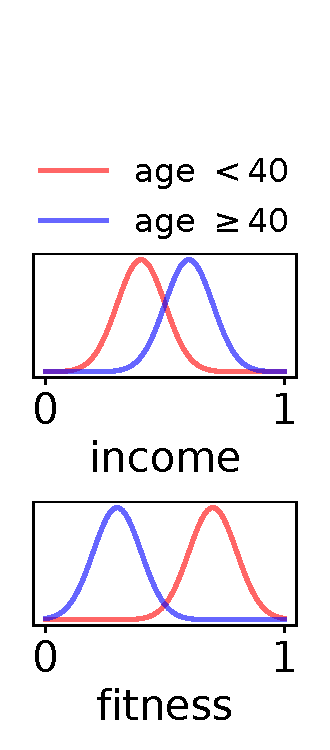
\includegraphics[scale=0.5]{figures/fairness/justicia/example.pdf}
	\end{minipage}\hspace*{-2em}
	\begin{minipage}{.35\columnwidth}
		\scalebox{0.48}{	
			\begin{tikzpicture}[x=1cm,y=1.8cm]
			\node [box, scale=1.5]                                    (p)      {fitness $\geq 0.61$};
			\node [scale=1.5, above= 0.1cm of p]  (a)    {Trained Decision Tree};
			\node [scale=1.5, box, below= of p, xshift=-2.5cm]    (a1)    {income\\ $\geq 0.29$};
			\node [scale=1.5, box, below= of p, xshift=2.5cm]     (a2)    {income $\geq 0.69$};
			\node [scale=1.5,below= of a1, xshift=-1.8cm]  (a11)    { $\hat{Y}= 1$};
			\node [scale=1.5,below= of a1, xshift=1.8cm]   (a12)    { $\hat{Y}=0 $};
			\node [scale=1.5,below= of a2, xshift=-1.8cm]  (a21)    { $\hat{Y}= 1$};
			\node [scale=1.5,below= of a2, xshift=1.8cm]  (a22)    { $\hat{Y}= 0$};
			%
			\path [line] (p) -|         (a1) node [scale=1.5,midway, above]  {Yes};
			\path [line] (p) -|         (a2) node [scale=1.5,midway, above]  {No};
			\path [line] (a1) -|       (a11) node [scale=1.5,midway, above]  {Yes};
			\path [line] (a1) -|       (a12) node [scale=1.5,midway, above]  {No};
			\path [line] (a2) -|       (a21) node [scale=1.5,midway, above]  {Yes};
			\path [line] (a2) -|       (a22) node [scale=1.5,midway, above]  {No};
			\end{tikzpicture}}
	\end{minipage}%
	\caption[A decision tree classifier on sensitive and non-sensitive features]{A trained decision tree to learn eligibility for health insurance using age-dependent fitness and income indicators.}\label{fairness_justicia_fig:fair_example}%\vspace*{-2em}
\end{figure}


\subsubsection{Fair Machine Learning} Statistical discrimination caused by classifiers has motivated researchers to formulate several definitions of fairness and develop associated algorithms to mitigate bias. \red{In this chapter, we focus on a popular concept of fairness, known as group fairness.}\change{Add causal fairness here}  Existing group fairness metrics mostly belong to three categories: \textit{independence}, \textit{separation}, and \textit{sufficiency}~\cite{mehrabi2019survey}. Independence metrics, such as demographic parity, statistical parity, and group parity, try and ensure the outcomes of a classifier to be independent of the groups that the individuals belong to~\cite{feldman2015certifying,dwork2012fairness}. Separation metrics\unsure{Incorrect definition}, such as equalized odds, define a classifer to be fair if the probability of getting the same outcomes for different groups are same~\cite{hardt2016equality}. Sufficiency metrics\unsure{Check definition}, such as counterfactual fairness, constrain the probability of outcomes to be independent of individual's sensitive data given their identical non-sensitive data~\cite{kusner2017counterfactual}.

In Figure~\ref{fairness_justicia_fig:fair_example}, independence is satisfied if the probability of getting insurance is same for both the age groups. Separation is satisfied if the number of `actually' (ground-truth) ineligible and eligible people getting the insurance are same. \red{Sufficiency is satisfied if the eligibility is independent of their age given their features are the same}\unsure{check}. Thus, we see that the metrics of fairness can be contradictory and complimentary depending on the application and the data~\cite{corbett2018measure}. To this end, different algorithms have also been devised to ensure one or multiple of the fairness definitions. These algorithms try to rectify and mitigate the bias in the data and thus in the classifier in three ways: \textit{pre-processing} the data~\cite{kamiran2012data,zemel2013learning,calmon2017optimized}, \textit{in-processing} the classifier~\cite{zhang2018mitigating}, and \textit{post-processing} the outcomes of a classifier~\cite{kamiran2012decision,hardt2016equality}.

\subsubsection{Fairness Verifiers} Due to the abundance of fairness metrics and difference in algorithms to achieve them, it has become necessary to verify different fairness metrics over datasets and algorithms. 

In order to verify fairness as a model property on a dataset, verifiers like \textit{FairSquare}~\cite{albarghouthi2017fairsquare} and \textit{VeriFair}~\cite{bastani2019probabilistic} have been proposed. 
%FairSquare verifies demographic parity and individual fairness as a numerical integration problem for a specific program semantics.
%VeriFair translates fairness metrics to an enumeration problem of a specified Boolean syntax.
%These papers operate for a specific Boolean sensitive feature.
These verifiers are referred to as {\em distributional verifiers} owing to the fact that their inputs are a probability  distribution of the features in the dataset and a classifier of a suitable form, and their objective is to verify fairness with respect to the distribution and the classifier.
Though FairSquare and VeriFair are robust and have asymptotic convergence guarantees, we observe that they scale up poorly with the size of inputs and also do not generalize to non-Boolean and compound sensitive features.
In contrast to the distributional verifiers, another line of work, referred to as sample-based verifiers, has focused on the design of testing methodologies  on a given fixed data sample~\cite{galhotra2017fairness,aif360-oct-2018}. 
Since sample-based verifiers are dataset-specific, they generally do not provide robustness over the distribution.


%\blue{Other papers: Probabilistic Verification of Fairness Properties via	Concentration, Verifying Individual Fairness in Machine Learning Models~\cite{john2020verifying}}
Thus, a \textit{unified formal framework} to verify \textit{different fairness metrics} of a classifer, which is \textit{scalable}, capable of \textit{handling compound protected groups}, \textit{robust} with respect to the test data, and \textit{operational on real-life} datasets and fairness-enhancing algorithms, is missing in the literature.

\subsubsection{Our Contribution.} From this vantage point, \textit{we propose to model verifying different fairness metrics as a Stochastic Boolean Satisfiability (SSAT) problem}~\cite{littman2001stochastic}. SSAT was originally introduced by ~\cite{papadimitriou1985games} to model {\em games against nature}. In this work, we primarily focus on reductions to the exist-random quantified fragment of SSAT, which is also known as E-MAJSAT~\cite{littman2001stochastic}.   SSAT is a conceptual framework that has been employed to capture several fundamental problems in artificial intelligence such as computation of maximum a posteriori (MAP) hypothesis~\cite{fremont2017maximum},  propositional probabilistic planning~\cite{majercik2007appssat},  and circuit verification~\cite{lee2018towards}. Furthermore, our choice of SSAT as a target formulation is motivated by the recent algorithmic progress that has yielded efficient SSAT tools~\cite{lee2017solving,lee2018solving}.



%We formulate SSAT encodings of the fairness verification problems and two methods to evaluate them in order to verify independence and separation metrics for any supervised learning \red{algorithm} using a unified scheme.
%Our encodings not only allow us to compute for non-Boolean and compound sensitive features but also to scale significantly better than existing formal verifiers. 
%We perform experimental analysis for multiple fairness metrics, datasets, and \red{algorithm}s to instantiate the efficiency and effectiveness of our approach.

Our contributions are summarised below:
\begin{itemize}
	\item We propose a unified SSAT-based approach, {\justicia}, to verify independence and separation metrics of fairness for different datasets and classifiers.
	%\item \blue{{\justicia} measures fairness metrics for pre-, in-, and post-processing \red{algorithm}s with respect to the data  generating distribution}.
	\item Unlike previously proposed formal distributional verifiers, namely FairSquare and VeriFair, {\justicia} verifies fairness for compound and non-Boolean sensitive features.%, and also \red{separation metrics}.
	\item Our experiments validate that our method is more accurate and scalable than the distributional verifiers, such as FairSquare and VeriFair, and more robust than the sample-based empirical verifiers, such as AIF360.
	\item We prove a finite-sample error bound on our estimated fairness metrics which is stronger than the existing asymptotic guarantees.
\end{itemize}

It is worth remarking that significant advances in artificial intelligence bear testimony to the right choice of formulation, for example, formulation of planning as satisfiability (SAT)~\cite{kautz1992planning}. In this context, we view that formulation of fairness as SSAT has potential to spur future work from both the modeling and encoding perspective as well as core algorithmic improvements in the underlying SSAT solvers.  

\iffalse
With this growing set of \red{algorithm}s and definitions, it has become important to measure and verify fairness and bias of different \red{algorithm}s and datasets. 
One popular approach is to use specific test dataset to compute the related statistical quantities and to certify fairness for that specific test dataset.
AIF360~\cite{aif360-oct-2018} provides a unified framework to implement multiple \red{algorithm}s and to measure their fairness depending on such test datasets.
Though this method of verification works for a specified datasets, such verifiers do not explain how much a fairness measure depends on which sensitive feature and is not robust to the selection of test dataset and its size.
\fi
				\section{Background: Fairness and SSAT}
\label{fairness_justicia_sec:preliminaries}

In this section, we define different fairness metrics for a supervised learning problem. Following that, we discuss Stochastic Boolean Satisfiability (SSAT) problem.

\subsection{Fairness Metrics for Machine Learning}\label{fairness_justicia_sec:fairness}


We consider\footnote{{We represent sets/vectors by bold letters, and the corresponding distributions by calligraphic letters. We express random variables in uppercase, and an assignment of a random variable in lowercase.}} a dataset $ \mathbf{D} $ as a collection of triples $ (\nonsensitive, \sensitive, Y) $ generated from an underlying distribution $\mathcal{D}$. $ \nonsensitive \triangleq \{X_1, \dots, X_{\numnonsensitive}\} $ are non-sensitive features whereas $ \sensitive \triangleq \{A_1, \dots, A_{\numsensitive}\} $ are categorical sensitive features.  $Y \in \{0,1\}$ is the binary label (or class) of $(\nonsensitive,\sensitive)$. Each non-sensitive feature $ X_i$ is sampled from a continuous probability distribution {$ \mathcal{X}_i $}, and each sensitive feature $ A_j \in \{0, \dots, N_j\}  $ is sampled from a discrete probability distribution {$ \mathcal{A}_j $}. We use $ (\mathbf{x}, \mathbf{a}) $ to denote the feature-values of  $ (\nonsensitive, \sensitive) $.  For sensitive features, a valuation vector $ \mathbf{a} = [a_1, .., a_{\numsensitive}] $ is called a \textit{compound sensitive group}. For example, consider $ \sensitive = $ \{race, sex\} where race $ \in $ \{Asian, Color, White\} and sex $ \in $ \{female, male\}. Thus $ \mathbf{a} = $ [Asian, female]  is a compound sensitive group. 
We represent a binary classifier trained on the dataset $\mathbf{D}$ as $\alg: (\nonsensitive, \sensitive) \rightarrow \hat{Y} $. Here, $\hat{Y} \in \{0,1\}$ is the predicted class of $ (\nonsensitive, \sensitive) $.



As we illustrated in Example~\ref{fairness_justicia_example:intro}, a classifier $\alg$ that solely optimizes accuracy, i.e., the average number of times $\hat{Y} = Y$, may discriminate certain compound sensitive groups over others~\cite{chouldechova2020snapshot}. In the following, we describe two well-known fairness definitions verified by {\justicia}: group fairness and causal fairness. To this end, we use $ f(\alg, \mathcal{D}) $ to quantify the fairness of the classifier $ \alg $ provided the distribution of features $ \mathcal{D} $. More specifically,  {\justicia} verifies fairness metrics where $ f(\alg, \mathcal{D}) $ depends on the conditional Positive Predictive Value (PPV) of the classifier, denoted by $ \Pr[\hat{Y} = 1 | \mathsf{C}] $. Henceforth, each fairness metric is identified by the particular choice of the conditional $ \mathsf{C} $, as discussed next.

\subsubsection{Group Fairness.} Group fairness is categorized into three families: independence, separation and sufficiency, of which {\justicia} verifies independence and separation metrics. 
The independence metrics state that the predicition of the classifier should be independent of compound sensitive groups. Formally, independence notion specifies an equal PPV across all sensitive groups for a classifier, i.e., $\Pr[\hat{Y} =1 | \mathbf{A} =  \mathbf{a}]  =  \Pr[\hat{Y} =1 | \mathbf{A} =  \mathbf{a}'] , \forall \mathbf{a}, \mathbf{a}' \in \sensitive$.
Since satisfying independence exactly is hard, relaxations of independence fairness metrics, such as \textit{disparate impact} and \textit{statistical parity}, are proposed in the literature~\cite{dwork2012fairness,feldman2015certifying}.

\textit{Disparate impact} (DI) measures the ratio of PPVs between the most favored group and least favored group, and prescribe it to be close to $1$~\cite{feldman2015certifying}.  Formally, the disparate impact of a classifier is 
\[
f_{\mathsf{DI}}(\alg, \mathcal{D}) \triangleq \frac{\min_{\mathbf{a}} \Pr[\hat{Y} =1 | \mathbf{A} =  \mathbf{a}]}{\max_{\mathbf{a}} \Pr[\hat{Y} =1 | \mathbf{A} =  \mathbf{a}]},
\]
where the subscript of $ f $ denotes the corresponding fairness metric.

Another popular relaxation of independence metrics  is \textit{statistical parity} (SP) that measures the maximum difference of PPVs among sensitive groups, and prescribe this quantity to be near zero. Thus, the statistical parity of  a classifier is 
\[ f_{\mathsf{SP}}(\alg, \mathcal{D}) \triangleq \max_{\mathbf{a}}\Pr[\hat{Y} =1 | \mathbf{A} = \mathbf{a}] - \min_{\mathbf{a}}\Pr[\hat{Y} =1 | \mathbf{A} = \mathbf{a}]. \]



In the \textit{separation (or classification parity)} notion of fairness, the predicted label $\hat{Y}$ of a classifier is independent of the sensitive features $\sensitive$ given the class labels $Y$. In case of binary classifiers, a popular separation metric is \textit{equalized odds} (EO)~\cite{hardt2016equality} that computes the maximum difference of false positive rates \red{(FPR)} and true positive rates \red{(TPR)} conditioned on sensitive groups. Formally,  for $ Y \in \{0,1\} $,  the equalized odds of a classifier is defined as 
\begin{align*}
f_{\mathsf{EO}}(\alg, \mathcal{D})  \triangleq \max(&\max_{\mathbf{a}}\Pr[\hat{Y} =1 | \mathbf{A} = \mathbf{a}, Y = 0] - \min_{\mathbf{a}}\Pr[\hat{Y} =1 | \mathbf{A} = \mathbf{a}, Y = 0], \\
&\max_{\mathbf{a}}\Pr[\hat{Y} =1 | \mathbf{A} = \mathbf{a}, Y = 1] - \min_{\mathbf{a}}\Pr[\hat{Y} =1 | \mathbf{A} = \mathbf{a}, Y = 1]). 
\end{align*}


\subsubsection{Path-specific Causal Fairness.}
Let $ \mathbf{a}_{\max}  \triangleq \argmax_{ \mathbf{a}} \Pr[\hat{Y} =1 |\mathbf{A}=  \mathbf{a}] $. We consider mediator features $ \mediator \subseteq \nonsensitive $ sampled from the conditional distribution $ {\mathcal{Z}_{|\mathbf{A} = \mathbf{a}_{\max}}} $. This emulates the fact that mediator variables have the same sensitive features $ \mathbf{a}_{\max} $.   To this end, the path-specific causal fairness of a classifier is \[
 f_{\mathsf{PCF}}(\alg, \mathcal{D}) \triangleq \max_{\mathbf{a}}\Pr[\hat{Y} = 1 | \sensitive =  \mathbf{a}, \mediator] - \min_{\mathbf{a}} \Pr[\hat{Y} = 1 | \sensitive = \mathbf{a}, \mediator ].
\]



Therefore, PCF constrains that $ \hat{Y} $ is not directly dependent of $ \sensitive $ while $ \sensitive $ may indirectly affects $ \hat{Y} $ only through $ \mediator $. PCF is a variation of counterfactual fairness and causal fairness without mediator features~\cite{bastani2019probabilistic}. 




\begin{example}
	Following~\cite{bastani2019probabilistic}, we consider a classifier that decides the hiring of employees based on three features: gender (sensitive), years of experience (non-sensitive), and college-participation (mediator). It is practical to consider that gender $ \in $ \{male, female\} can affect the college-participation of individuals, and all three features are determining factors for the hiring process. Let `male' be the most favored group by the classifier, for instance. Path-specific causal fairness (PCF) ensures that a female candidate should be given a job offer with similar probability as a male candidate (by constraining $ \epsilon \approx 0 $). She,  however,  went to (participated in) college as if she were a male candidate while other non-mediator features such as  `years of experience' are the same.  Therefore, PCF measures the effect of gender on job offer, but ignores the effect of gender on whether candidates went to college.
\end{example}	



\paragraph{Fairness Certification.} We certify the fairness of a classifier by comparing $ f(\alg, \mathcal{D}) $ with a fairness threshold, denoted by $ \epsilon \in [0,1] $, which quantifies the desired level of fairness. In particular, a classifier is $ \epsilon $-fair with respect to statistical parity, equalized odds, or path-specific causal fairness if and only if $ f(\alg, \mathcal{D}) \le \epsilon $. In contrast, a classifier satisfies $(1 - \epsilon)$-disparate impact  if and only if $ f(\alg, \mathcal{D}) \ge 1 - \epsilon $. In all above fairness metrics, a lower value of $ \epsilon $ refers to higher fairness of the classifier.






\subsection{Stochastic Boolean Satisfiability (SSAT)}\label{fairness_justicia_sec:ssat}
Let $\mathbf{B}  = \{\bool_1, \dots, \bool_m\}  $ be a set of Boolean variables. A \textit{literal} is a variable $ \bool_i $ or its complement $ \neg \bool_i $. 
A propositional formula $\phi$ defined over $\mathbf{B}$ is in \textit{Conjunctive Normal Form (CNF)} if $\phi$   is  a conjunction of clauses and each clause is a disjunction of literals. 
%\red{DNF (disjunctive normal form) is the  complement of CNF where  the formula is a disjunction of clauses and each clause is  a conjunction of literals.} 
Let $ \sigma $ be an assignment to the  variables $ \bool_i \in \mathbf{B} $  such that $ \sigma(\bool_i) \in \{1, 0\} $. The propositional  \textit{satisfiability} problem (SAT) finds an assignment $ \sigma $ to all $ \bool_i \in  \mathbf{B} $ such that the formula $ \phi $ is evaluated to be $1$ (equivalently, true). 
In contrast to the SAT problem, the \textit{Stochastic Boolean Satisfiability} (SSAT) problem~\cite{littman2001stochastic} is computes the  probability of the satisfaction of the formula $\phi$ defined on \textit{quantified} Boolean variables. 
An SSAT formula is of the form
\begin{equation}\label{fairness_justicia_eq:ssat}
\Phi = Q_1\bool_1, \dots, Q_m \bool_m,\; \phi, 
\end{equation}
where $ Q_i \in \{\exists, \forall, \R^{p_i}\} $ is either of the existential ($\exists$), universal ($\forall$), or randomized ($\R^{p_i}$) quantifiers on $\bool_i$ and $\phi$ is a quantifier-free CNF formula. In case of a randomized quantifier $ \R^{p_i} $, $ p_i \in [0,1] $ is the probability of $ \bool_i $ being assigned to $ 1 $. In the SSAT formula $ \Phi $, the quantifier part $ Q_1\bool_1, \dots, Q_m \bool_m $ is known as the \textit{prefix} of the formula $ \phi $.  Let $ \bool $ be the outermost variable in the prefix. The semantics of SSAT formulas are defined recursively in the following.
\begin{enumerate}
	\item $ \Pr[\text{true}] = 1 $,  $ \Pr[\text{false}] = 0 $, 
	\item $ \Pr [\Phi] = \max_{\bool} \{\Pr[\Phi|_{\bool}], \Pr[\Phi|_{\neg \bool}]\}$ if $ \bool $ is existentially quantified ($ \exists $), 
	\item $ \Pr [\Phi] = \min_{\bool} \{\Pr[\Phi|_{\bool}], \Pr[\Phi|_{\neg \bool}]\} $ if $ \bool $ is universally quantified ($ \forall $), 
	\item $ \Pr [\Phi] = p\Pr[\Phi|_{\bool}] + (1-p) \Pr[\Phi|_{\neg \bool}] $ if $ \bool $ is randomized quantified ($\R^{p}$) with probability $p$ of being $\text{true}$,
\end{enumerate}
where $ \Phi|_{\bool} $ and $ \Phi|_{\neg \bool} $ denote the SSAT formulas derived by eliminating the outermost quantifier of $ \bool $  by substituting the value of $ \bool $ in the formula $ \phi $ with $ 1 $ and $ 0 $, respectively. In this paper, we focus on two specific types of SSAT formulas:  \textit{random-exist} (RE) SSAT and \textit{exist-random} (ER) SSAT. In the ER-SSAT (resp.\ RE-SSAT) formula, all existentially (resp.\ randomized) quantified variables are followed by randomized (resp.\ existentially) quantified variables in the prefix.


\begin{remark}
	ER-SSAT problem is $\mathrm{NP}^{\mathrm{PP}}$-hard whereas RE-SSAT problem is $\mathrm{PP}^{\mathrm{NP}}$-complete~\cite{littman2001stochastic}.
\end{remark}



The problem of SSAT and its variants have been pursued by theoreticians and practitioners for over three decades~\cite{majercik2005dc,fremont2017maximum,huang2006combining}. We refer the reader to~\cite{lee2017solving,lee2018solving} for detailed survey. It is worth remarking that the past decade has witnessed a significant performance improvements of SSAT solving, thanks to the close integration of techniques from SAT solving with advances in weighted model counting~\cite{sang2004combining,chakraborty2013scalable,chakraborty2014distribution}. 




				\section{{\justicia}: An SSAT-based Fairness Verifier}
\label{fairness_justicia_sec:framework}
In this section, we present the primary contribution of this chapter, {\justicia}, which is an SSAT-based framework for verifying group and causal fairness metrics. Given a binary classifier $\alg$, a probability distribution over features $(\nonsensitive,\sensitive,Y) \sim \mathcal{D} $, and a target fairness metric $ f(\alg, \mathcal{D}) $, our goal is to estimate the fairness $ f(\alg, \mathcal{D}) $ of the classifier $ \alg $ given the distribution $ \mathcal{D} $ according to the fairness definition. Additionally, if a fairness threshold $ \epsilon \in [0,1] $ is provided, {\justicia} verifies whether the classifier is $ \epsilon $-fair by comparing $ f $ with $ \epsilon $. In {\justicia}, we focus on classifiers that can be represented as a CNF formula defined over a set of Boolean variables. Additionally, for each variable, we query the distribution $ \mathcal{D} $ to derive the marginal probability of the variable to be assigned to $ 1 $. In this section, we discuss two equivalent approaches for fairness verification based on SSAT-based encodings: \emph{enumeration} approach and \emph{inference} approach. In both approaches, we verify fairness with the presence of compound sensitive groups.  We then provide a theoretical analysis for a high-probability error bound on the fairness metric and conclude with an extension of {\justicia} in practical settings.




\iffalse
In this section, we present the main contribution of this paper, {\justicia}, which is an SSAT framework for verifying independence and separation metrics of fairness. 
We first state the problem formally in Section~\ref{fairness_justicia_sec:problem_statement}. 
To verify fairness metrics in compound sensitive groups, we discuss an enumeration approach in Section~\ref{fairness_justicia_sec:enumeration_ssat} and an equivalent but more efficient learning approach in Section~\ref{fairness_justicia_sec:learn_ssat}. 
We conclude this section by proposing a conditional distribution based enumeration for compound sensitive groups in Section~\ref{fairness_justicia_sec:cond_ssat}. 


\subsection{Problem Statement}
\label{fairness_justicia_sec:problem_statement}
Given a binary classifier $\alg$ and a probability distribution over dataset $(X,A,Y) \sim \mathcal{D} $, our goal is to verify whether $\alg$ achieves independence and separation metrics with respect to the distribution $\mathcal{D}$. We  focus on a classifier that can be translated to a CNF formula of Boolean variables $\mathbf{B} $. 
The probability $ p_i $ of $\bool_i \in \mathbf{B}$ being assigned to $1$ is induced by the data generating distribution $\mathcal{D}$. 
In our contribution, we reduce the verification problem to solving appropriately designed SSAT instances.
\fi 

\subsection{Enumeration Approach  using RE-SSAT encoding}
\label{fairness_justicia_sec:enumeration_ssat}
In order to estimate $ f(\alg, \mathcal{D}) $ in the enumeration approach, the key idea  is to compute the conditional probability of positive prediction of the classifier, $\Pr[\widehat{Y} = 1 | \sensitive = \mathbf{a}]$, for the compound sensitive group $\sensitive = \mathbf{a}$ by solving an appropriately designed SSAT formula.  For simplicity, we  initially make assumptions on the classifier $ \alg $ and discuss practical relaxations later in this section.  We first assume $\alg$ to be represented as a CNF formula, denoted by $\phi_{\widehat{Y}}$, such that the prediction $ \widehat{Y} = 1 $ when $ \phi_{\widehat{Y}}$ is satisfied and  $\widehat{Y} =0$ otherwise. Additionally, all features $ \nonsensitive \cup \sensitive $ are assumed to be Boolean variables.  Finally, we consider independence probability assumption of non-sensitive features $ \nonsensitive $, where $p_i \triangleq \Pr[X_i = 1] $ is the marginal probability of $ X_i $. 



Now, we define an RE-SSAT formula $\Phi_{\mathbf{a}}$ to compute the conditional probability $\Pr[\widehat{Y} = 1 | \sensitive = \mathbf{a}]$ using the probability of satisfaction of $\Phi_{\mathbf{a}}$. In the prefix of $ \Phi_{\mathbf{a}} $,  all non-sensitive features $ \nonsensitive $ are assigned randomized quantifiers and they are followed by sensitive features $ \sensitive $ with existential quantifiers.  In addition, the CNF formula $ \phi $ in the SSAT formula $ \Phi_{\mathbf{a}} $ is constructed such that $ \phi $ encodes the event inside the target probability $ \Pr[\widehat{Y} = 1 | \sensitive = \mathbf{a}] $. In order to specify the sensitive group $ \sensitive = \mathbf{a} $, we take the conjunction of the Boolean variables in $ \sensitive $ that symbolically specifies the compound sensitive group $ \sensitive = \mathbf{a} $. For example, let us consider two sensitive features: race $ \in $ \{White, Colour\} and sex $ \in $ \{male, female\} by Boolean variables $ R $ and $ S $,  respectively. Hence, the compound groups $ [\textrm{White}, \textrm{male}] $ and $[\textrm{Colour}, \textrm{female}]$ are represented by $ R \wedge S $ and $ \neg R \wedge \neg S $, respectively. Thus, the RE-SSAT formula for computing the probability  $ \Pr[\widehat{Y} = 1 | \sensitive = \mathbf{a}] $ is
\begin{equation}	\label{fairness_justicia_eq:re}
\begin{split}
	\Phi_{\mathbf{a}} := \underbrace{\R^{p_{1}}X_1, \dots, \R^{p_{\numnonsensitive}}X_{\numnonsensitive}}_{\text{non-sensitive features}},  &\underbrace{\exists A_1,\dots, \exists A_{\numsensitive}}_{\text{sensitive features}},
\phi_{\widehat{Y}} \wedge (\sensitive =\mathbf{a}).\notag
\end{split}
\end{equation}
In the RE-SSAT formula $ \Phi_{\mathbf{a}} $, existentially quantified variables  $ \{A_1, \dots, A_{\numsensitive}\} $ are assigned Boolean values  according  to the constraint $ \sensitive =\mathbf{a} $.\footnote{An RE-SSAT formula becomes an R-SSAT formula when the assignment to the existential variables are fixed.} Next,  an SSAT solver computes the probability $ \Pr[\Phi_{\mathbf{a}}] $ by considering the random values of $ \{X_1, \dots, X_{\numnonsensitive}\} $ while fixing the assignment of $ \{A_1, \dots, A_{\numsensitive}\} $. Therefore, $ \Pr[\Phi_{\mathbf{a}}] $ equals the conditional probability of positive prediction of the classifier, $ \Pr[\widehat{Y} = 1 | \sensitive = \mathbf{a}] $, for the sensitive group $ \sensitive = \mathbf{a} $. 

For simplicity, we have described the computation of conditional probability $ \Pr[\widehat{Y} = 1 | \sensitive = \mathbf{a}] $ without considering the correlation among sensitive and non-sensitive features. In reality, correlation exists among these features (for a detailed study on feature correlations in fairness verification, we refer to Chapter~\ref{chapter:fvgm}). As a result, non-sensitive features may have different conditional distributions for different sensitive groups. For a non-sensitive feature $ X_i $, we incorporate its conditional probability in the RE-SSAT encoding by setting $ p_i = \Pr[X_i = 1| \sensitive =\mathbf{a}] $ instead of the independent probability $\Pr[X_i = 1]$. Next, we illustrate this enumeration approach in Example~\ref{fairness_justicia_example:re_ssat}.
%This relaxes the independence requirement.

\begin{example}[RE-SSAT encoding]
	\normalfont
	\label{fairness_justicia_example:re_ssat}
	We illustrate the RE-SSAT encoding for calculating the probability of positive prediction for the sensitive group age $ \ge 40 $ in the decision tree of Figure~\ref{fairness_justicia_fig:fair_example}. We assign three Boolean variables $ F,I,J $ for three nodes in the decision tree, where literal $ F,I,J $ denote fitness $ \ge 0.61 $, income $ \ge 0.29 $, and income $ \ge 0.69 $, respectively. We consider another Boolean variable $A$  where the literal $ A $ represents the sensitive group age $ \ge 40 $ and $ \neg A $ denotes age $ < 40 $. Thus, the CNF formula  for the decision tree is $ (\neg F \vee I) \wedge (F \vee J) $. From the distribution in Figure~\ref{fairness_justicia_fig:fair_example}, we get $ \Pr[F] = 0.41, \Pr[I] = 0.93 $, and $ \Pr[J] = 0.09 $. Given this information, we calculate the probability of positive prediction for the sensitive group age $ \ge 40 $ by solving the following RE-SSAT formula:
	
	\begin{equation}
	\Phi_A := \R^{0.41}F, \R^{0.93}I, \R^{0.09}J, \exists A, \; (\neg F \vee I) \wedge (F \vee J) \wedge A.\notag
	\end{equation}
	
	From the solution to this SSAT formula, we get $ \Pr[\Phi_A] = 0.43 $. Similarly, to calculate the probability of positive prediction for the group age $ < 40 $, we replace the unit clause\footnote{A unit clause is a clause with a single literal.} $ A $ with $ \neg A $ in the CNF formula in $ \Phi_A $ and construct another SSAT formula $ \Phi_{\neg A} $. 
	
	\[ \Phi_{\neg A} := \R^{0.41}F, \R^{0.93}I, \R^{0.09}J, \exists A, \; (\neg F \vee I) \wedge (F \vee J) \wedge \neg A \]
	
	For $ \Phi_{\neg A} $, the solution $ \Pr[\Phi_{\neg A}] = 0.43 $ is similarly derived from an SSAT solver. 
	Therefore, if $\Pr[F], \Pr[I], \Pr[J]$ are computed independently of the sensitive feature $A$, both age groups demonstrate equal probability of positive prediction as the sensitive feature is not explicitly present in the classifier. 

	However, there is an implicit bias in the data distribution for different sensitive groups and the classifier unintentionally learns it. To capture this implicit bias, we calculate conditional probabilities  $ \Pr[F|A] = 0.01, \Pr[I|A] = 0.99 $, and $ \Pr[J|A] = 0.18 $ from the distribution for group age $ \ge 40 $ in Figure~\ref{fairness_justicia_fig:fair_example}. Providing the conditional probabilities, we construct a modified SSAT formula $\Phi'_A $ and compute $ \Pr[\Phi'_A] = 0.18 $ for age $ \ge 40 $. 
	
	\begin{equation}
	\Phi'_A := \R^{0.01}F, \R^{0.99}I, \R^{0.18}J, \exists A, \; (\neg F \vee I) \wedge (F \vee J) \wedge A\notag
	\end{equation}
	
	For the sensitive group age $ < 40 $,  we similarly obtain $ \Pr[F|\neg A] = 0.82, \Pr[I|\neg A] = 0.88 $, $ \Pr[J|\neg A] = 0.01 $, construct the modified formula $ \Phi'_{\neg A} $ and get  $ \Pr[\Phi'_{\neg A}] = 0.72 $. 

	\[ \Phi'_{\neg A} := \R^{0.82}F, \R^{0.88}I, \R^{0.01}J, \exists A, \; (\neg F \vee I) \wedge (F \vee J) \wedge \neg A \]	

	In the later case with correlations among sensitive and non-sensitive features, the RE-SSAT encoding detects the discrimination of the classifier among different sensitive groups, where the classifier is more biased towards the younger group with age $ < 40 $ than the elderly group with age $ \ge 40 $.
	
	

	
	
%	An astute reader would observe that $I$ and $J$ are not independent. Following~\cite{chavira2008probabilistic}, we can simply capture relationship between the variables using constraints and if needed, auxiliary variables. In this case, it suffices to add the the constraint $J \rightarrow I$. 
\end{example}

\subsubsection{Measuring Fairness Metrics}
As we compute $ \Pr[\Phi_\mathbf{a}] = \Pr[\widehat{Y} = 1 | \sensitive = \mathbf{a}] $ by solving the SSAT formula $ \Phi_\mathbf{a} $, we  use $ \Pr[\Phi_\mathbf{a}] $ to measure different fairness metrics. To this end, we compute $ \Pr[\Phi_\mathbf{a}] $ for all compound groups $\mathbf{a} \in \sensitive $ by solving an exponential number (with $ \numsensitive $) of SSAT formulas. We elaborate this enumeration approach, namely {\justiciaenum}, in Algorithm~\ref{fairness_justicia_algo:enum}  (Line~\ref{fairness_justicia_algo:justicia_enum_begin}--\ref{fairness_justicia_algo:justicia_enum_end}).

\begin{algorithm}[t!]
	\caption{\justicia: An SSAT-based Fairness Verifier}
	\label{fairness_justicia_algo:enum}
	\begin{algorithmic}[1]
		\Function{{\justiciaenum}}{$ \nonsensitive, \sensitive,\widehat{Y} $}
		\label{fairness_justicia_algo:justicia_enum_begin}
		\State $ \phi_{\widehat{Y}} := \mathsf{CNF}(\widehat{Y} = 1) $
		%\State $ p_{i} = \mathsf{CalculateProb}(X_i), \forall X_i \in X $
		\ForAll{$\mathbf{a} \in \sensitive$ }
		\State $ p_{i} \leftarrow \Pr[X_i = 1|\sensitive = \mathbf{a}], \forall X_i \in \nonsensitive $
		\State $ \phi := \phi_{\widehat{Y}} \wedge (\sensitive =\mathbf{a}) $
		\State $  \Phi_\mathbf{a} := \R^{p_{1}}X_1, \dots, \R^{p_{\numnonsensitive}}X_{\numnonsensitive}, \exists A_1,\dots, \exists A_{\numsensitive},  \phi $
		\State $ \Pr[\Phi_\mathbf{a}]  \leftarrow \mathsf{SSAT}(\Phi_\mathbf{a}) $ \Comment{returns a probability}
		\EndFor
		\State\Return $ \max_{\mathbf{a} \in \sensitive} \Pr[\Phi_{\mathbf{a}}], \min_{\mathbf{a} \in \sensitive} \Pr[\Phi_{\mathbf{a}}] $
		\label{fairness_justicia_algo:justicia_enum_end}
		\EndFunction
		\Statex
		
		
		
		\Function{{\justicialearn}}{$ \nonsensitive, \sensitive,\widehat{Y} $}
		\label{fairness_justicia_algo:justicia_learn_begin}
		\State $ \phi_{\widehat{Y}} := \mathsf{CNF}(\widehat{Y}  = 1) $
		\State $ p_{i} \leftarrow \Pr[X_i=1], \forall X_i \in \nonsensitive $
		\State $  \Phi_\mathsf{ER} := \exists A_1,\dots, \exists A_{\numsensitive}, \R^{p_{1}}X_1, \dots, \R^{p_{\numnonsensitive}}X_{\numnonsensitive}, \phi_{\widehat{Y}} $
		\State $  \Phi'_\mathsf{ER} := \exists A_1,\dots, \exists A_{\numsensitive}, \R^{p_{1}}X_1, \dots, \R^{p_{\numnonsensitive}}X_{\numnonsensitive}, \neg \phi_{\widehat{Y}} $
		\State\Return $ \mathsf{SSAT}(\Phi_\mathsf{ER}), 1 - \mathsf{SSAT}(\Phi'_\mathsf{ER}) $
		\label{fairness_justicia_algo:justicia_learn_end}
		\EndFunction
	\end{algorithmic}

\end{algorithm}


To measure the disparate impact of a classifier, we calculate the ratio between the minimum and the maximum conditional probability of positive prediction of the classifier, which are  $ \min_{\mathbf{a} \in \sensitive} \Pr[\Phi_{\mathbf{a}}] $ and $ \max_{\mathbf{a} \in \sensitive} \Pr[\Phi_{\mathbf{a}}] $, respectively. We compute statistical parity by taking the difference between $ \max_{\mathbf{a} \in \sensitive} \Pr[\Phi_{\mathbf{a}}] $ and $ \min_{\mathbf{a} \in \sensitive} \Pr[\Phi_{\mathbf{a}}] $. 


Moreover, to compute equalized odds, we call {\justicia} twice, one for the distribution $ \mathcal{D} $ conditioned on $ Y = 1  $ and another for $ Y = 0 $. In both calls, we compute $ \max_{ \mathbf{a}} \Pr[\widehat{Y} =1 | \sensitive = \mathbf{a}, Y = y ]  - \min_{ \mathbf{a}} \Pr[\widehat{Y} =1 | \sensitive = \mathbf{a}, Y = y ] $ for $ y \in \{0,1\} $ and take the  maximum difference as the value of equalized odds. 
For measuring path-specific causal fairness, we compute  $ \max_{ \mathbf{a}} \Pr[\widehat{Y} =1 | \sensitive = \mathbf{a}, \mathbf{Z}] $ and  $ \min_{ \mathbf{a}} \Pr[\widehat{Y} =1, \mathbf{Z}| \sensitive = \mathbf{a} , \mathbf{Z}] $ by conditioning the distribution $ \mathcal{D} $ by mediator features $ \mathbf{Z} $ and take their difference. Thus, {\justiciaenum} allows us to compute different group and causal fairness metrics using a unified algorithmic framework.





\subsection{Inference Approach using ER-SSAT Encoding}
\label{fairness_justicia_sec:learn_ssat}
In most practical problems, there can be exponentially many compound sensitive groups due to the combination of categorical sensitive features.  As a result, the enumeration approach may suffer from scalability issues due to an exponential number of calls to the SSAT solver. To this end, we propose an efficient SSAT encoding, where we make two SSAT calls, one for inferring the \emph{the most favored sensitive group} with the maximum conditional probability of positive prediction of the classifier and another for inferring \emph{the least favored sensitive group} with the minimum conditional probability of positive prediction of the same classifier. As discussed above, these two probabilities are sufficient to measure different group and causal fairness metrics.

\todo{End of revision}

\subsubsection{Inferring the Most Favored Sensitive Group}
In the prefix of an SSAT formula $ \Phi $, the order of quantified variables carries distinct interpretation of  $ \Pr[\Phi] $.   In an ER-SSAT formula, $ \Pr[\Phi] $ is the \textit{maximum} satisfying probability of $ \Phi $ over the optimal assignment of existentially quantified variables given the randomized quantified variables (by Semantic 2, Sec.~\ref{fairness_justicia_sec:ssat}). In this chapter, we leverage this property to compute the most favored sensitive group with the highest probability of positive prediction of the classifier. In particular, we consider the following ER-SSAT formula:

\begin{equation}
\Phi_{\mathsf{ER}} := \exists A_1,\dots, \exists A_{\numsensitive},
 \R^{p_{1}}X_1, \dots, \R^{p_{\numnonsensitive}}X_{\numnonsensitive},   \; \phi_{\widehat{Y}}.
 \label{fairness_justicia_eq:er}
\end{equation}

The CNF formula $\phi_{\widehat{Y}}$ in $ \Phi_{\mathsf{ER}} $ is the CNF translation  of the classifier $ \widehat{Y} = 1 $ without any specification of the compound sensitive group.  Therefore, as we solve $ \Phi_{\mathsf{ER}} $, we find the optimal assignment to the existentially quantified variables $ A_1 = a^{\max}_1, \dots,A_{\numsensitive} = a^{\max}_{\numsensitive} $ for which the probability of satisfaction of the ER-SSAT formula $ \Pr[\Phi_{\mathsf{ER}}] $ becomes maximum. Thus, we compute  the most favored group $ \mathbf{a}_{\max} \triangleq [ a^{\max}_1, \dots, a^{\max}_{\numsensitive} ] $ achieving the highest probability of positive prediction of the classifier. 


\subsubsection{Inferring the Least Favored Sensitive Group}
In order to infer the least favored sensitive group of the classifier, we  compute the \textit{minimum} conditional probability of positive prediction of the classifier with respect to all sensitive groups given the random values of the non-sensitive features. To this end, we  solve a `universal-random' (UR) SSAT formula with  universal quantifiers over sensitive features and randomized quantification over non-sensitive features (by Semantic 3, Sec.~\ref{fairness_justicia_sec:ssat}).
\begin{equation}
\Phi_{\mathsf{UR}} := \forall A_1,\dots, \forall A_{\numsensitive},
\R^{p_{1}}X_1, \dots, \R^{p_{\numnonsensitive}}X_{\numnonsensitive},   \; \phi_{\widehat{Y}}
\label{fairness_justicia_eq:ar}
\end{equation}
%By solving $ \Phi_{\mathsf{UR}} $, we find the optimal assignment to the universally quantified variables $ A_1 = a^{\min}_1, \dots,A_{\numsensitive} = a^{\min}_{\numsensitive} $ for which the probability of satisfaction of the UR-SSAT formula $ \Pr[\Phi_{\mathsf{UR}}] $ becomes minimum. Thus, $ \red{\mathbf{a}_{\min}} \triangleq [ a^{\min}_1, \dots, a^{\min}_{\numsensitive} ] $ becomes the least favored sensitive group achieving the lowest probability of positive prediction of the classifier. 

Solving an UR-SSAT formula raises several practical issues and thus, there is an unavailability of a UR-SSAT solver. To resolve this problem, we leverage the \textit{duality} between UR-SSAT  and ER-SSAT formulas, where we solve an UR-SSAT formula on the CNF $ \phi $ using the solution of an ER-SSAT formula on the complemented CNF $ \neg \phi $~\cite{littman2001stochastic}. More specifically, we solve the following ER-SSAT formula for finding the least favored sensitive group.

\begin{equation}
	\Phi'_{\mathsf{ER}} := \exists A_1,\dots, \exists A_{\numsensitive},
	\R^{p_{1}}X_1, \dots, \R^{p_{\numnonsensitive}}X_{\numnonsensitive},   \; \neg \phi_{\widehat{Y}}
	\label{fairness_justicia_eq:er_complement}
\end{equation}


In Lemma~\ref{fairness_justicia_thm:dual}, we discuss the duality between UR-SSAT and ER-SSAT formulas.


\begin{lemma}\label{fairness_justicia_thm:dual}
Given Eq.~\eqref{fairness_justicia_eq:ar} and~\eqref{fairness_justicia_eq:er_complement},	$ \Pr[\Phi_{\mathsf{UR}}] = 1 - \Pr[\Phi'_{\mathsf{ER}}]  $.
\end{lemma}

\begin{proof}[Proof of Lemma~\ref{fairness_justicia_thm:dual}]
	Both $ \Phi_{\mathsf{UR}} $ and $ \Phi'_{\mathsf{ER}} $ have  random quantified variables in the identical order in the prefix. According to the definition of SSAT formulas,
	\begin{equation*}
	\Pr[\Phi_{\mathsf{UR}}] = \min\limits_{a_1, \dots,a_{\numsensitive}} \Pr[\phi_{\widehat{Y}}] \text{ and } \Pr[\Phi'_{\mathsf{ER}}] = \max\limits_{a_1, \dots,a_{\numsensitive}} \Pr[\neg\phi_{\widehat{Y}}],
	\end{equation*}
	
	where $ \Pr[\phi_{\widehat{Y}}] $ and $ \Pr[\neg \phi_{\widehat{Y}}] $ are both computed for the random values of non-sensitive features $ \nonsensitive $.
	
	Therefore, we derive the following duality between ER-SSAT and UR-SSAT,
	\begin{equation}
	\begin{split}
	\Pr[\Phi'_{\mathsf{ER}}] &= \max\limits_{a_1, \dots,a_{\numsensitive}} \Pr[\neg\phi_{\widehat{Y}}]  \\
	&= \min\limits_{a_1, \dots,a_{\numsensitive}} (1 - \Pr[\phi_{\widehat{Y}}])\\
	&= 1 - \min\limits_{a_1, \dots,a_{\numsensitive}}  \Pr[\phi_{\widehat{Y}}]\\
	&= 1 - \Pr[\Phi_{\mathsf{UR}}].\notag
	\end{split}
	\end{equation}
\end{proof}


As we solve $\Phi'_{\mathsf{ER}}$, we obtain the optimal assignment to the sensitive features $\mathbf{a}_{\min} \triangleq [a^{min}_1, \dots, a^{min}_{\numsensitive}]$ that maximizes $\Phi'_{\mathsf{ER}}$.  If $ p $ is the maximum satisfying probability of $ \Phi'_{\mathsf{ER}} $, then according to Lemma~\ref{fairness_justicia_thm:dual}, $ 1 - p $ is the minimum satisfying probability of $ \Phi_{\mathsf{UR}} $;  which is also the minimum probability of positive prediction of the classifier. We present the algorithm for the inference approach, namely {\justicialearn} in Algorithm~\ref{fairness_justicia_algo:enum} (Line~\ref{fairness_justicia_algo:justicia_learn_begin}--\ref{fairness_justicia_algo:justicia_learn_end}).

\iffalse
\begin{algorithm}[t!]
	\caption{\justicialearn: Learning ER-SSAT Encoding}
	\label{fairness_justicia_algo:learn}
	\begin{algorithmic}[1]
		\Function{{\justicialearn}}{$ X,A,\widehat{Y} $}
		\State $ \phi_{\widehat{Y}} = \mathsf{CNF}(\widehat{Y}  = 1) $
		\State $ p_{i} = \mathsf{CalculateProb}(x_i), \forall x_i \in X $
		\State $  \Phi_\mathbf{ER} = \exists a_1,\dots, \exists a_{\numsensitive}, \R^{p_{1}}x_1, \dots, \R^{p_{\numnonsensitive}}x_{\numnonsensitive}. \; \phi_{\widehat{Y}} $
		\State $  \Phi'_\mathbf{ER} = \exists a_1,\dots, \exists a_{\numsensitive}, \R^{p_{1}}x_1, \dots, \R^{p_{\numnonsensitive}}x_{\numnonsensitive}. \; \neg \phi_{\widehat{Y}} $
		\State \Return $ \mathsf{SSAT}(\Phi_\mathbf{ER}), 1 - \mathsf{SSAT}(\Phi'_\mathbf{ER}) $
		\EndFunction
	\end{algorithmic}
\end{algorithm}
\fi

In the ER-SSAT formula in Eq.~\eqref{fairness_justicia_eq:er_complement}, we need to negate the classifier $ \phi_{\widehat{Y}} $ to another CNF formula $ \neg \phi_{\widehat{Y}} $. The na\"ive approach of negating one CNF to another CNF generates an exponential number of new clauses. Here, we apply Tseitin transformation for the negation, which increases the number of clauses linearly while introducing a linear number of new variables~\cite{tseitin1983complexity}. As an alternative approach, we directly encode the binary classifier $\alg$ for the negative class label $\widehat{Y} = 0$ as a CNF formula and pass it to $\Phi'_{\mathsf{ER}} $, whenever it is possible. The latter approach is generally more efficient than the former approach as the resulting CNF is often smaller.  






\begin{example}[ER-SSAT encoding]
	\normalfont
	\label{fairness_justicia_example:er_ssat}
	Here, we illustrate the ER-SSAT encoding for inferring the most favored and the least favored sensitive group of a classifier in the presence of compound sensitive groups. As the example in Figure~\ref{fairness_justicia_fig:fair_example} is degenerate for this purpose, we introduce another Boolean sensitive feature `sex' $ \in $ \{male, female\}. We consider a Boolean variable $ S $ for sex where the literal $ S $ denotes sex = male. With this new sensitive feature, let the classifier be  $\alg \triangleq (\neg F \vee I \vee S) \wedge (F \vee J)$, where variables corresponding to sensitive features $ F,I$, and  $J $ have same distributions as discussed in Example~\ref{fairness_justicia_example:re_ssat}. Hence, we obtain the following ER-SSAT formula of $\alg$ to infer the most favored sensitive group:
	
	\[ \Phi_{\mathsf{ER}} =  \exists S,\exists A, \R^{0.41}F, \R^{0.93}I, \R^{0.09}J, \; (\neg F \vee I \vee S) \wedge (F \vee J).
	\]
	
	As we solve $ \Phi_{\mathsf{ER}} $, we infer that the optimal assignment to the existential variables $ \sigma(S) = 1, \sigma(A) = 0$, which implies that `male individuals with age $ < 40 $' is the most favored group with probability of positive prediction computed as $ \Pr[\Phi_{\mathsf{ER}}] = 0.46$. Similarly, to infer the least favored group, we negate the CNF translation of the classifier $\alg$ to obtain the following ER-SSAT formula:
	
	\[\Phi'_{\mathsf{ER}} =  \exists S, \exists A, \R^{0.41}F, \R^{0.93}I, \R^{0.09}J, \; \neg((\neg F \vee I \vee S) \wedge (F \vee J)).
	\]
	
	Solving $ \Phi'_{\mathsf{ER}} $, we learn the optimal assignment $ \sigma(S) = 0, \sigma(A) = 0  $ and $  \Pr[\Phi'_{\mathsf{ER}}] = 0.57 $. Thus, `female individuals with age $ < 40 $' constitute the least favored group with probability of positive prediction as  $ 1-0.57 = 0.43$. 
	Thus, {\justicialearn} allows us to infer the most and least favored sensitive groups and the corresponding discrimination.
\end{example}



We next prove the equivalence of {\justiciaenum} and {\justicialearn} in Lemma~\ref{fairness_justicia_lm:equivalence}.

\begin{lemma}
	\label{fairness_justicia_lm:equivalence}
	Let $ \Phi_{\mathbf{a}} $ be an RE-SSAT formula for computing the probability of positive prediction of a classifier corresponding to the sensitive group $  \sensitive = \mathbf{a} $. Additionally, for the same classifer, let $ \Phi_{\mathsf{ER}} $ be an ER-SSAT formula for inferring the most favored sensitive group and $ \Phi_{\mathsf{UR}} $ be a UR-SSAT formula for inferring the least favored sensitive group.  Therefore,	$\max_{\mathbf{a} \in \sensitive} \; \Pr[\Phi_{\mathbf{a}}] = \Pr[\Phi_{\mathsf{ER}}]$   	and	$\min_{\mathbf{a} \in \sensitive} \; \Pr[\Phi_{\mathbf{a}}] = \Pr[\Phi_{\mathsf{UR}}]$.  
\end{lemma}

\begin{proof}[Proof of Lemma~\ref{fairness_justicia_lm:equivalence}] 
	It is trivial that the probability of positive prediction of the classifier for the most favored group $ \mathbf{a}_{\max} $ is the maximum computed probability of all compound groups $ \mathbf{a} \in \sensitive $. Similar argument holds for the least favored group $ \mathbf{a}_{\min} $, which obtains the minimum probability of positive prediction of the classifier among all compound groups $ \mathbf{a} \in A $.
	
	By construction of the SSAT formulas, $ \Pr[\Phi_{\mathsf{ER}}] $ and $ \Pr[\Phi_{\mathsf{UR}}] $ are the probabilities corresponding to the groups $ \sensitive = \mathbf{a}_{\max} $ and $ \sensitive = \mathbf{a}_{\min} $, respectively. Now, since $ \Pr[\Phi_{\mathbf{a}}] $ is the probability for the group $ \sensitive = \mathbf{a} $, we derive the following.
	
	\begin{equation*}
	\begin{split}
	\max_{\mathbf{a} \in \sensitive} \; \Pr[\Phi_{\mathbf{a}}] = \Pr[\Phi_{\mathsf{ER}}]
	\text{ and }
	\min_{\mathbf{a} \in \sensitive} \; \Pr[\Phi_{\mathbf{a}}] = \Pr[\Phi_{\mathsf{UR}}]
	\end{split}
	\end{equation*}
\end{proof}


\iffalse
\begin{theorem}
	For an ER-SSAT problem, the na\"ive sample complexity is given by 
	\[ k = O\left(\frac{1}{\epsilon^2} (n + \ln(1/\delta))  \right)\]
	where $\widehat{p} - p \leq \epsilon$ with probability $1-\delta$.
\end{theorem}
\red{For a simple sampling based algo after evaluating $k$ assignments, the error between estimates probability and actual probability would differ by $\epsilon$ with probability $1- 2^{n+1} e^{-2\epsilon^2 k}$. So the sample complexity of a naive algo is $k = O(\epsilon^{-2} (\log(1/\delta) + n))$.}
\fi

%\subsection{Conditionally Evaluating an SSAT Encoding}
%\label{fairness_justicia_sec:cond_ssat}


%\begin{algorithm}[t!]
%	\caption{\justiciacond: Conditional Evaluation of RE Encoding \red{Can be removed, only difference is in line 4}}
%	\begin{algorithmic}[1]
%		\Function{{\justiciacond}}{$ X,A,\widehat{Y} $}
%		\State $ \phi_{\widehat{Y}} = \mathsf{CNF}(\widehat{Y}  = 1) $
%		\ForAll{$\mathbf{a} \in A$ }
%		\State $ p_{i} = \mathsf{\blue{calculateCondProb}}(x_i, \mathbf{a}), \forall x_i \in X $
%		\State $  \Phi_\mathbf{a} = \R^{p_{1}}x_1, \dots, \R^{p_{\numnonsensitive}}x_{\numnonsensitive}, \exists A_1,\dots, \exists A_{\numsensitive}. \; \phi_{\widehat{Y}} \wedge \mathsf{CNF}(\sensitive =\mathbf{a}) $
%		\State $ \Pr[\Phi_\mathbf{a}]  = \ma
%thsf{SSAT}(\Phi_\mathbf{a}) $
%		\EndFor
%		\State \Return $ \max\limits_{\mathbf{a}} \; \Pr[\Phi_{\mathbf{a}}], \min\limits_{\mathbf{a}} \; \Pr[\Phi_{\mathbf{a}}] $
%		\EndFunction		
%	\end{algorithmic}
%\end{algorithm}

\iffalse
\red{While it is trivial to use conditional probability distribution for the RE encoding, it is not straightforward for the presented ER-encoding, which we leave as a future work. 
}
\fi

\begin{comment}
\red{Let $ \bool_i $ and $ \bool_j $ be two Boolean (non-sensitive) features and we want to encode their pair-wise correlation in {\justicia}. For an assignment to $ \bool_i, \bool_j $, we consider a new Boolean variable $ v $ and add a constraint $ v \leftrightarrow \bool_i \wedge \bool_j $ in the CNF $ \phi $ of the SSAT formula $ \Phi $. Additionally, $ v $ is given a randomized quantification in the prefix of $ \Phi $ and the probability of $ v $ is calculated as the probability of both $ \bool_i $ and $ \bool_j $ assigning to $ 1 $ in the distribution $ \mathcal{D} $. Note that, to encode the total correlation of all Boolean features, the mentioned approach introduces exponentially (with the number of features) many new variables and add an exponential number of constraints to $ \phi $ with an aim of computing a more precise satisfying probability of $ \Phi $. Optionally, one can encode the correlation among a selected set of features of interest in {\justicia}. }
\end{comment}


\subsection{Theoretical Analysis: Error Bounds}\label{fairness_justicia_sec:theory}
For practical fairness problems, we do not have access to the distribution of features rather to a finite-sample dataset. Since the input of {\justicia} is the distribution of features, we compute the distribution from the dataset. The finite-sample dataset introduces errors in the computed probabilities of randomized quantified features being assigned to $1$. These finite-sample errors in computed probabilities induce further errors in the computed probability of positive prediction of the classifier and corresponding fairness metrics. We next provide a bound on this finite-sample error.

Let us consider that $\widehat{p_i}$ is the estimated probability of a Boolean variable $ \bool_i $ being assigned to $ 1 $ from $ n $ samples, and $p_i$ is the true probability of $ \bool_i = 1 $ according to $ \mathcal{D} $. 
%If $ | p_i - \widehat{p_i}| \le \epsilon $, i.e., $ \epsilon $ additive error for small $ \epsilon \approx 0 $, we want to compute the error of probability $ p $ of the satisfaction of the SSAT formula $ \Phi $.  
Thus, the true satisfying probability $p$ of an SSAT formula $ \Phi $ is the weighted sum of all satisfying assignments of the CNF $ \phi $, $p = \sum_{\sigma^*} \prod_{L_i \in {\sigma^*}}L_i * p_i + (1 - L_i) * (1 - p_i)$, where the literal $ L_i \in \{0,1\} $ denotes either the variable $ B_i $ when $ L_i = 1 $ or its negation when $ L_i = 0 $. This probability $ p $ is estimated as $\widehat{p}$ using $n$ samples from the distribution $\mathcal{D}$ such that $\widehat{p} \leq \epsilon_0 p$ for $\epsilon_0 \geq 1$. 
%However, the true satisfying probability $ \widehat{p} $  of $ \Phi $ is 
%\[
%\widehat{p} = \sum_\sigma \prod_{\bool_i \in \sigma}\widehat{p_i}  \leq \sum_\sigma \prod_{\bool_i \in \sigma}(1 \pm \epsilon_i) p_i = \prod_{i =1}^m (1 \pm \epsilon_i) p = \epsilon_0 p
%\]
\iffalse
If we consider $\epsilon_i = \frac{\ln \epsilon_0}{2^i}$, we obtain
\begin{equation*}
\begin{split}
\prod_{i =1}^m (1 \pm \epsilon_i) &\leq \left(\frac{1}{n} \sum_{i} (1 + \epsilon_i)\right)^n \\
&= (\frac{1}{n} \sum_{i} (1+\frac{\ln \epsilon_0}{2^i})^n\\
&\leq (1  +\frac{\ln \epsilon_0}{n})^n\\
&\leq e^{\ln \epsilon_0} = \epsilon_0.\notag
\end{split}
\end{equation*}
\fi
\begin{theorem}\label{fairness_justicia_thm:sample}
	For an ER-SSAT problem, the sample complexity is given by 
	$ n = O\left((\numsensitive+ \ln(1/\delta))\frac{\ln \numnonsensitive}{\ln \epsilon_0} \right),$
	where $\frac{\widehat{p}}{p} \leq \epsilon_0$ with probability $1-\delta$ such that $\epsilon_0 \geq 1$.
\end{theorem}
\todo{Check correctness of the theorem}
%Theorem~\ref{fairness_justicia_thm:sample} states that for the prescribed number of samples the estimated disparate impact $\widehat{DI}$ and statistical parity $\widehat{SP}$ would also satisfy $\widehat{DI} \leq  \epsilon_0 DI, $ and $\widehat{SP} \leq 2\epsilon_0 SP$.
%Apply Hoeffding inequality for each term and then use Union bound for $2^n$ existential variables.
\begin{corollary}
	\label{fairness_justicia_cor:error}
	If $n$ samples are considered from the  distribution in {\justicia} such that 
	\[
	n = O\left((\numsensitive + \ln(1/\delta))\frac{\ln \numnonsensitive}{\ln \epsilon_0}\right),
	\]
	
	the estimated disparate impact    $\widehat{\mathsf{DI}}$ and statistical parity  $\widehat{\mathsf{SP}}$ satisfy, with probability $1-\delta$,
	\[
	\widehat{\mathsf{DI}} \leq  \epsilon_0 \mathsf{DI},\text{ and }  \widehat{\mathsf{SP}} \leq 2\epsilon_0 \mathsf{SP}.
	\]
\end{corollary}
\todo{Proof is wrong}


\begin{proof}[Proof of Corollary~\ref{fairness_justicia_cor:error}] 
By Theorem~\ref{fairness_justicia_thm:sample}, we get that for $n$ samples obtained from the distribution, where

$$ n \geq (\numsensitive + \ln(1/\delta))\frac{\ln \numnonsensitive}{\ln \epsilon_0},$$

the estimated probability of satisfaction of SSAT formulas for the most and least favored sensitive groups, referred as $\widehat{p}_{max}$ and  $\widehat{p}_{min}$, respectively satisfy

\begin{equation}
\widehat{p}_{max} \leq \epsilon_0 \max_{\mathbf{a} \in \sensitive} \; \Pr[\Phi_{\mathbf{a}}]
\text{ and }
\widehat{p}_{min} \leq \epsilon_0 \min_{\mathbf{a} \in \sensitive} \; \Pr[\Phi_{\mathbf{a}}].\notag
\end{equation}

with probability $ 1-\delta $.
Thus, the estimated value of disparate impact will satisfy

$$\widehat{\mathsf{DI}} \triangleq \frac{\widehat{p}_{max}}{\widehat{p}_{min}} \leq \epsilon_0  \frac{p_{max}}{p_{min}} \leq \epsilon_0 \mathsf{DI},$$

and statistical parity will satisfy 

$$\widehat{SP} \triangleq \abs{\widehat{p}_{max} - \widehat{p}_{min}} \leq  \epsilon_0  \abs{p_{max} - p_{min}} \leq \epsilon_0 SP,$$

with probability $1-\delta$.
\end{proof}


\red{This implies that given a binary classifier represented as a CNF formula and a distribution of sensitive and non-sensitive features, {\justicia} can verify independence and separation notion of fairness up to an error level $\epsilon_0$ and $2\epsilon_0$ with probability $1-\delta$. Thus, {\justicia} is a sound framework of fairness verification with high probability.}
%\red{Proof of all theorems for arxiv version}
%Use definition of $GF = p_1/p_2$.




\iffalse

\begin{corollary}[Hypothesis]
	If $k$ samples are considered in \justicia and the estimated group fairness value $\widehat{GF}$ satisfies
	\begin{equation*}
	1- e^{\epsilon_0} \leq \frac{\widehat{GF}}{GF} \leq 1 + e^{\epsilon_0}
	\end{equation*}
	with probability $1-\delta$, then
	\begin{equation*}
	k = O\left((n+ \ln(1/\delta))\frac{m + \ln m}{\ln \epsilon_0}\right).
	\end{equation*}
\end{corollary}
\fi



				\subsection{Practical Settings}
\label{sec:practical-setting}
We now relax the assumptions of {\justicia} on access to Boolean classifiers and Boolean features, and extend {\justicia} to verify fairness metrics for more practical settings of decision trees, linear classifiers, and continuous features.

\subsubsection{Extending {\justicia} to Decision Trees and Linear Classifiers. }
In the SSAT approach, we assume that the classifier $\alg$ is represented as a CNF formula.  
We extend {\justicia} beyond CNF classifiers to decision trees and linear classifiers, which are widely used in the fairness studies~\cite{zemel2013learning,raff2018fair,zhang2019faht}.
%{\color{red}In the literature of interpretable machine learning, several studies have been conducted for learning CNF classifiers in the supervised learning setting, which include but are not limited to the work of~\cite{angelino2017learning,malioutov2018mlic,ghosh19incremental}.  We leverage these techniques. (not needed)}

\textit{Binary decision trees} are trivially encoded as  CNF formulas.  In the binary decision tree, each node in the tree is considered as a literal. A \textit{path from the root to the leaf} is a conjunction of literals and thus, a \textit{clause}. The \textit{tree} itself is a disjunction of all paths and thus, a \textit{DNF (Disjunctive Normal Form)}. In order to derive a CNF of a decision tree, we first construct a DNF by including all paths terminating at leaves with negative class label ($ \hat{Y} = 0 $) and then complement the DNF to CNF using De Morgan's rule. 

\textit{Linear classifiers on Boolean features} are encoded into CNF formulas using pseudo-Boolean encoding~\cite{philipp2015pblib}. We consider a linear classifier  $ \mathbf{W}^T \mathbf{X} + b \ge 0 $ on Boolean features $ \mathbf{X} $ with weights $ \mathbf{W} \in \mathbb{R}^{|\mathbf{X}|} $ and bias $ b \in \mathbb{R} $.  We first normalize $ \mathbf{W} $ and $ b $ in $ [-1,1] $ and then round to integers so that the decision boundary becomes a pseudo-Boolean constraint~\cite{roussel2009pseudo}.  We then apply  pseudo-Boolean constraints to CNF translation~\cite{philipp2015pblib} to encode the decision boundary to CNF. This encoding usually introduces additional Boolean variables and results in large CNF. In order to generate a smaller CNF, we can trivially apply thresholding  on the weights to consider features with higher weights only. For instance, if the weight $  |w_i| \le \lambda $ for a threshold $ \lambda  \in \mathbb{R}^+$ and $ w_i \in \mathbf{W} $, we can set $ w_i = 0 $. Thus, features with lower weights (less important) do not appear in the encoded CNF.  Moreover, all introduced variables in this CNF translation are given existential ($ \exists $) quantification and they appear in the inner-most position in the prefix of the SSAT formula. Thus, the presented ER-SSAT formulas become effectively ERE-SSAT formulas.

\subsubsection{Extending to Continuous Features.}
In practical problems, features are generally real-valued or categorical but classifiers, which are naturally expressed as CNF such as~\cite{GMM20}, are generally trained on a Boolean abstraction of input features. In order to perform the Boolean abstraction, each categorical feature is one-hot encoded and each real-valued feature is discretized into a set of Boolean features~\cite{LKCL2019,GMM20}. 

For a binary decision tree, each feature, including the continuous ones, is compared against a constant at each node (except leaves) of the tree. We assign a Boolean variable to each node (except leaves), where the $ \{0,1\} $ assignment to the variable decides one of the two branches to choose from the current node.  

Linear classifiers are generally trained on continuous features, where we apply discretization in the following way. Let us consider a continuous feature $X_c$, where $w$ is its weight during training. We discretize $ X_c $ to a set $ \mathbf{B} $ of Boolean features and recalculate the weight of each variable in $ \mathbf{B} $ based on $ w $. For the discretization of $X_c$, we consider the interval-based approach. For each interval in the continuous space of $X_c$, we consider a Boolean variable $B_i \in \mathbf{B}$, such that $ B_i $ is assigned $ 1 $ when the feature-value of $X_c$ lies within the $i^{\mathrm{th}}$ interval and $ B_i $ is assigned $ 0 $ otherwise. Following that, we assign the weight of $ B_i $ to be $ \mu_iw $, where $ \mu_i $ is the mean of feature values in the $i^{\mathrm{th}}$ interval. We can show that if we consider infinite number of intervals, $ X_c \approx \sum_i \mu_i B_i $. 




				\section{Empirical Performance Analysis}
\label{fairness_justicia_sec:experiments}
In this section, we discuss the empirical studies to evaluate the performance of {\justicia} in verifying different fairness metrics. We first discuss the experimental setup and the objective of the experiments and then evaluate the experimental results.
\subsection{Experimental Setup}
We have implemented a prototype of {\justicia} in Python (version $ 3.7.3 $). The core computation of {\justicia} relies on solving SSAT formulas using an off-the-shelf SSAT solver. To this end, we employ the state of the art RE-SSAT solver of~\cite{lee2017solving} and the ER-SSAT solver of~\cite{lee2018solving}. Both solvers output the exact  satisfying probability of the SSAT formula. 

For comparative evaluation of {\justicia}, we have experimented with two state-of-the-art distributional verifiers FairSquare and VeriFair, and also a sample-based fairness measuring tool: AIF360. In the experiments, we have studied three type of classifiers: decision tree, logistic regression classifier, and CNF learner. Decision tree and logistic regression are implemented using scikit-learn module of Python~\cite{PVGMTGB2011} and we use the MaxSAT-based CNF learner, namely IMLI~\cite{ghosh19incremental}. We have used the PySAT library~\cite{imms-sat18} for encoding the decision function of the logistic regression classifier into a CNF formula. In our experiments, we have verified two fairness-enhancing algorithms: reweighing algorithm~\cite{kamiran2012data} and optimized pre-processing  algorithm~\cite{calmon2017optimized}. 
We have experimented on multiple datasets containing multiple sensitive features: the UCI\footnote{\url{ http://archive.ics.uci.edu/ml}} Adult and German-credit dataset,  ProPublica’s COMPAS recidivism dataset~\cite{angwin2016machine}, Ricci dataset~\cite{mcginley2010ricci}, and Titanic dataset\footnote{\url{https://www.kaggle.com/c/titanic}}.
\iffalse 
Since both {\justicia}  and FairSquare take a  probability distribution of the features as input, we perform five-fold cross validation, use the train set for learning the classifier, compute distribution on the test set and finally verify fairness metrics such as disparate impact and statistical parity difference on the distribution. 
\fi
%that pre-process the dataset to mitigate its bias

Our empirical studies have following objectives:

\begin{enumerate}
	\item How accurate and scalable {\justicia} is with respect to existing fairness verifiers: FairSquare and VeriFair?
	\item Can {\justicia} verify the effectiveness of different fairness-enhancing algorithms on different datasets?
	\item Can {\justicia} verify fairness in the presence of compound sensitive groups?
	\item How robust is {\justicia} in comparison to sample-based tools like AIF360 for varying sample sizes?
	\item How do the computational efficiencies of {\justicialearn} and {\justiciaenum} compare?
\end{enumerate}


%\begin{enumerate}
%	\item How accurate and scalable {\justicia} is with respect to existing fairness verifiers, FairSquare and VeriFair?
%	\item Can {\justicia} verify the effectiveness of different fairness-enhancing algorithms on different datasets?
%	\item Can {\justicia} verify fairness in the presence of compound sensitive groups?
%	\item How robust is {\justicia} in comparison to empirical tools like AIF360 for varying sample sizes?
%\end{enumerate}

Our experimental studies validate that {\justicia} is more accurate and scalable than the state-of-the-art verifiers: FairSquare and VeriFair. {\justicia} is able to verify the effectiveness of different fairness-enhancing algorithms for multiple fairness metrics and datasets. {\justicia} achieves scalable performance in the presence of compound sensitive groups that the existing verifiers cannot handle.  {\justicia} is also more robust than the sample-based tools such as AIF360.
Finally, {\justicialearn} is significantly efficient in terms of runtime than {\justiciaenum}.


\subsection{Experimental Analysis}



\begin{table}[t!]
    \centering
%        \vspace*{-.2em}
        \setlength{\tabcolsep}{.1em}
            \begin{tabular}{ccccccc}
                \toprule
                Metric & Exact  & {\justicia} & FairSquare & VeriFair & AIF360\\
                 \midrule
				Disparate impact &  $ 0.26 $  &  $ 0.25 $    &  $ 0.99 $  &  $ 0.99 $  &  $ 0.25 $  \\
				Stat. parity &  $ 0.53 $  &  $ 0.54 $    & \textemdash & \textemdash &  $ 0.54 $  \\
                \bottomrule
    \end{tabular}
 \caption{Results on synthetic benchmark.  `\textemdash'~ refers that the verifier cannot compute the metric. }
\label{fairness_justicia_tab:synthetic}
\end{table}


%\subsubsection{Performance of Different Verifiers.}
\subsubsection{Accuracy: Less Than $  1\%$-error} 
In order to assess the accuracy of different verifiers, we have considered the decision tree in Figure~\ref{fairness_justicia_fig:fair_example} for which the fairness metrics  are analytically computable. 
In Table~\ref{fairness_justicia_tab:synthetic}, we show the computed fairness metrics by {\justicia}, FairSquare, VeriFair, and AIF360. We observe that {\justicia} and AIF360  yield more accurate estimates of DI and SP compared against the ground truth with less than $1\%$ error.
FairSquare and VeriFair  estimate the disparate impact to be $0.99$ and thus, being unable to verify the fairness violation. 
Thus, {\justicia} is significantly accurate than the existing formal verifiers: FairSquare and VeriFair. 
%First we observe that both RE and ER encoding result in the same disparate impact, thereby showing the equivalence between the two encodings.  


\begin{comment}
\begin{table}[h]
 \caption[Scalability of {\justicia}]{Scalability of different verifiers in terms of execution time (in seconds).  DT and LR refer to decision tree and logistic regression classifier, respectively. `\textemdash'~ refers to timeout.}
 \label{fairness_justicia_tab:FS_VF_Justicia}
 
    \centering
%        \setlength{\tabcolsep}{.3em}
%        \vspace*{-.3em}
            \begin{tabular}{lrrrrrrrr}
                \toprule
                Dataset   & \multicolumn{2}{c}{Ricci} & \multicolumn{2}{c}{Titanic} & \multicolumn{2}{c}{COMPAS} &  \multicolumn{2}{c}{Adult} \\ 
                \cmidrule(lr){2-3}
                \cmidrule(lr){4-5}
                \cmidrule(lr){6-7}
                \cmidrule(lr){8-9}
                

                Classifier & DT     & LR  & DT & LR  & DT  & LR  & DT  & LR \\ \midrule


{\justicia} &  $ 0.1  $  &  $ 0.2  $  &  $ 0.1  $  &  $ 0.9  $  &  $ 0.1  $  &  $ 0.2  $  &  $ 0.2  $  &  $ 1.0  $  \\
FairSquare &  $ 4.8  $  & \textemdash &  $ 16.0  $  & \textemdash &  $ 36.9  $  & \textemdash & \textemdash & \textemdash \\
VeriFair &  $ 5.3  $  &  $ 2.2  $  &  $ 1.2  $  &  $ 0.8  $  &  $ 15.9  $  &  $ 11.3  $  &  $ 295.6  $  &  $ 61.1  $  \\
                \bottomrule
    \end{tabular}
%\vspace*{-1em}
\end{table}


\begin{table}[h]
	\centering
	\begin{tabular}{lrrrrrrrr}
		\toprule
		Dataset & Classifier & FairSquare & VeriFair & {\justicia} \\
		\midrule
		\multirow{2}{*}{Ricci} & Decision Tree & $ 4.8 $ & $ 5.3 $ & $ \mathbf{0.1} $ \\
		 & Logistic Regression & \textemdash & $ 2.2 $ & $ \mathbf{0.2} $ \\
		\multirow{2}{*}{Titanic} & Decision Tree & $ 16 $ & $ 1.2 $ & $ \mathbf{0.1} $ \\
		& Logistic Regression & \textemdash & $ \textbf{0.8} $ & $ 0.9 $ \\
		\multirow{2}{*}{COMPAS} & Decision Tree & $ 36.9 $ & $ 15.9 $ & $ \mathbf{0.1} $ \\
		& Logistic Regression & \textemdash & $ 11.3 $ & $ \mathbf{0.2} $ \\
		\multirow{2}{*}{Adult} & Decision Tree & \textemdash & $ 295.6 $ & $ \mathbf{0.2} $ \\
		& Logistic Regression & \textemdash & $ 61.1 $ & $ \mathbf{1.0} $ \\
		\bottomrule
	\end{tabular}
\end{table}
\end{comment}


\begin{table}[!t]
	\caption[Scalability of {\justicia}]{Scalability of different verifiers in terms of execution time (in seconds). The number in bold refers to the best result incurring minimum execution time among competitive verifiers. `\textemdash'~ refers to timeout.}
	\label{fairness_justicia_tab:FS_VF_Justicia}
	\centering
	\begin{tabular}{lrrrrrrrr}
		\toprule
		Classifier & Dataset & FairSquare & VeriFair & {\justicia} \\
		\midrule
		\multirow{4}{*}{Decision Tree} & Ricci & $ 4.8 $ & $ 5.3 $ & $ \mathbf{0.1} $ \\
		& Titanic & $ 16 $ & $ 1.2 $ & $ \mathbf{0.1} $ \\
		& COMPAS & $ 36.9 $ & $ 15.9 $ & $ \mathbf{0.1} $ \\
		& Adult & \textemdash & $ 295.6 $ & $ \mathbf{0.2} $ \\
		\\
		\multirow{4}{*}{Logistic Regression} & Ricci & \textemdash & $ 2.2 $ & $ \mathbf{0.2} $ \\
		& Titanic & \textemdash & $ \textbf{0.8} $ & $ 0.9 $ \\
		& COMPAS & \textemdash & $ 11.3 $ & $ \mathbf{0.2} $ \\
		& Adult & \textemdash & $ 61.1 $ & $ \mathbf{1.0} $ \\
		
		\bottomrule
		
	\end{tabular}
\end{table}



\subsubsection{Scalability: $ 1 $ to $ 3 $ Orders of Magnitude Speed-up} 
%Since {\justicia} appears to be more accurate than FairSquare and VeriFair in the synthetic benchmark, 
We have tested the scalability of {\justicia}, FairSquare, and VeriFair on practical benchmarks with a timeout of $900$ seconds and reported the execution time of these verifiers on decision tree and logistic regression in Table~\ref{fairness_justicia_tab:FS_VF_Justicia}. We observe that {\justicia} shows impressive scalability than the competing verifiers. Particularly, {\justicia} is $ 1 $ to $ 2 $ orders of magnitude faster than FairSquare and  $ 1 $ to $ 3 $ orders of magnitude faster than VeriFair. Additionally, FairSquare times out in most  benchmarks.
Thus, {\justicia} is not only accurate but also scalable than the existing verifiers. 


\begin{figure*}
	\centering
	\subfloat{
		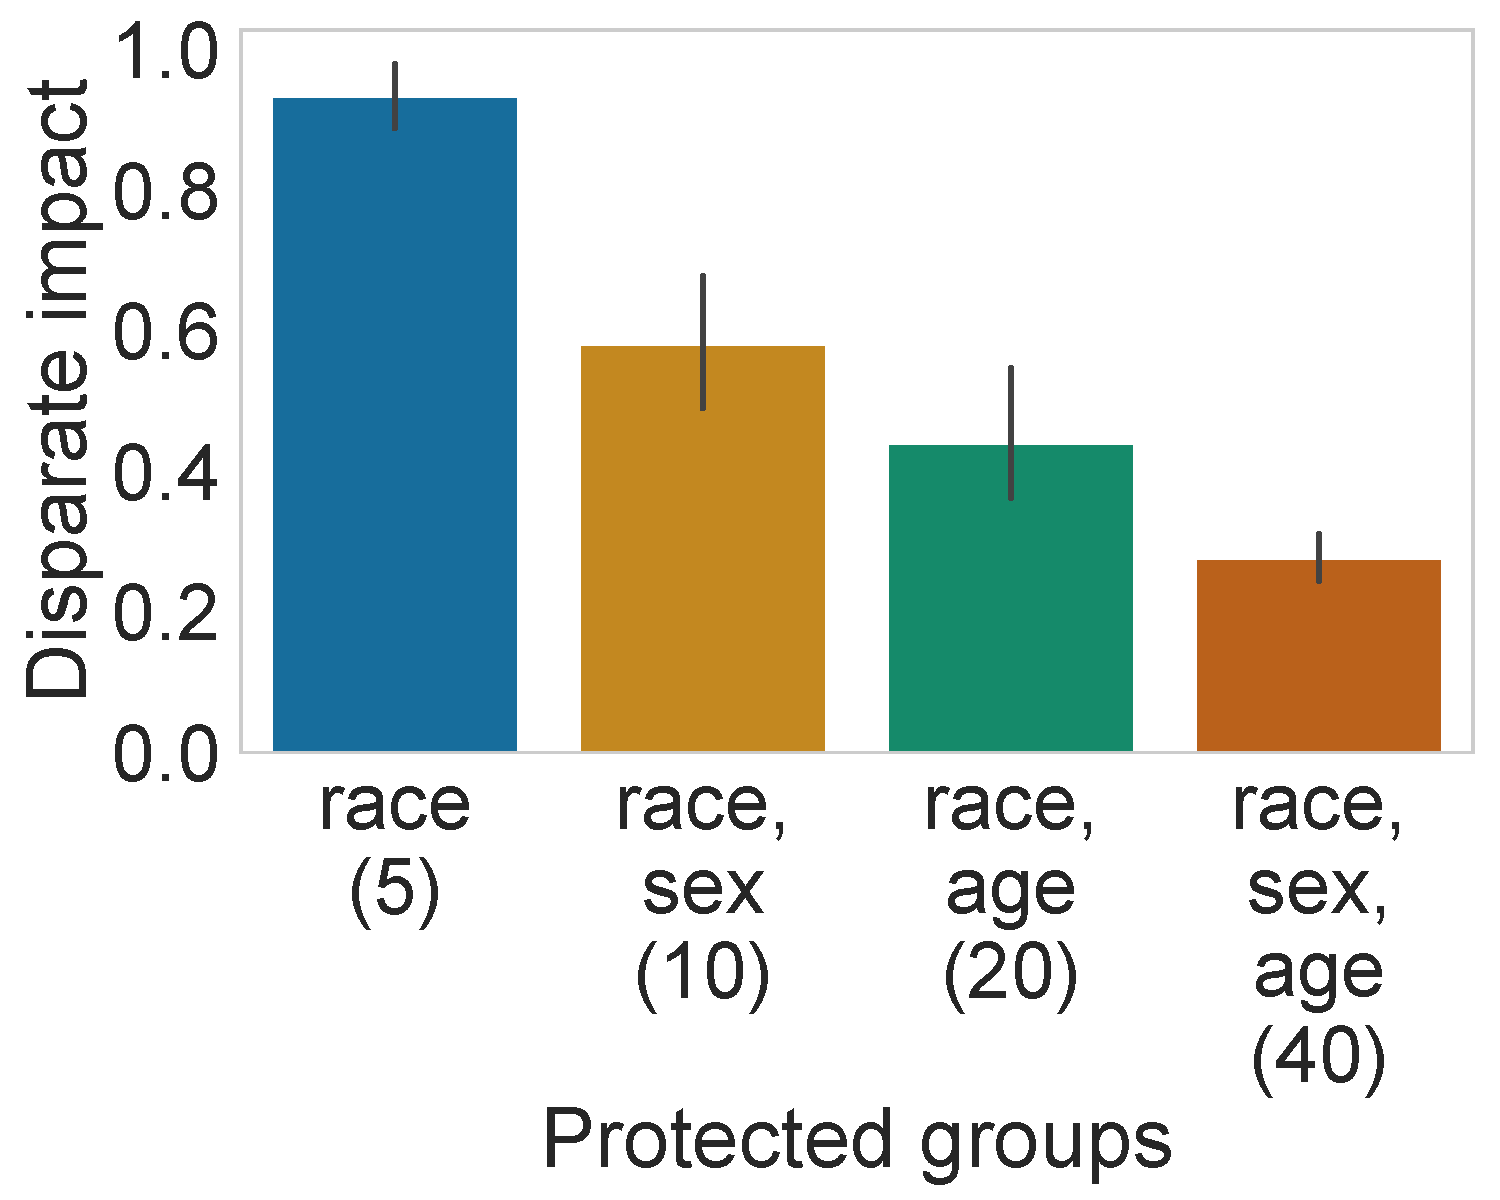
\includegraphics[scale=.2]{figures/fairness/justicia/sensitive_attribute_race_di_Adult_DT_RE.pdf}
	}
	\subfloat{
		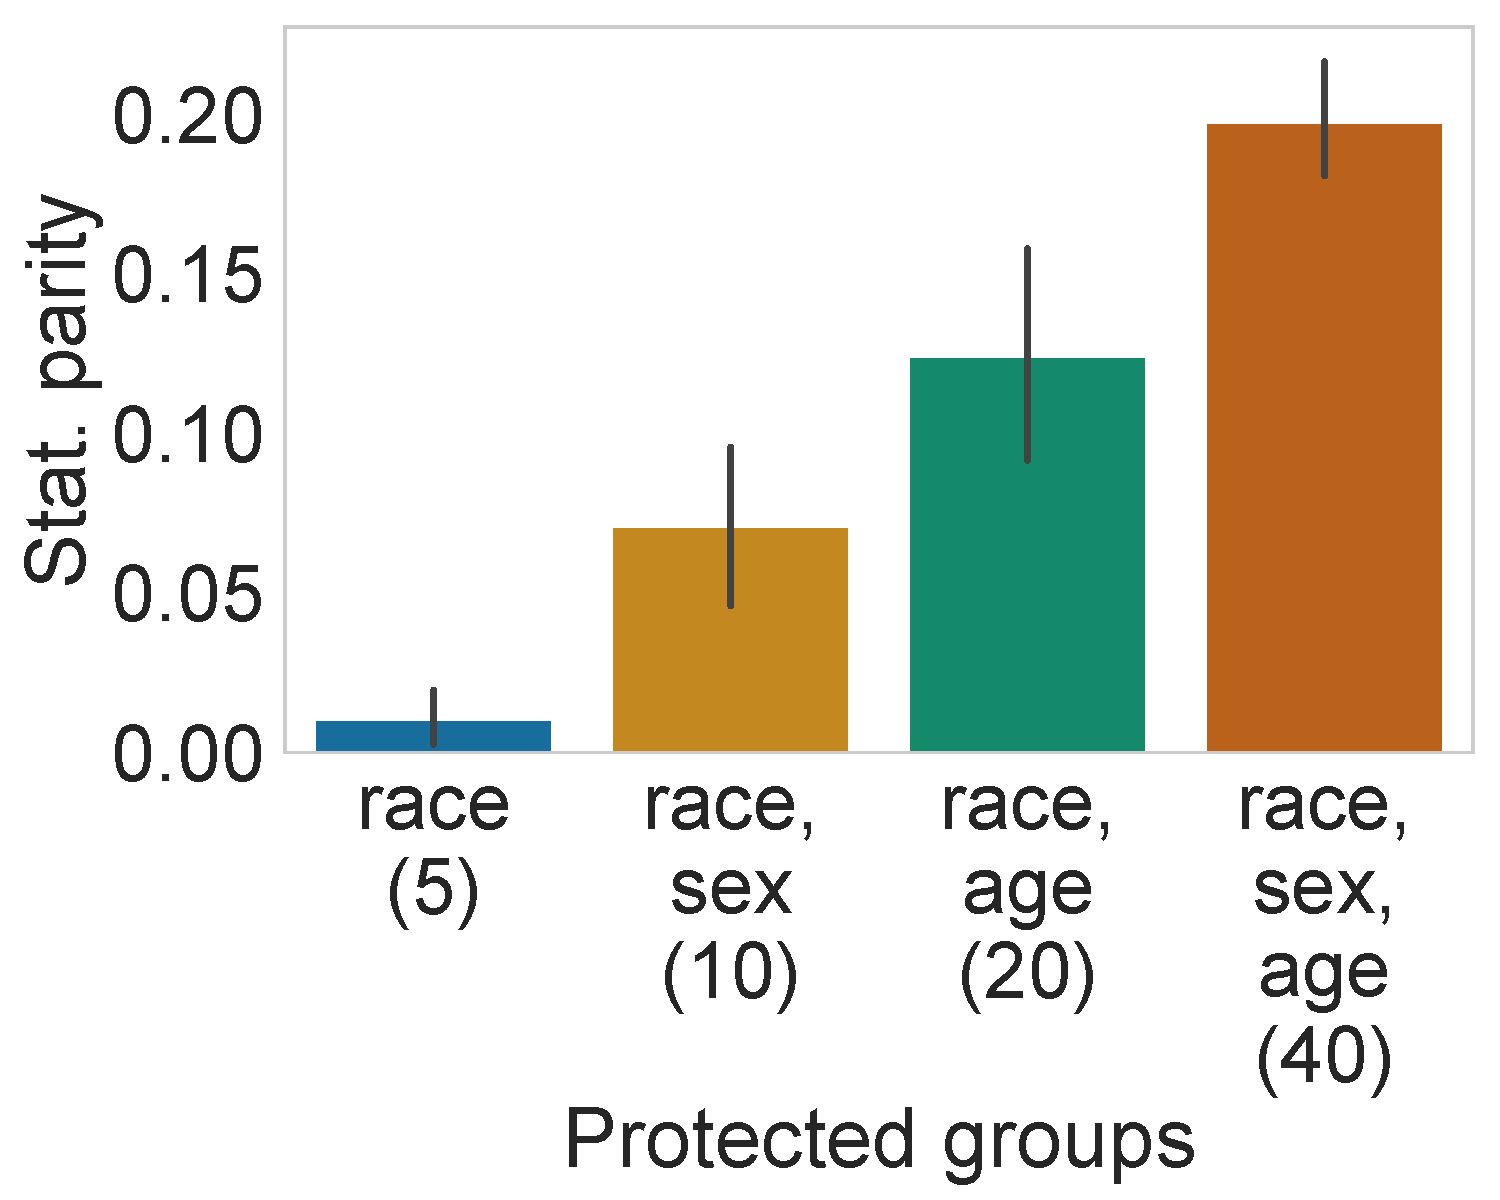
\includegraphics[scale=.2]{figures/fairness/justicia/sensitive_attribute_race_spd_Adult_DT_RE.pdf}
	}
	\caption{Fairness metrics measured by {\justicia} for different sensitive groups in the Adult dataset. The number within parenthesis in the xticks denotes total compound groups.}
	\label{fairness_justicia_fig:sensitive_groups}
\end{figure*}



\subsubsection{Verification: Detecting Compounded Discrimination in Protected Groups.}
We have tested {\justicia} for datasets consisting of multiple sensitive features and reported the results in Figure~\ref{fairness_justicia_fig:sensitive_groups}. {\justicia} operates on datasets with even 40 compound sensitive groups and can potentially scale more than that while the state-of-the-art fairness verifiers (e.g., FairSquare and VeriFair) consider a single sensitive feature.
Thus, {\justicia} removes an important limitation in practical fairness verification. 
Additionally, we observe in most datasets the disparate impact decreases and thus, discrimination increases as more compound sensitive groups are considered. For instance, when we increase the total  groups from $ 5 $ to $ 40 $ in the Adult dataset, disparate impact decreases from around $ 0.9 $ to $ 0.3 $, thereby detecting higher discrimination. Thus, {\justicia} detects that the marginalized individuals of a specific type (e.g., `race')  are even more discriminated and marginalized when they also belong to a marginalized group of another type (e.g., `sex').


\begin{sidewaystable}
	\caption[Fairness verification of fairness metrics and algorithms]{Verification of different fairness enhancing algorithms for multiple datasets and classifiers using {\justicia}. Numbers in bold refer to fairness improvement  compared against the unprocessed (orig.) dataset. RW and OP refer to reweighing and optimized-preprocessing algorithm respectively. }\label{fairness_justicia_tab:fair_algo_verification}
	\footnotesize       
    \centering
%        \setlength{\tabcolsep}{.3em}
            \begin{tabular}{ll
            				ccc
            				ccc
%            				ccc
%            				ccc
            				ccc
            				ccc}
                \toprule
                \multirow{3}{*}{Classifier}& Dataset $ \rightarrow $   & 
                \multicolumn{6}{c}{Adult} &
%                \multicolumn{6}{c}{German} &
                \multicolumn{6}{c}{COMPAS} \\ 
                \cmidrule(lr){3-8}
                \cmidrule(lr){9-14}
%                \cmidrule(lr){15-20}
                & Sensitive  $ \rightarrow $ & 
                \multicolumn{3}{c}{Race}   & \multicolumn{3}{c}{Sex}  &
%                \multicolumn{3}{c}{Age}   & \multicolumn{3}{c}{Sex}  &
                \multicolumn{3}{c}{Race}   & \multicolumn{3}{c}{Sex}
                \\ 
                \cmidrule(lr){3-5}
                \cmidrule(lr){6-8}
                \cmidrule(lr){9-11}
                \cmidrule(lr){12-14}
%                \cmidrule(lr){15-17}
%                \cmidrule(lr){18-20}

                 & Algorithm  $ \rightarrow $ &  
                orig. & RW & OP & 
                orig. & RW & OP &
%                orig. & RW & OP &
%                orig. & RW & OP &
                orig. & RW & OP &
                orig. & RW & OP \\ 
                \midrule
          
              
              
              \multirow{3}{*}{\shortstack{Logistic \\ regression}}
              & Disparte impact&  $ 0.23 $ &  $ \mathbf{0.85} $ &  $ \mathbf{0.59} $ &  $ 0.03 $ &  $ \mathbf{0.61} $ &  $ \mathbf{0.62} $ &  $ 0.34 $ &  $ \mathbf{0.36} $ &  $ \mathbf{0.47} $ &  $ 0.48 $ &  $ \mathbf{0.80} $ &  $ \mathbf{0.74} $  \\
              & Statistical parity&  $ 0.09 $ &  $ \mathbf{0.01} $ &  $ \mathbf{0.05} $ &  $ 0.16 $ &  $ \mathbf{0.04} $ &  $ \mathbf{0.03} $ &  $ 0.39 $ &  $ \mathbf{0.33} $ &  $ \mathbf{0.21} $ &  $ 0.23 $ &  $ \mathbf{0.09} $ &  $ \mathbf{0.10} $  \\
              & Equalized odds&  $ 0.13 $ &  $ \mathbf{0.03} $ &  $ \mathbf{0.10} $ &  $ 0.30 $ &  $ \mathbf{0.02} $ &  $ \mathbf{0.06} $ &  $ 0.38 $ &  $ \mathbf{0.33} $ &  $ \mathbf{0.18} $ &  $ 0.17 $ &  $ 0.19 $ &  $ \mathbf{0.07} $  \\
              \midrule
              \multirow{3}{*}{\shortstack{Decision \\ tree}}
              & Disparte impact&  $ 0.82 $ &  $ 0.60 $ &  $ 0.67 $ &  $ 0.00 $ &  $ \mathbf{0.73} $ &  $ \mathbf{0.95} $ &  $ 0.61 $ &  $ 0.58 $ &  $ 0.57 $ &  $ 0.94 $ &  $ 0.78 $ &  $ 0.63 $  \\
              & Statistical parity&  $ 0.02 $ &  $ 0.05 $ &  $ 0.04 $ &  $ 0.14 $ &  $ \mathbf{0.05} $ &  $ \mathbf{0.01} $ &  $ 0.18 $ &  $ \mathbf{0.17} $ &  $ \mathbf{0.17} $ &  $ 0.02 $ &  $ 0.09 $ &  $ 0.18 $  \\
              & Equalized odds&  $ 0.07 $ &  $ \mathbf{0.05} $ &  $ \mathbf{0.03} $ &  $ 0.47 $ &  $ \mathbf{0.03} $ &  $ \mathbf{0.04} $ &  $ 0.17 $ &  $ \mathbf{0.16} $ &  $ \mathbf{0.16} $ &  $ 0.07 $ &  $ \mathbf{0.05} $ &  $ 0.16 $  \\
              
              
              
              
              
               
               
                \bottomrule
    \end{tabular}

\end{sidewaystable}



\subsubsection{Verification: Fairness of Algorithms on Datasets.}
We have experimented with two fairness-enhancing algorithms: the reweighing (RW) algorithm and the optimized-preprocessing (OP) algorithm.
Both of them pre-process to remove statistical bias from the dataset. 
We study the effectiveness of these algorithms using {\justicia} on three datasets each with two different sensitive features.  
In Table~\ref{fairness_justicia_tab:fair_algo_verification}, we report different fairness metrics on logistic regression and decision tree. We observe that {\justicia} verifies fairness improvement as the bias mitigating algorithms are applied.  For example, for the Adult dataset with `race' as the sensitive feature, disparate impact increases from $ 0.23 $ to $ 0.85 $ for applying the reweighing algorithm on logistic regression classifier. In addition, statistical parity decreases from $ 0.09 $ to $ 0.01 $, and equalized odds decreases from $ 0.13 $ to $ 0.03 $, thereby showing the effectiveness of reweighing algorithm in all three fairness metrics. 
{\justicia} also finds instances where the fairness algorithms fail, specially when considering the decision tree classifier. 
Thus, {\justicia} enables verification of different fairness enhancing algorithms in literature.

\subsubsection{Robustness: Stability to Sample Size.} 
We have compared the robustness of {\justicia} with AIF360 by varying the sample-size and reporting the standard deviation of different fairness metrics. 
In Figure~\ref{fairness_justicia_fig:sample-size}, AIF360 shows higher standard deviation for lower sample-size and the value decreases as  the sample-size increases. 
In contrast, {\justicia} shows significantly lower ($\sim10\times$ to $100\times$) standard deviation for different sample-sizes. 
The reason is that AIF360 empirically measures on a fixed test dataset whereas {\justicia} provides estimates over the data generating distribution.
Thus, {\justicia} is more robust than the sample-based verifier AIF360.

\begin{figure*}
	\centering
	\subfloat{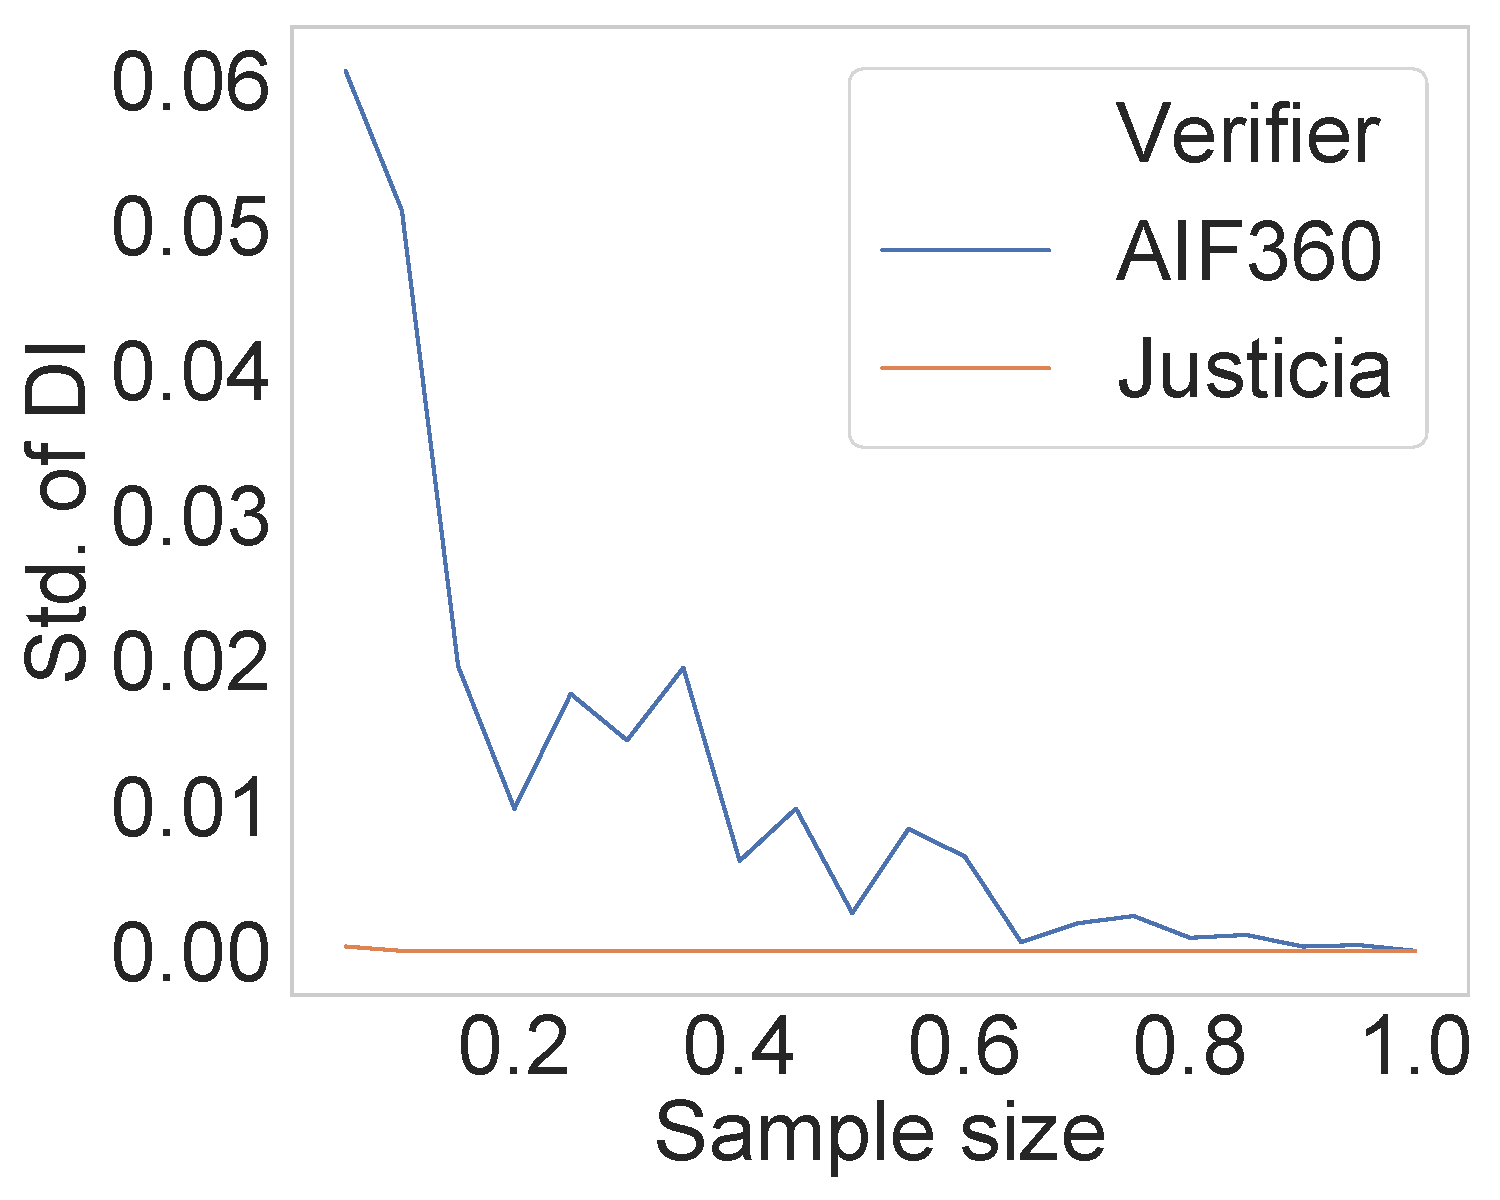
\includegraphics[scale=.2]{figures/fairness/justicia/sampling_DI_after_Adult_rw_LR_race.pdf}}
	\subfloat{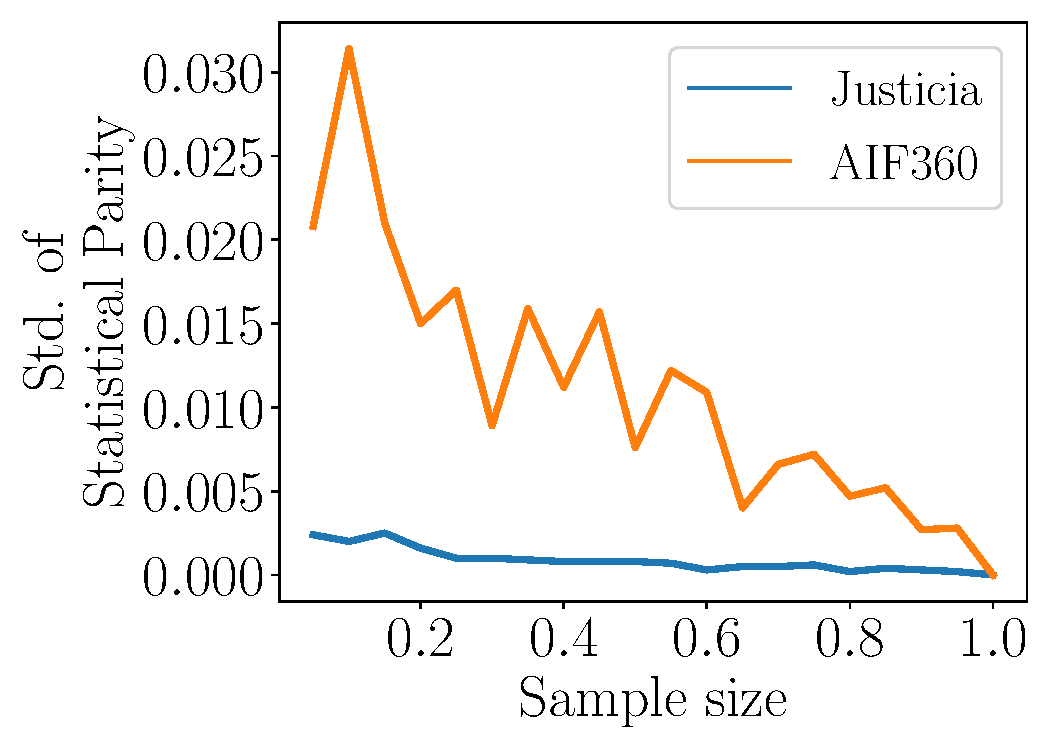
\includegraphics[scale=.2]{figures/fairness/justicia/sampling_SPD_after_Adult_rw_LR_race.pdf}}		\caption{Standard deviation in estimation of disparate impact (DI) and stat. parity (SP)  for different sample sizes. {\justicia} is more robust with variation of sample size than  AIF360. }
	\label{fairness_justicia_fig:sample-size}
\end{figure*}



\begin{figure}[t!]
	\begin{center}
		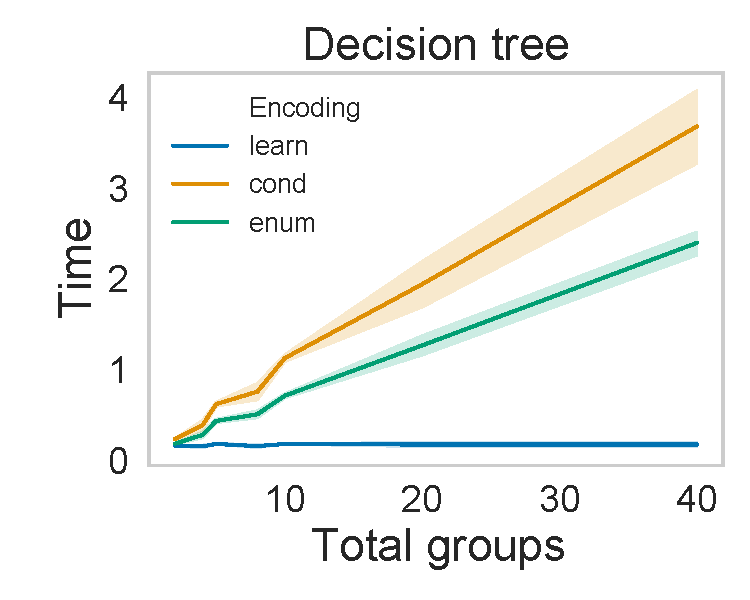
\includegraphics[scale=.4]{figures/fairness/justicia/encoding_runtime_Adult_DT.pdf}
		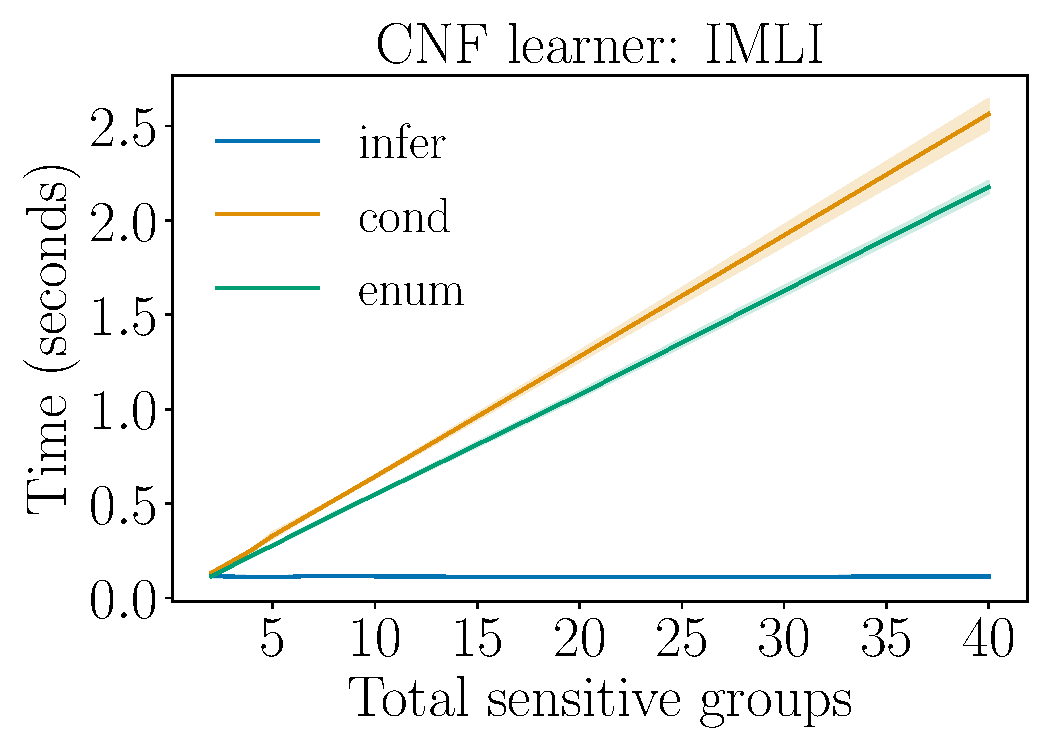
\includegraphics[scale=.4]{figures/fairness/justicia/encoding_runtime_Adult_IMLI.pdf}
		\hfill
		\caption{Runtime comparison of different encodings while varying total sensitive groups in the Adult dataset. \red{Label `learn' to be `infer'???}}
		\label{fairness_justicia_fig:runtime_diff_encodings}
	\end{center}
\end{figure}



\subsubsection{Comparative Evaluation of Different Encodings.}
While both {\justiciaenum} and {\justicialearn}  have the same output according to Lemma~\ref{fairness_justicia_lm:equivalence},  {\justicialearn} encoding  improves exponentially  in runtime  than {\justiciaenum} encoding on both decision tree and Boolean CNF classifiers as we vary the total compound groups in Figure~\ref{fairness_justicia_fig:runtime_diff_encodings}. {\justiciacond} (conditional probabilities w.r.t. sensitive groups) also has an exponential trend in runtime similar to {\justiciaenum}.  This analysis justifies that the na\"ive enumeration-based approach cannot verify large-scale fairness problems containing multiple sensitive features, and {\justicialearn} is a more efficient approach for practical use.

%The runtime efficiency of {\justicialearn} posits it as a more scalable and practical approach to verify fairness than {\justiciaenum}.
%\red{Justify the use of }.









				\section{Discussion and Future Work}
Though formal verification of different fairness metrics of an ML algorithm for different datasets is an important question, existing verifiers are not scalable, accurate, and extendable to non-Boolean sensitive features. We propose a stochastic SAT-based approach, {\justicia}, that formally verifies multiple group and causal fairness metrics for different classifiers and distributions for compound sensitive groups.
Experimental evaluations demonstrate that {\justicia} achieves \textit{higher accuracy} and \textit{scalability} in comparison to the state-of-the-art verifiers, FairSquare and VeriFair, while yielding \textit{higher robustness} than the sample-based tools, such as AIF360.

\red{Our work opens up several new directions of research. One direction is to develop SSAT models and verifiers for popular classifiers like Deep networks and SVMs. Other direction is to develop SSAT solvers that can accommodate continuous variables and conditional probabilities by design.}
%Of particular interest is the highlighted need for design of efficient SSAT solvers given that SSAT can be viewed as a natural target problem in the context of development of formal verification techniques for fairness.

%In this paper, we focus on formal verification of whether a given model satisfies a given fairness criterion. To this end, we proposed a stochastic SAT-based approach, {\justicia}, that formally verifies independence and separation metrics of fairness for different classifiers and distributions. We demonstrates that {\justicia} achieves higher accuracy and scalability in comparison to the prior state of the art approaches while achieving higher robustness in comparison to purely dataset based approaches such as AIF360. Our work opens up several directions of new research. Of particular interest is the highlighted need for design of efficient SSAT solvers given that SSAT can be viewed as a natural target problem in the context of development of formal verification techniques for fairness. 
				
				
%		FVGM
		\chapter{Algorithmic Fairness Verification with Graphical Models}
				\section{abstract}
In recent years, machine learning (ML) algorithms have been deployed in safety-critical and high-stake decision-making, where the \textit{fairness} of algorithms is of paramount importance. Fairness in ML  centers on detecting bias towards certain demographic populations induced by an ML classifier and proposes algorithmic solutions to mitigate the bias with respect to different fairness definitions.  To this end, several \textit{fairness verifiers} have been proposed that compute the bias in the prediction of an ML classifier\textemdash essentially beyond a finite dataset\textemdash given the probability distribution of input features. In the context of verifying \textit{linear classifiers}, existing fairness verifiers are limited by \emph{accuracy} due to imprecise modeling of correlations among features and \emph{scalability} due to restrictive formulations of the classifiers as SSAT/SMT formulas or by sampling. 

In this paper, we propose an efficient fairness verifier, called \fvgm, that encodes the correlations among features as a Bayesian network. In contrast to existing verifiers, \fvgm~proposes a \textit{stochastic subset-sum} based approach for verifying linear classifiers. Experimentally, we show that  \fvgm~leads to an \textit{accurate} and \textit{scalable} assessment for more diverse families of fairness-enhancing algorithms, fairness attacks, and group/causal fairness metrics than the state-of-the-art. We also demonstrate that {\fvgm} facilitates the computation of fairness influence functions as a stepping stone to detect the source of bias induced by subsets of features.



%that encodes the correlations among features as a Bayesian network and \red{enables disentangled measurement of bias induced by the data and the classifier}.






				%\section{Introduction}

\label{chapter:fvgm}
	The significant improvement of machine learning over the decades has led to a host of applications of machine learning in  high-stake decision-making such as college admission~\cite{martinez2021using}, hiring of employees~\cite{ajunwa2016hiring}, and recidivism prediction~\cite{tollenaar2013method,dressel2018accuracy}. Machine learning algorithms often have an accuracy-centric learning objective, which may cause them to be biased towards certain part of the dataset belonging to a certain economically or socially sensitive groups~\cite{landy1978correlates,zliobaite2015relation,berk2019accuracy}.
%	Fairness in Machine Learning (ML) has gained a significant focus  in recent years as ML algorithms are deployed in high-stake decision-making, such as college admission, hiring of employees, and recidivism prediction. Thus, if the ML algorithm is biased towards certain part of the dataset belonging to certain economically or socially sensitive groups, it can cause adverse effects in real-life.
	 The following example illustrates a plausible case of unfairness of machine learning. 
	\begin{example}\label{fvgm_example:intro}
		\normalfont
		Following Example~\ref{fairness_justicia_example:intro}, let us consider a machine learning classification where the classifier decides the eligibility of an individual for health insurance given their income and fitness (Figure~\ref{fvgm_fig:example1}). Here, the sensitive feature `age' ($ A $) follows a Bernoulli distribution, and income ($ I $) and fitness ($ F $) follow Gaussian distributions. We generate 1000 samples from these distributions and use them to train a Support Vector Machine (SVM) classifier. The decision boundary of this classifier is $9.37I + 9.75F - 0.34A \ge 9.4$, where $A = 1$ denotes the sensitive group `age $ \ge $ 40'. This classifier selects an individual above and below $40$ years of age with probabilities $0.24$ and $0.86$, respectively. This illustrates a disparate treatment of individuals of two age groups by the SVM classifier. 
	\end{example}
%	The above example illustrates that even in simple scenarios, ML-based solutions can lead to disparate treatment. Motivated by studies indicating that such scenarios are rather not uncommon, there is a thrust in the research on the improvement of fairness in ML by proposing different notions of fairness definitions and fairness algorithms~\cite{hardt2016equality,kusner2017counterfactual,mehrabi2019survey}. 

%KSM: Make the two plots side by side
\begin{figure}[h!]
	\begin{center}
		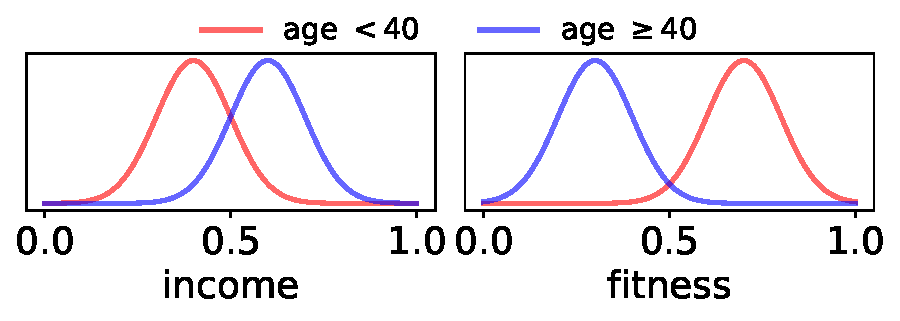
\includegraphics[scale = 0.5]{figures/fairness/fvgm/sanity_probability}
	\end{center}
	\caption[Illustrative distribution of features]{Age-dependent distributions of income and fitness in Example~\ref{fvgm_example:intro}.}\label{fvgm_fig:example1}
\end{figure}


	In order to identify and mitigate the bias of classifiers, different fairness definitions and fairness algorithms have been proposed~\cite{hardt2016equality,kusner2017counterfactual,mehrabi2019survey}.	In this chapter, we focus on two families of fairness definitions: \textit{group} and \textit{causal} fairness. Group fairness metrics, such as disparate impact and equalized odds constrain the probability of the positive prediction of the classifier to be (almost) equal among different sensitive groups~\cite{dwork2012fairness,feldman2015certifying}.	On the other hand, causal fairness metrics assess the difference in positive predictions  if every feature in the causal relation  remains identical except the sensitive feature~\cite{nabi2018fair,zhang2018fairness}. The early works on \textit{fairness verification} focused on measuring fairness metrics of a classifier for a given dataset~\cite{aif360-oct-2018}. Naturally, such techniques were limited in enhancing confidence of users for wide deployment. Consequently, recent verifiers seek to achieve verification beyond  finite dataset and in turn focus on the  probability distribution of features~\cite{albarghouthi2017fairsquare, bastani2019probabilistic, ghosh2020justicia}.  More specifically, the input to the verifier is a classifier and  the probability distribution of features, and the output is an estimate of fairness metrics that the classifier obtains given the distribution. For Example~\ref{fvgm_example:intro}, a fairness verifier takes the SVM classifier and the distribution of features $ I, F, A $ as an input and outputs the probability of positive prediction of the classifier for  different sensitive groups. 
	
%	\red{Despite extensive efforts over the past few years, the scalability and accuracy of fairness verifiers remains a major challenge. In particular, the existing techniques fail to scale beyond {\em toy} examples. In this work, we seek to remedy the situation. As a first step, we focus on  \textit{linear classifiers}, which has attracted a significant attention from researchers in the context of fair algorithms~\cite{pleiss2017fairness,zafar2017fairness,dressel2018accuracy, john2020verifying}. At this point, it is worth highlighting that our empirical evaluation demonstrates that the existing techniques fail to scale beyond small examples or provide highly inaccurate estimates for comparatively {\em small} linear classifiers. }
 	
	
	In order to solve the fairness-verification problem, existing works have proposed two principled approaches.	Firstly, \cite{ghosh2020justicia} and \cite{albarghouthi2017fairsquare} propose formal methods that reduce the problem into a solution of an SSAT or an SMT~ formula respectively.	Secondly, \cite{bastani2019probabilistic} propose a sampling approach that relies on extensively enumerating the conditional probabilities of prediction given different sensitive features and thus, incurs high computational cost. Additionally, existing works assume feature independence of non-sensitive features and consider correlated features within a limited scope, such as conditional probabilities of non-sensitive features w.r.t. sensitive features and ignore correlations among non-sensitive features. As a result, the \textit{scalability} and \textit{accuracy} of existing  verifiers remains a major challenge.
	
	In this work, we seek to remedy the aforementioned situation. As a first step, we focus on  \textit{linear classifiers}, which has attracted significant attention from researchers in the context of fair algorithms~\cite{pleiss2017fairness,zafar2017fairness,dressel2018accuracy, john2020verifying}. At this point, it is worth highlighting that our empirical evaluation demonstrates that the existing techniques fail to scale beyond small examples or provide highly inaccurate estimates for comparatively {\em small} linear classifiers. 
	
%	In this paper, we argue that the above solution is not practical in verifying linear classifiers for two reasons: (i) the encoding of a linear classifier into an SSAT or an SMT formula or using a sampling approach suffer from scalability and (ii) ignoring correlations among all features results in an inaccurate estimate of fairness metrics. 	
	
	
%	Given multiple fairness definitions, fairness algorithms either \textit{preprocess} the training data~\cite{calmon2017optimized,kamiran2012data,zemel2013learning}, \textit{in-process} the classifier during training~\cite{zhang2018mitigating}, or \textit{post-process} the prediction of the trained classifiers~\cite{hardt2016equality,kamiran2012decision} to improve fairness. In contrast, fairness-attack algorithms try to manipulate the data or the classifier to worsen its fairness~\cite{solans2020poisoning}. 
	

	
%	\red{Among different ML classifiers, researcher This observation motivates us in asking the following research question: \textit{Can we design an efficient fairness verification framework for linear classifiers that can verify different fairness definitions and algorithms accurately?} 

	
	
%	
%	Considering the surge of research in ML fairness based on linear classifiers, we focus on designing a fairness verifier particularly tailored for linear classifiers. We further show novel applications of the verifier in practical fairness tasks, such as detecting fairness attacks and computing the source of unfairness in the level of input features.
%	
	

	
	
	\paragraph{Our Contributions.} The contributions of this chapter are summarized below.
	
	\begin{itemize}
		\item \textit{Framework:} In this chapter, we propose a fairness verification framework, namely {\fvgm} (\textbf{F}airness \textbf{V}erification with \textbf{G}raphical \textbf{M}odels), for accurately and efficiently verifying linear classifiers.
		\item \textit{Scalability:} {\fvgm} proposes a novel \textit{stochastic subset-sum} encoding for linear classifiers with an efficient pseudo-polynomial solution using dynamic programming.
		\item \textit{Accuracy:} To address feature-correlations, {\fvgm} considers a graphical model, particularly a Bayesian Network that represents conditional dependence (and independence) among features in the form of a Directed Acyclic Graph (DAG). 
		\item \textit{Experimental Results:}	Experimentally,  {\fvgm} is more accurate and scalable than existing fairness verifiers; {\fvgm} can verify group and causal fairness metrics for multiple fairness algorithms.
		\item \textit{Applications:} We also demonstrate two novel applications of {\fvgm} as a fairness verifier: (a) detecting fairness attacks, and (b) computing Fairness Influence Functions (FIF) of features as a mean of identifying (un)fairness contribution of a subset of features. 
	\end{itemize}
 



				
	\section{Background}
	In this section, we define different fairness metrics proposed for classification. Following that, we state basics of stochastic subset sum and Bayesian networks that are the main components of our methodology.
	
	\textbf{Fairness in ML.}
	We consider\footnote{{We represent sets/vectors by bold letters, and the corresponding distributions by calligraphic letters. We express random variables in uppercase, and an assignment of a random variable in lowercase.}} a dataset $ \mathbf{D} $ as a collection of triples $ (\nonsensitive, \sensitive, Y) $ generated from an underlying distribution $\mathcal{D}$. $ \nonsensitive \triangleq \{X_1, \dots, X_{m_1}\} $ are non-sensitive features whereas $ \sensitive \triangleq \{A_1, \dots, A_{m_2}\} $ are categorical sensitive features.  $Y \in \{0,1\}$ is the binary label (or class) of $(\nonsensitive,\sensitive)$. Each non-sensitive feature $ X_i$ is sampled from a continuous probability distribution {$ \mathcal{X}_i $}, and each sensitive feature $ A_j \in \{0, \dots, N_j\}  $ is sampled from a discrete probability distribution {$ \mathcal{A}_j $}. 
%	\red{Therefore, the distribution $\mathcal{D}$ is the joint distribution on $(\nonsensitive,\sensitive)$, where  $\mathcal{X}_i$ and $\mathcal{A}_i$ are the marginal distributions.} 
	%Therefore, $ \mathcal{D} = \prod_{i=1}^{m} \mathcal{X}_i \prod_{j=1}^{n} \mathcal{A}_j $ denotes the product distribution of sensitive and non-sensitive features and thus considered the underlying distribution for the dataset $ D $.  Additionally, $ Y \in \{0,1\} $ denotes the binary class label of $ (\nonsensitive, \sensitive) $. Let $ \alg : (\nonsensitive, \sensitive) \rightarrow \hat{Y} $  be a binary classier trained on $ D $, where $ \hat{Y} \in \{0,1\} $ is the predicted class. The positive predictive value (PPV) of $ \alg $, denoted as $ \Pr[\hat{Y} = 1] $, is the probability of positive outcome.
 	We use $ (\mathbf{x}, \mathbf{a}) $ to denote the feature-values of  $ (\nonsensitive, \sensitive) $.  For sensitive features, a valuation vector $ \mathbf{a} = [a_1, .., a_{m_2}] $ is called a \textit{compound sensitive group}. For example, consider $ \sensitive = $ \{race, sex\} where race $ \in $ \{Asian, Color, White\} and sex $ \in $ \{female, male\}. Thus $ \mathbf{a} = $ [Asian, female]  is a compound sensitive group. 
 	We represent a binary classifier trained on the dataset $\mathbf{D}$ as $\alg: (\nonsensitive, \sensitive) \rightarrow \hat{Y} $. Here, $\hat{Y} \in \{0,1\}$ is the predicted class of $ (\nonsensitive, \sensitive) $.
 	
 	We now discuss different fairness metrics in the literature based on the prediction of a classifier~\cite{feldman2015certifying,hardt2016equality,nabi2018fair}.  	
 	In this paper, {\fvgm} verifies two families of fairness metrics: group fairness (first three in the following) and path-specific causal fairness.

 	\begin{enumerate}[leftmargin=*]
 		\itemsep0em 
 		\item \textit{Disparate impact} (DI): A classifier  satisfies $(1 - \epsilon)$-disparate impact if for $\epsilon \in [0,1] $,
 		$
 		\min_{\mathbf{a}} \Pr[\hat{Y} =1 | \mathbf{A} =  \mathbf{a}]  \ge (1 - \epsilon) \max_{\mathbf{a}'} \Pr[\hat{Y} =1 | \mathbf{A} =  \mathbf{a}'].
 		$
 		\item \textit{Statistical Parity} (SP): A classifier satisfies $\epsilon$-statistical parity if for $\epsilon \in [0,1] $, 
 		$
 		\max_{\mathbf{a}, \mathbf{a}'}|\Pr[\hat{Y} =1 | \mathbf{A} = \mathbf{a}] - \Pr [\hat{Y} = 1| \mathbf{A} = \mathbf{a}']| \le \epsilon.
 		$
 		\item \textit{Equalized Odds} (EO): 	A classifier satisfies $\epsilon$-equalized odds if for $\epsilon \in [0,1] $,
 		$ \max_{\mathbf{a}, \mathbf{a}'} |\Pr[\hat{Y} =1 |\mathbf{A}= \mathbf{a}, Y= 0  ] - \Pr [\hat{Y} = 1|\mathbf{A}= \mathbf{a}', Y = 0]| \le \epsilon, $ and $
 		\max_{\mathbf{a}, \mathbf{a}'}|\Pr[\hat{Y} =1 |\mathbf{A}= \mathbf{a}, Y= 1  ] - \Pr [\hat{Y} = 1|\mathbf{A}= \mathbf{a}', Y = 1]| \le \epsilon.
 		$
 		\item \textit{Path-specific Causal Fairness} (PCF): 
 		Let $ \mathbf{a}_{\max}  \triangleq \argmax_{ \mathbf{a}} \Pr[\hat{Y} =1 |\mathbf{A}=  \mathbf{a}] $. We consider mediator features $ \mediator \subseteq \nonsensitive $ sampled from the conditional distribution $ {\mathcal{Z}_{|\mathbf{A} = \mathbf{a}_{\max}}} $. This emulates the fact that mediator variables have the same sensitive features $ \mathbf{a}_{\max} $.  For $ \epsilon \in [0,1] $,  path-specific causal fairness is defined as 
 		$
 		\max_{\mathbf{a}, \mathbf{a}'} |\Pr[\hat{Y} = 1 | \sensitive =  \mathbf{a}, \mediator] - \Pr[\hat{Y} = 1 | \sensitive = \mathbf{a}', \mediator ]| \le \epsilon
 		$.
 	\end{enumerate}

 	  For all of the above metrics, lower value of $\epsilon$ indicates higher fairness demonstrated by the classifier $\mathcal{M}$. Following the observation of~\cite{ghosh2020justicia},  computing all of the aforementioned fairness metrics is equivalent to computing the maximum and minimum of the \textit{Positive Predictive Value} (PPV) of the classifier, denoted as $\Pr[\hat{Y}=1|\mathbf{A} =\mathbf{a}]$, for all compound sensitive groups $\mathbf{a}$ from $ \sensitive $. Thus, in Section~\ref{fairness_fvgm_sec:fvgm}, we focus on computing the maximum and minimum PPVs and then extend it to assess corresponding fairness metrics. We call the group for which PPV is maximum (minimum) as the \textit{most (least) favored group}.
 
% 	\textit{Disparate impact} (DI)~\cite{feldman2015certifying} measures the ratio of PPVs between the most favored group and least favored group, and prescribe it to be close to $1$. Formally, 
% 	Another popular relaxation of independence metrics  is \textit{statistical parity} (SP) that measures the difference of PPV among sensitive groups, and prescribe this to be near zero. Formally, an algorithm satisfies $\epsilon$-statistical parity if, for $\epsilon \in [0,1] $, 
% 	\[
% 	\max_{\mathbf{a}_i, \mathbf{a}_j \in A}|\Pr[\hat{Y} =1 | A = \mathbf{a}_i] - \Pr [\hat{Y} = 1| A = \mathbf{a}_j]| \le \epsilon.
% 	\] 	
% 	
% 	In the \textit{separation (or classification parity)} notion of fairness, the predicted label $\hat{Y}$ of a classifier $\alg$ is independent of the sensitive features $A$ given the actual class labels $Y$. In case of binary classifiers, a popular separation metric is \textit{equalized odds} (EO)~\cite{hardt2016equality} that computes the difference of false positive rates (FPR) and the difference of true positive rates (TPR) among all compound sensitive groups. 
% 	Lower value of equalized odds indicates better fairness.
% 	A classifier $\alg$ satisfies $\epsilon$-equalized odds if, for all compound sensitive groups $\mathbf{a}, \mathbf{a} \in A$,
% 	\begin{equation}
% 	\begin{split}
% 	|\Pr[\hat{Y} =1 | A = \mathbf{a}, Y= 0  ] - \Pr [\hat{Y} = 1| A = \mathbf{a}, Y = 0]| &\le \epsilon, \\ 
% 	|\Pr[\hat{Y} =1 | A = \mathbf{a}, Y= 1  ] - \Pr [\hat{Y} = 1| A = \mathbf{a}, Y = 1]| &\le \epsilon.\notag
% 	\end{split}
% 	\end{equation}
% 	
% 	Path-specific causal fairness (PCF) states that the outcome $ \hat{Y} $ should not depend directly on a sensitive feature, but may depend indirectly on the sensitive feature through other \textit{mediator} features[\cite{?}]. 
% 	
% 	
% 	
% 	\red{Need to clarify, group fairness and causal fairness?}
% 	
% 	
% 	\blue{It may be space consuming to discuss different fairness metrics, in which case we can mention that computing PPV is the core component of estimating different fairness metrics.}
% 

	\textbf{Stochastic Subset Sum Problem ({\stochastic}).} 
	Let $ \mathbf{B} \triangleq \{B_i\}_{i=1}^{|\mathbf{B}|}$ be a set of Boolean variables and $ w_i \in \mathbb{Z} $ be the weight of $ B_i $. Given a constraint of the form  $\sum_{i = 1}^ {|\mathbf{B}|} w_i B_i = \tau $, for a constant $ \tau \in \mathbb{Z} $, the subset-sum problem seeks to compute $\mathbf{b} \in \{0,1\}^{|\mathbf{B}|}$ such that the constraint evaluates to true when $\mathbf{B}$ is substituted with $\mathbf{b}$. Subset sum problem is known to be a $ \mathrm{NP} $-complete problem and well-studied in theoretical computer science~\cite{kleinberg2006algorithm}. The \textit{counting} version of the subset-sum problem counts all $ \mathbf{b} $'s for which the above constraint holds; and this problem belongs to the complexity class $ \mathrm{\#P} $. In this paper, we consider the counting problem for the constraint $\sum_{i = 1}^ {|\mathbf{B}|} w_i B_i \ge \tau $ where variables $ B_i $'s are stochastic. More precisely, we define a \textit{stochastic subset-sum} problem, namely {\stochastic}, that computes $ \Pr[\sum_{i = 1}^ {|\mathbf{B}|} w_iB_i \ge \tau] $.    Details of {\stochastic} are in Section~\ref{fairness_fvgm_sec:stochastic_sum_set_sum}.
	
	
		
	\textbf{Bayesian Network.}
	In general, a Probabilistic Graphical Model~\cite{koller2009probabilistic}, and specifically a \textit{Bayesian network}~\cite{pearl1985bayesian,chavira2008probabilistic}, encodes the dependencies and conditional independence between a set of random variables. In this paper, we leverage an access to a Bayesian network on $(\nonsensitive, \sensitive)$ that represents the joint distribution on them. 
	A Bayesian network is denoted by a pair $ (\graph, \theta)$, where $ \graph \triangleq (\mathbf{V}, \mathbf{E}) $ is a Directed Acyclic Graph (DAG), and $\theta$ is a set of parameters that encodes the conditional probabilities induced by the joint distribution under investigation. Each vertex $V_i \in \mathbf{V}$ corresponds to a random variable. Edges $ \mathbf{E} \in \mathbf{V} \times \mathbf{V} $ imply conditional dependencies among variables. For each variable $ V_i \in \mathbf{V} $, let $ \parent(V_i) \subseteq \mathbf{V} \setminus \{V_i\} $ denote the set of parents of $ V_i $. Given $\parent(V_i)$ and parameters $\theta$, $ V_i $ is independent of its other non-descendant variables in $\graph$. Thus, for the assignment $ v_i $ of $ V_i $ and $ \mathbf{u} $ of $ \parent(V_i) $, the aforementioned semantics of a Bayesian network encodes the joint distribution of $\mathbf{V}$ as:
	
	\begin{align}
	\Pr[V_1=v_1, \dots, V_{|\mathbf{V}|}=v_{|\mathbf{V}|}] = \prod_{i=1}^{|\mathbf{V}|} \Pr[V_i = v_i | \parent(V_i) = \mathbf{u}; \theta].
	\label{fairness_fvgm_eq:BN}
	\end{align}

	\iffalse	
	$ \factors $ contains a factor $ \factor $ representing a function over the  assignment or valuation of  $ \{V_i\} \cup \parent(V_i)  $. Let $ v $ and $ \mathbf{u} $ denote an assignment of $ V_i $ and $ \parent(V_i) $, respectively. 	Formally a factor $ \factor(V_i = v, \parent(V_i) = \mathbf{u}) \triangleq  \Pr[V_i = v | \parent(V_i) = \mathbf{u}] $ denotes the conditional probability of $ V_i = v $ given $ \parent(V_i) = \mathbf{u} $. Avoiding notation clutter, we drop $ v $ and $ \mathbf{u} $ and use $ \factor(V_i, \parent(V_i)) \triangleq  \Pr[V_i| \parent(V_i)] $, when it is clear from the context.
	\fi
	
				\section{Fairness Verification with Graphical Models}\label{fvgm_sec:fvgm}

In this section, we present {\fvgm}, a fairness verification framework for linear classifiers that accounts for correlated features represented as a graphical model. The core idea of verifying fairness of a classifier is to compute the probability of positive prediction of the classifier with respect to all compound sensitive groups. To this end, {\fvgm} solves a stochastic subset sum problem, {\stochastic}, that is equivalent to computing the probability of positive prediction of the classifier for the most and the least favored sensitive group\footnote{The most (resp.\ least) favored sensitive group obtains the maximum (resp.\ minimum) probability of positive prediction of the classifier.}. In this section, we first define {\stochastic} and present an efficient dynamic programming solution for {\stochastic}. We then extend {\stochastic} to consider correlated features as input. Finally, we conclude by discussing fairness verification based on the solution of {\stochastic}.


\paragraph{Problem Formulation.}	
Given a linear classifier $ \alg: (\nonsensitive, \sensitive) \rightarrow \widehat{Y} $ and a probability distribution $ \mathcal{D} $ of $ \nonsensitive \cup \sensitive $, our objective is to compute $ \max_{ \mathbf{a}} \Pr[\widehat{Y} =1 | \sensitive = \mathbf{a}] $ and $ \min_{ \mathbf{a}} \Pr[\widehat{Y} =1 | \sensitive = \mathbf{a}] $ with respect to $ \mathcal{D} $. In this study, we express a linear classifier $\mathcal{M}$ as 

\[	\widehat{Y} = \mathds{1}\Big[\sum_{i} W_{X_i}X_i + \sum_{j} W_{A_j}A_j \ge \tau\Big].\]

Here, $ W $ denotes the weight (or coefficients) of a feature, $ \tau $ denotes the bias or the offset parameter of the classifier, and $\mathds{1}$ is an indicator function. Hence, the prediction $ \widehat{Y} =1 $ if and only if the inner inequality holds.
Thus, computing the maximum (resp.\ minimum) probability of positive prediction is equivalent to finding out the assignment of $A_j$'s for which the probability of satisfying the inner inequality is highest (resp.\ lowest). We reduce this computation into an instance of {\stochastic}. To perform this reduction, we assume  weight $ W $ and bias $ \tau $ as integers, and features $\nonsensitive \cup \sensitive $ as Boolean. In Sec.~\ref{fvgm_sec:practical}, we relax these assumptions and extend to the practical settings. 

\subsection{Stochastic Subset Sum Problem}\label{fvgm_sec:stochastic_sum_set_sum}
Now, we formally describe the specification and semantics of {\stochastic}.
{\stochastic} operates on  a set of Boolean variables $ \mathbf{B} = \{B_i\}_{i=1}^{n} \in \{0,1\}^{n} $, where $ W_i \in \mathbb{Z} $ is the weight of $ B_i $, and $n \triangleq |\mathbf{B}|$. Given a constant threshold $ \tau \in \mathbb{Z} $, {\stochastic} computes the \textit{probability} of a subset of $ \mathbf{B} $ with sum of weights of non-zero variables to be at least $ \tau $. Formally,

\[S(\mathbf{B}, \tau) \triangleq \Pr\Big[\sum_{i} W_iB_i \ge \tau \Big].\]

Aligning with terminologies in stochastic satisfiability (SSAT)~\cite{littman2001stochastic}, we categorize the variables $ \mathbf{B} $ into two types: (i) \textit{chance variables} that are stochastic and have an associated probability of being assigned to $ 1 $ and (ii) \textit{choice variables} that we  optimize while computing $ S(\mathbf{B}, \tau) $.  To specify the category of variables, we consider a \textit{quantifier} $ Q_i \in \{\R^{p_i}, \exists, \forall\} $ for each $ B_i $. Elaborately, $ \R^{p} $ is a \textit{random quantifier} corresponding to a chance variable $ B \in \mathbf{B} $, where  $ p\triangleq \Pr[B = 1]$. In contrast, $ \exists $ is an \textit{existential quantifier} corresponding to a choice variable $ B $ such that a Boolean assignment of $ B $  \textit{maximizes}  $ S(\mathbf{B}, \tau) $. Finally, $ \forall $ is an \textit{universal quantifier} for a choice variable $ B $ that fixes an assignment to $ B $ that \textit{minimizes} $ S(\mathbf{B}, \tau) $. 
 
Now, we formally present the semantics of $ S(\mathbf{B}, \tau) $ provided that each variable $ B_i $ has weight $ W_i $ and quantifier $ Q_i $. Let  $ \mathbf{B}[2:n] \triangleq \{B_j\}_{j=2}^{n} $ be the subset of $\mathbf{B}$ without the first variable $ B_1 $. Then $ S(\mathbf{B}, \tau) $ is recursively defined as:


\begin{align}\label{fvgm_eq:semantics_recurse}
  S(\mathbf{B},\tau) =
 \begin{cases}
 \mathds{1}[ \tau \le 0 ], \; \text{if } \textbf{B} = \emptyset \\
 S(\mathbf{B}[2:n],\tau - \max\{W_1, 0\}), \; \text{if } Q_1 = \exists\\
 S(\mathbf{B}[2:n],\tau - \min\{W_1, 0\}), \; \text{if } Q_1 = \forall\\
 p_1\times S(\mathbf{B}[2:n],\tau - W_1) +\\ (1-p_1)\times S(\mathbf{B}[2:n],\tau),\; \text{if } Q_1 = \R^{p_1}
 \end{cases}
\end{align} 


%\begin{enumerate}
% 	\item $ S(\mathbf{B},\tau) = \mathds{1}[ \tau \le 0 ] $, if $ \textbf{B} = \emptyset $, %Here $ \mathds{1}[\text{true}] = 1 $ and $ \mathds{1}[\text{false}] = 0 $,
% 	\item $ S(\mathbf{B},\tau) = S(\mathbf{B}_{-1},\tau - \max\{W_1, 0\}) $, if $ Q_1 =  \exists $,
% 	\item $ S(\mathbf{B},\tau) = S(\mathbf{B}_{-1},\tau - \min\{W_1, 0\}) $, if $ Q_1 =  \forall $,
% 	\item $ S(\mathbf{B},\tau) = p_1S(\mathbf{B}_{-1},\tau - W_1) + (1-p_1) S(\mathbf{B}_{-1},\tau) $, if $ Q_1 = \R^{p_1}  $.
%\end{enumerate} 
%KSM: Don't use semantic 1, semantic 2, -- very confusing

Observe that when $ \textbf{B} $ is empty, $S$ is computed as $ 1 $ if $ \tau \le 0 $, and  $ S = 0 $ otherwise. For  existential and universal quantifiers, we compute $ S $ based on the weight. Specifically, if $ Q_1 = \exists $, we decrement the threshold $ \tau $ by the maximum between $ W_1 $ and $ 0 $. For example, if $ W_1 > 0 $, $ B_1 $ is assigned $ 1 $, and assigned $ 0 $ otherwise. Therefore, by solving for an existential variable, we  maximize $ S $. In contrast, when if $ Q_1 = \forall $, we fix an assignment of $ B_1 $ that minimizes $ S $ by choosing between the minimum of $ W_1 $ and $ 0 $. Finally, for random quantifiers, we decompose the computation of $S$ into two sub-problems: one sub-problem where $ B_1 = 1 $ and the updated threshold becomes $ \tau - W_1 $ and another sub-problem where $ B_1 = 0 $ and the updated threshold remains the same. Herein, we compute $ S $ as the expected output of both sub-problems.

%KSM: Lemma is a very strong term for such a straightforward observation
\begin{remark}
	\label{fvgm_lm:property_s3p}
	$ S(\mathbf{B},\tau) $ does not depend on the order of $ \mathbf{B} $.
\end{remark}

\paragraph{Computing Minimum and Maximum probability of positive prediction of Linear Classifiers Using  {\stochastic}.} For computing $ \max_{ \mathbf{a}} \Pr[\widehat{Y} =1 | \sensitive = \mathbf{a}] $ of a linear classifier, we set existential quantifiers $ \exists $ to sensitive features $ A_j $, randomized quantifiers $ \R $ to non-sensitive features $ X_i $ and construct a set $ \mathbf{B} = \sensitive \cup \nonsensitive $.  The coefficients $ W_{A_j} $ and $ W_{X_i} $ of the classifier become weights of $ \mathbf{B} $. Also, we get $n=m_1 +m_2$. For non-sensitive variables $ X_i $, which are chance variables, we derive their marginal probability $ p_i = \Pr[X_i = 1] $ from the distribution $ \mathcal{D} $.  According to semantic of {\stochastic}, setting $ \exists $ quantifiers on $ \sensitive $ computes the maximum value of $ S(\mathbf{B}, \tau) $ that equalizes the maximum probability of positive prediction of the classifier. In this case, the \textit{inferred} assignment of $ \sensitive $ implies the most favored group $ \mathbf{a}_{{\max}} =  \argmax_{ \mathbf{a}} \Pr[\widehat{Y} =1 | \sensitive = \mathbf{a}] $. In contrast, to compute the minimum probability of positive prediction, we instead assign each variable  $ A_j $ a universal  quantifier  while keeping random quantifiers over $ X_i $, and infer the least favored group $ \mathbf{a}_{{\min}} =  \argmin_{ \mathbf{a}} \Pr[\widehat{Y} =1 | \sensitive = \mathbf{a}] $.

\iffalse
\red{The decision version of computing the maximum (minimum) \red{\red{probability of positive prediction}} is to decide whether there is an assignment of \textit{sensitive} or \textit{choice variables}, for which the \textit{non-sensitive} or \textit{chance variables} yield a \red{\red{probability of positive prediction}} greater or less than $\alpha \in [0,1]$. Now, we formally state the hardness of verifying linear classifiers followed by an efficient dynamic programming solution.
\begin{lemma}
	\label{fvgm_lm:hardness}
	The decision version of the fairness verification problem for linear classifiers is in $\mathrm{NP^{PP}}$.
\end{lemma}}
\fi

 
 
 \subsection{A Dynamic Programming Solution}
 \label{fvgm_sec:dp_formulation}
 %\dbcomment{Use $ \mathsf{dp}(i, \tau) $ given $ B $}

We propose a dynamic programming approach~\cite{pisinger1999linear,woeginger1992equal} to solve {\stochastic} as the problem has overlapping sub-problem properties. 
For example, $S(\mathbf{B}, \tau)$ can be solved by solving $S(\mathbf{B}[2:n], \tau')$, where the updated threshold $\tau'$, called the \textit{residual threshold}, depends on the original threshold $\tau$ and the assignment of $B_1$ as shown in Eq.~\eqref{fvgm_eq:semantics_recurse}.
%\red{For example, the residual threshold $ \tau $ can be equal for a fixed subset of $ \mathbf{B} $, say $ \mathbf{B}[i:n] \triangleq \{B_j\}_{j=i}^{n} $, derived from different assignments of $ B_1, \dots, B_{i-1} $.} 
Building on this observation, we propose the recursion and terminating condition leading to our dynamic programming algorithm. 

\textit{Recursion.} We consider a function $ \mathsf{dp}(i, \tau) $ that solves the sub-problem $ S(\mathbf{B}[i:n],\tau)  $, for $ i \in \{1,\ldots,n\}  $. The semantics of  $ S(\mathbf{B},\tau) $ in Eq.~\eqref{fvgm_eq:semantics_recurse} induces the recursive definition of $ \mathsf{dp}(i,\tau) $ as: 

\begin{align}\label{fvgm_eq:dp_recurse}
 \mathsf{dp}(i,\tau)=
 \begin{cases}
 \mathsf{dp}(i+1, \tau-\max\{W_i, 0\}), \; \text{if } Q_i = \exists\\
 \mathsf{dp}(i+1, \tau-\min\{W_i, 0\}), \; \text{if } Q_i = \forall\\
 p_i \times \mathsf{dp}(i+1, \tau-W_i) + \\ (1- p_i) \times \mathsf{dp}(i+1, \tau) ,\; \text{if } Q_i = \R^{p_i}
 \end{cases}
\end{align} 

Eq.~\eqref{fvgm_eq:dp_recurse} shows that $ S(\mathbf{B},\tau) $ can be solved by instantiating $ \mathbf{dp}(1, \tau) $, which includes all the variables in $ \mathbf{B} $. 

\textit{Terminating Condition.} %We now define the \textit{terminating conditions} of the recursion. 
Let $ W_{neg} $, $ W_{pos} $, and $ W_{all} $ be the sum of negative, positive, and all weights of $ \mathbf{B} $, respectively. We observe that $ W_{neg} \le W_{all} \le W_{pos}$. Thus, for any $ i $, if the {residual} threshold $ \tau \le W_{neg}$, there is always a subset of $ \mathbf{B}[i:n] $ with sum of weights at least $ \tau $. Conversely, when $ \tau > W_{pos}$, there is no subset of $ \mathbf{B}[i:n] $ with sum of weights at least $ \tau $.	We leverage this bound and tighten the terminating conditions of $ \mathsf{dp}(i, \tau) $ in Eq.~\eqref{fvgm_eq:dp_terminus}. 

\begin{align}\label{fvgm_eq:dp_terminus}
 \mathsf{dp}(i, \tau) =
 \begin{cases}
 1\text{ if }\tau \le W_{neg}\\
 0\text{ if } \tau > W_{pos}\\
 \mathds{1}[\tau \le 0] \text{ if } i=n + 1
 \end{cases} 
\end{align}

Eq.~\eqref{fvgm_eq:dp_recurse} and~\eqref{fvgm_eq:dp_terminus} together define our dynamic programming algorithm. While deploying the algorithm, we store $ \mathsf{dp}(i, \tau) $ in memory to avoid repetitive computations.  This allows us to achieve a pseudo-polynomial algorithm (Lemma~\ref{fvgm_lemma:complexity_sss}) instead of a na\"ive exponential algorithm enumerating all possible assignments. In particular, the time complexity is pseudo-polynomial for chance (random) variables and linear for choice (existential and universal) variables.
 
\begin{lemma}\label{fvgm_lemma:complexity_sss}
 	Let $ n' $ be the number of existential and universal variables in $ \mathbf{B} $. Let $$ W_{\exists} = \sum_{B_i \in \mathbf{B} | Q_i = \exists} \max\{W_i, 0\}\text{ and } W_{\forall} = \sum_{B_i \in \mathbf{B} | Q_i = \forall} \min\{W_i, 0\} $$ be the considered sum of weights of existential and universal variables, respectively. We can exactly solve {\stochastic} using dynamic programming with time complexity $ \mathcal{O}((n - n')(\tau + |W_{neg}| - W_{\exists} - W_{\forall}) + n') $. The space complexity is  $ \mathcal{O}((n - n')(\tau + |W_{neg}| - W_{\exists} - W_{\forall})) $.
\end{lemma}

\begin{proof}
	\textbf{Case 1: All $n$ variables in $\mathbf{B}$ have randomized quantifiers.}
	
	At step $i$ of the dynamic programming (Eq.~\eqref{fvgm_eq:dp_recurse}), we modify the residual threshold of that step, namely $\tau_i$, either by subtracting $W_i$ or by retaining it.
	Now, we observe that the residual threshold $\tau_i$ for any $i \in \lbrace1,\ldots,n\rbrace$ will be in $[0, \tau+|W_{neg}|]$. This holds because if $\tau_i$ crosses these bounds, the dynamic programming is terminated as shown in Equation~\eqref{fvgm_eq:dp_terminus}.
	Since all weights of $\{W_i\}_{i=1}^{n}$ are integers, the maximum number of values that the residual threshold can take, is $ \tau + |W_{neg}| $.
	Thus, we need to store at most $ n(\tau + |W_{neg}|)$ values in the memory for performing dynamic programming with $n$ variables and $ (\tau + |W_{neg}|) $ number of possible weights.
	Thus, the space complexity  is $ \mathcal{O}(n(\tau + |W_{neg}|)) $.  
	
	In order to construct the dynamic programming table, we have to call the $\mathsf{dp}$ function $ \mathcal{O}(n(\tau + |W_{neg}|)) $ times, in the worst-case.
	Thus, the time complexity of our method is $ \mathcal{O}(n(\tau + |W_{neg}|) $.
	
	
	\textbf{Case 2: $n'$ variables have existential and universal quantifiers and $n-n'$ variables have randomized quantifiers in $\mathbf{B}$.}
	
	According to Eq.~\eqref{fvgm_eq:dp_recurse}, $ W_\exists $ and $ W_\forall $ are the fixed weights of all existential and universal variables, respectively. Therefore, we need to consider at most $ \tau + |W_{neg}| -  W_\exists - W_\forall $ values of residual weights for random variables. By applying analysis in Case 1, the space and time complexity is derived as $ \mathcal{O}((n - n')(\tau + |W_{neg}| - W_{\exists} - W_{\forall})) $. 
	
	We note that there is an additional time complexity of $ \mathcal{O}(n') $ for existential and universal variables in Eq.~\eqref{fvgm_eq:dp_recurse}. Thus the time complexity becomes $ \mathcal{O}((n - n')(\tau + |W_{neg}| - W_{\exists} - W_{\forall}) + n') $. We, however, do not require to store any entry for existential and universal variables in $ \mathsf{dp} $  function and thus, the space complexity remains the same as $ \mathcal{O}((n - n')(\tau + |W_{neg}| - W_{\exists} - W_{\forall})) $.
\end{proof}
 


\paragraph{A Heuristic for Faster Computation.} 
We propose two improvements for a faster computation of the dynamic programming solution. Firstly, we observe that in Eq.~\eqref{fvgm_eq:dp_recurse}, existential/universal variables are deterministically  assigned based on their weights. Hence, we reorder $ \mathbf{B} $ such that existential/universal variables appear earlier in $ \mathbf{B} $ than random variables. This allows us to avoid unnecessary repeated exploration of existential/universal variables in $ \mathsf{dp} $. Moreover, according to the remark in Section~\ref{fvgm_lm:property_s3p}, reordering $ \mathbf{B} $ still produces the same exact solution of {\stochastic}. Secondly, to reach the terminating condition of $ \mathsf{dp}(i, \tau) $ more frequently, we sort $ \mathbf{B} $ based on their weights\textemdash more specifically, within each cluster of random, existential, and universal variables. In particular, if $ \tau \le 0.5(W_{pos} - W_{neg}) $, $ \tau $ is closer to $ W_{pos} $ than $ W_{neg} $. Hence, we sort each cluster in descending order of weights. Otherwise,  we sort in ascending order. We illustrate our dynamic programming approach in Example~\ref{fvgm_example:subset-sum}.
	
\begin{example}\label{fvgm_example:subset-sum}
\normalfont
We consider a linear classifier $ P + Q + R - S \ge 2$. Herein, $ P $ is a Boolean sensitive feature, and $ Q, R, S $ are Boolean non-sensitive features with $ \Pr[Q] = 0.4,  \Pr[R] = 0.5 $, and $ \Pr[S] = 0.3 $. To compute the maximum probability of positive prediction of the classifier,  we impose an existential quantifier on $P$ and randomized quantifiers on others. This leads us to the observation that $ P = 1 $ is the optimal assignment as $ W_P = 1 > 0 $. We now require to compute $ \Pr[Q + R - S \ge 1] $, which by dynamic programming, is computed as $ 0.55 $. The solution is visualized as a search tree in Figure~\ref{fvgm_fig:example_dp}, where we observe that storing the solution of sub-problems in the memory avoids repetitive computation, such as exploring the node $ (4,0) $. Similarly, the minimum probability of positive prediction  of the classifier is $ 0.14 $ (not shown in Figure~\ref{fvgm_fig:example_dp}) where we impose a universal quantifier on $P$ to obtain $ P = 0 $ as the optimal assignment. 
\end{example}

	
	
				\begin{figure*}[t!]
	\centering

	\subfloat[Known marginal  probabilities.]{
%		\centering
		\scalebox{0.75}{
		\begin{tikzpicture}[>=stealth',shorten >=1pt, on grid,initial/.style={}]
			\node[state, align=center, fill=existential] (T1) {$ 1, 2 $\\$ 0.55 $};
			\node[state, align=center, label={[align=left,right]0:$ 0.85\Pr[Q] + 0.35\Pr[\neg Q] $\\$ =0.55 $}] (T2) [below = 1.6 cm of T1] {$2,1$\\$ 0.55 $};
			\node[state, align=center] (T3) [below left = 1.5 cm and 1.8 cm of T2] {$ 3,0 $\\$ 0.85$};
			\node[state, align=center, fill=terminate] (T4) [below left = 1.5 cm and 1 cm of T3] {$ 4, -1$\\$ 1 $};
			\node[state, align=center] (T5) [below right = 1.5 cm and 1 cm of T3] {$ 4, 0$\\$ 0.7 $};
			\node[state, align=center, fill=terminate] (T6) [below left = 1.5 cm and 1 cm of T5] {$ 5,1 $\\ $0 $};
			\node[state, align=center, fill=terminate] (T7) [below right = 1.5 cm and 1 cm of T5] {$ 5,0 $\\$ 1 $};
			\node[state, align=center] (T8) [below right = 1.5 cm and 1.6 cm of T2] {$ 3,1 $\\$ 0.35 $};
			\node[state, align=center, fill=collision] (T9) [below left = 1.5 cm and 1 cm of T8] {$ 4, 0$\\$ 0.7$};
			\node[state, align=center] (T10) [below right = 1.5 cm and 1 cm of T8] {$ 4, 1$\\$ 0 $};
			\node[state, align=center, fill=terminate] (T11) [below left = 1.5 cm and 1 cm of T10] {$ 5, 2$\\$ 0 $};
			\node[state, align=center, fill=terminate] (T12) [below right = 1.5 cm and 1 cm of T10] {$ 5,1 $\\$ 0 $};
			
			
			
			
			\tikzset{every node/.style={fill=white}}
			\path (T1) edge [right] node {$P$}  (T2);
			\path (T2) edge [left] node {$Q$}  (T3);
			\path (T3) edge [left] node {$R$}  (T4);
			\path (T3) edge [right] node {$\neg R$}  (T5);
			\path (T5) edge [left] node {$S$}  (T6);
			\path (T5) edge [right] node {$\neg S$}  (T7);
			\path (T2) edge [right] node {$\neg Q$}  (T8);
			\path (T8) edge [left] node {$R$}  (T9);
			\path (T8) edge [left] node {$\neg R$}  (T10);
			\path (T10) edge [left] node {$S$}  (T11);
			\path (T10) edge [left] node {$\neg S$}  (T12);
			\end{tikzpicture}
		}
\label{fvgm_fig:example_dp}}
%\hspace*{-0.5cm}
\subfloat[Probabilities computed with a Bayesian network.]
{  
%		\centering
		\scalebox{0.75}{
			\begin{tikzpicture}[>=stealth',shorten >=1pt, on grid,initial/.style={}]
			\node[state, align=center, fill=existential, accepting] (T1) {$ 1, 2 $\\$ 0.65 $};
			\node[state, align=center, accepting, label={[align=left,right]0:$ 0.85\Pr[Q|P] + $ \\ $   0.35\Pr[\neg Q|P] $\\$ =0.65 $}] (T2) [below left = 1.6 cm and 2 cm of T1] {$2,1$\\$ 0.65 $};
			\node[state, align=center] (T3) [below left = 1.5 cm and 1.8 cm of T2] {$ 3,0 $\\$ 0.85$};
			\node[state, align=center, fill=terminate] (T4) [below left = 1.5 cm and 1 cm of T3] {$ 4, -1$\\$ 1 $};
			\node[state, align=center] (T5) [below right = 1.5 cm and 1 cm of T3] {$ 4, 0$\\$ 0.7 $};
			\node[state, align=center, fill=terminate] (T6) [below left = 1.5 cm and 1 cm of T5] {$ 5,1 $\\ $0 $};
			\node[state, align=center, fill=terminate] (T7) [below right = 1.5 cm and 1 cm of T5] {$ 5,0 $\\$ 1 $};
			\node[state, align=center] (T8) [below right = 1.5 cm and 1.6 cm of T2] {$ 3,1 $\\$ 0.35 $};
			\node[state, align=center, fill=collision] (T9) [below left = 1.5 cm and 1 cm of T8] {$ 4, 0$\\$ 0.7$};
			\node[state, align=center] (T10) [below right = 1.5 cm and 1 cm of T8] {$ 4, 1$\\$ 0 $};
			\node[state, align=center, fill=terminate] (T11) [below left = 1.5 cm and 1 cm of T10] {$ 5, 2$\\$ 0 $};
			\node[state, align=center, fill=terminate] (T12) [below right = 1.5 cm and 1 cm of T10] {$ 5,1 $\\$ 0 $};
			
			
			\node[state, align=center, accepting] (T13) [below right = 1.6 and 2 cm of T1] {$2,2$\\$ 0.11 $};
			\node[state, align=center, fill=collision] (T14) [below left = 1.5 and 1 cm of T13] {$3,1$\\$ 0.35 $};
			\node[state, align=center] (T15) [below right = 1.5 and 1 cm of T13] {$3,2$\\$ 0 $};
			\node[state, align=center, fill=collision] (T16) [below left = 1.5 and 1 cm of T15] {$4,1$\\$ 0 $};
			\node[state, align=center] (T17) [below right = 1.5 and 1 cm of T15] {$4,2$\\$ 0 $};
			\node[state, align=center, fill=terminate] (T18) [below left = 1.5 and 1 cm of T17] {$5,3$\\$ 0 $};
			\node[state, align=center, fill=terminate] (T19) [below right = 1.5 and 1 cm of T17] {$5,2$\\$ 0 $};
			
			
			
			\node[state, align=center] (P) [right = 5 cm of T1] {$P$};
			\node[state, align=center] (Q) [right = 2 cm of T15] {$Q$};
			
			
			
			
			
			\tikzset{every node/.style={fill=white}}
			\path (T1) edge [right] node {$P$}  (T2);
			\path (T2) edge [left] node {$Q$}  (T3);
			\path (T3) edge [left] node {$R$}  (T4);
			\path (T3) edge [right] node {$\neg R$}  (T5);
			\path (T5) edge [left] node {$S$}  (T6);
			\path (T5) edge [right] node {$\neg S$}  (T7);
			\path (T2) edge [left] node {$\neg Q$}  (T8);
			\path (T8) edge [left] node {$R$}  (T9);
			\path (T8) edge [left] node {$\neg R$}  (T10);
			\path (T10) edge [left] node {$S$}  (T11);
			\path (T10) edge [left] node {$\neg S$}  (T12);
			\path (T1) edge [right] node {$\neg P$}  (T13);
			\path (T13) edge [right] node {$Q$}  (T14);
			\path (T13) edge [right] node {$\neg Q$}  (T15);
			\path (T15) edge [right] node {$R$}  (T16);
			\path (T15) edge [right] node {$\neg R$}  (T17);
			\path (T17) edge [right] node {$S$}  (T18);
			\path (T17) edge [right] node {$\neg S$}  (T19);
			
			
			
			\path (P) edge [->] node [left=0.1cm] {\parbox{01.2cm}{Bayesian\\network}}(Q);
		\end{tikzpicture}
	}
	\label{fvgm_fig:example_BN}
}

\caption{Search tree representation of {\stochastic} for computing the maximum PPV of the classifier on variables $ \mathbf{B} =  \{P,Q,R,S\} $ with weights $ \{1,1,1,-1\} $ and threshold $ \tau = 2 $ . Each node is labeled by $ (i,\tau') $, where $ i $ is the index of $ \mathbf{B} $ and $ \tau' $ is the residual threshold. The tree is explored using Depth-First Search (DFS) starting with left child. Within a node, the value in the bottom denotes $ \mathsf{dp}(i, \tau') $ that is solved recursively based on sub-problems $ \mathsf{dp}(i+1, \cdot) $ in child nodes. 	Yellow nodes denote \textit{existential} variables and all other nodes are  \textit{random} variables. Additionally, a green node denotes a collision, in which case a previously computed $ \mathsf{dp} $ solution is returned. Leaf nodes (gray) are computed based on terminating conditions in Eq.~\ref{fvgm_eq:dp_terminus}. In Figure~\ref{fvgm_fig:example_BN},  nodes with double circles, such as $ \{(1,2), (2,1), (2,2)\} $,  are enumerated exponentially to compute conditional probabilities from the Bayesian network.}
\label{fvgm_fig:example_tree_exploration}
\end{figure*}	
\subsection{{\stochastic} with Correlated Variables} 
\label{fvgm_sec:dp_with_BN}
In {\stochastic} presented in Section~\ref{fvgm_sec:stochastic_sum_set_sum}, we consider all  Boolean variables to be probabilistically independent. This independence assumption often leads to an \textit{inaccurate estimate} of PPVs because both sensitive and non-sensitive features can be correlated in practical fairness problems. Therefore, we extend {\stochastic} to include correlations among variables.

We consider a Bayesian network $ \BN = (\graph, \theta) $ to represent correlated variables, where $ G \triangleq (\mathbf{V}, \mathbf{E}) $, $ \mathbf{V} \subseteq \mathbf{B} $, $ \mathbf{E} \subseteq \mathbf{V} \times \mathbf{V}  $, and $ \theta $ is the parameter of the network.  In  $ \BN $, we constrain that there is no conditional probability of choice (i.e., existential and universal) variables as we optimize their assignment in {\stochastic}. Choice variables, however, can impose conditions on chance (i.e., random) variables. In practice, we achieve this by allowing no incoming edge on choice variables while learning $ \BN $ (ref. Section~\ref{fvgm_sec:experiments}).
   	
   	

For a chance variable $ B_i \in \mathbf{V} $, let $ \parent(B_i) $ denote its parents. According to Eq.~\eqref{fvgm_eq:BN},  for an assignment $ \mathbf{u} $ of $ \parent(B_i) $, $ \BN $ ensures $ B_i $ to be independent of other non-descendant variables in $ \mathbf{V} $. Hence, in the recursion of Eq.~\eqref{fvgm_eq:dp_recurse}, we substitute  $ p_i $  with  $ \Pr[B_i = 1| \parent(B_i) = \mathbf{u}] $. In order to explicate the dependence on $ \mathbf{u} $, we denote the expected solution of $ S(\mathbf{B}[i:n], \tau) $ as 
$ \mathsf{dp}(i, \tau, \mathbf{u}) $, which for $ B_i \in \mathbf{V} $ is modified as follows:

\begin{align*}
	\mathsf{dp}(i,  &\tau, \mathbf{u}) = \Pr[B_i = 0| \parent(B_i) = \mathbf{u}] \mathsf{dp}(i+1, \tau, \mathbf{u} \cup \{0\})  \\
	& + \Pr[B_i = 1| \parent(B_i) = \mathbf{u}]  \mathsf{dp}(i+1, \tau-w_i, \mathbf{u} \cup \{1\}).
\end{align*}

Since $ \mathsf{dp}(i, \tau, \mathbf{u}) $ involves  $ \mathbf{u} $, we initially perform a topological sort of $ \mathbf{V} $ to know the assignment of parents before computing $ \mathsf{dp} $ on the child. Moreover, there are $ 2^{|\parent(B_i)|} $ assignments of $ \parent(B_i) $, and we compute $ \mathsf{dp}(i, \tau, \mathbf{u}) $ for $ \mathbf{u} \in \{0,1\}^{|\parent(B_i)|} $ to incorporate all conditional probabilities into $ \stochastic $.  For this enumeration, we do not store $ \mathsf{dp}(i, \tau, \mathbf{u}) $ in memory. However, for $ B_i \not \in \mathbf{V} $ that does not appear in the network, we instead compute $ \mathsf{dp}(i, \tau) $ and store it in memory as in Section~\ref{fvgm_sec:dp_formulation}, because $ B_i $ is not correlated with other variables.  Lemma~\ref{fvgm_lm:complexity_dp_with_bn} presents the complexity of solving {\stochastic} with correlated variables, wherein unlike Lemma~\ref{fvgm_lemma:complexity_sss}, the  complexity differentiates based on variables in $ \mathbf{V} $ (exponential) and $ \mathbf{B}\setminus \mathbf{V} $ (pseudo-polynomial). 


\begin{lemma}
	\label{fvgm_lm:complexity_dp_with_bn}
	Let $ \mathbf{V} \subseteq \mathbf{B} $ be the set of vertices in the Bayesian network and $ n'' $ be the number of existential and universal variables in $ \mathbf{B} \setminus \mathbf{V} $. Let $ w'_{\exists} = \sum_{B_i \in \mathbf{B} \setminus \mathbf{V} | q_i = \exists} \max\{w_i, 0\}$  and $ w'_{\forall} = \sum_{B_i \in \mathbf{B} \setminus \mathbf{V} | q_i = \forall} \min\{w_i, 0\}$ be the sum of considered weights of existential and universal variables, respectively that only appear in $ \mathbf{B} \setminus \mathbf{V} $. To exactly compute {\stochastic} with correlated variables in the dynamic programming approach,  time complexity is $ \mathcal{O}(2^{|\mathbf{V}|} + (n - n'' - |\mathbf{V}|)(\tau + |w_{neg}| - w'_{\exists} - w'_{\forall}) + n'') $ and space complexity is $ \mathcal{O}((n - n'' - |\mathbf{V}|)(\tau + |w_{neg}| - w'_{\exists} - w'_{\forall})) $.
\end{lemma}	

\textbf{A Heuristic for Faster Computation.} We observe that to encode conditional probabilities, we enumerate all assignments of variables in $ \mathbf{V} $. For computing PPVs of a linear classifier with correlated features, we consider a heuristic to sort variables in $ \mathbf{B} = \sensitive \cup \nonsensitive $. Let $ \mathbf{V} \subseteq \mathbf{B} $ be the set of vertices in the network and $ \mathbf{V}^c = \mathbf{B} \setminus \mathbf{V} $. In this heuristic, we sort sensitive variables $ \sensitive $ by positioning $ \sensitive \cap \mathbf{V} $ in the beginning followed by $ \sensitive \cap \mathbf{V}^c $. Then we order the variables $ \mathbf{B} $ such that variables in $ \sensitive $ precedes those in $ \nonsensitive \cap \mathbf{V} $, and the variables in $ \nonsensitive \cap \mathbf{V}^c $ follows the ones in $ \nonsensitive \cap \mathbf{V} $. This sorting allows us to avoid repetitive enumeration of variables in $ \mathbf{V} \subseteq \mathbf{B} $ as they are placed earlier in $ \mathbf{B} $.

 	 
	\begin{example}
		We extend Example~\ref{fvgm_example:subset-sum} with a Bayesian Network $ (\graph, \theta) $ with $ \mathbf{V} = \{P, Q\} $ and $ \mathbf{E} = \{(P,Q)\} $. Parameters $ \theta $ imply conditional probabilities $ \Pr[Q|P] = 0.6 $ and $ \Pr[Q|\neg P] = 0.3 $. 	In Figure~\ref{fvgm_fig:example_BN}, we enumerate all  assignment of $ P $ and $ Q $ to  incorporate all conditional probabilities of $ Q $ given $ P $. We, however, observe that the dynamic programming solution in Section~\ref{fvgm_sec:dp_formulation} still prunes search space for variables that do not appear in $ \mathbf{V} $, such as $ \{R, S\} $. Hence following the calculation in Figure~\ref{fvgm_fig:example_BN}, we obtain the maximum PPV  as $ 0.65 $ for $ P = 1 $. The minimum PPV (not shown)  is similarly calculated as $ 0.11 $ for $ P = 0 $. 
	\end{example}


	\subsection{Fairness Verification with Computed PPVs} 
	Given a classifier $\mathcal{M}$, a  distribution $\mathcal{D}$, and a fairness metric $f$, verifying whether a classifier is $\epsilon$-fair ($\epsilon \in [0,1]$) is equivalent to computing $\mathds{1}[f(\mathcal{M}|\mathcal{D})\leq \epsilon]$. We now compute $f(\mathcal{M}|\mathcal{D})$ based on the maximum PPV $ \max_{ \mathbf{a}} \Pr[\hat{Y} =1 | \sensitive = \mathbf{a}] $ and the  minimum PPV $ \min_{ \mathbf{a}} \Pr[\hat{Y} =1 | \sensitive = \mathbf{a}] $ of a classifier.
	
	For measuring fairness metric SP, we compute the difference $ \max_{ \mathbf{a}} \Pr[\hat{Y} =1 | \sensitive = \mathbf{a}]  - \min_{ \mathbf{a}} \Pr[\hat{Y} =1 | \sensitive = \mathbf{a}] $. We, however, deploy {\fvgm} twice while measuring EO: one for the distribution $ \mathcal{D} $ conditioned on $ Y = 1  $ and another for $ Y = 0 $. 
	In each case, we compute $ \max_{ \mathbf{a}} \Pr[\hat{Y} =1 | \sensitive = \mathbf{a}, Y = y ]  - \min_{ \mathbf{a}} \Pr[\hat{Y} =1 | \sensitive = \mathbf{a}, Y = y ] $ for $ y \in \{0,1\} $ and take the  maximum difference as the value of EO.  
	For measuring causal metric PCF, we compute  $ \max_{ \mathbf{a}} \Pr[\hat{Y} =1 | \sensitive = \mathbf{a}, \mathbf{Z}] $ and  $ \min_{ \mathbf{a}} \Pr[\hat{Y} =1, \mathbf{Z}| \sensitive = \mathbf{a} , \mathbf{Z}] $ conditioned on mediator features $ \mathbf{Z} $ and take their difference. 
	To measure DI, we compute the ratio $ \max_{ \mathbf{a}} \Pr[\hat{Y} =1 | \sensitive = \mathbf{a}] / \min_{ \mathbf{a}} \Pr[\hat{Y} =1 | \sensitive = \mathbf{a}] $. In contrast to other fairness metrics, DI closer to 1 indicates higher fairness level. Thus, we verify whether a classifier achieves $(1 - \epsilon)$-DI by checking $ \mathds{1}[DI(\alg| \mathcal{D}) \ge 1 - \epsilon] $. 
	
	\subsection{Extension to Practical Settings}\label{fvgm_sec:practical}
	For verifying linear classifiers with real-valued features and coefficients, we preprocess them so that {\fvgm} can be invoked. Let $ X_c \in \mathbb{R} $ be a continuous real-valued feature with coefficient $ w_c \in \mathbb{R} $ in the classifier. We discretize $ X_c $ to a set $ \mathbf{B}_{c} $ of $ k $ Boolean variables using binning-based discretization and assign a Boolean variable to each bin. Hence, $ B_i \in \mathbf{B}_{c} $ becomes $ 1 $, when $ X_c $ belongs to the $ i^\text{th} $ bin. Let $ \mu_i $ denote the mean of feature-values within $ i^\text{th} $ bin. We then set the coefficient of $ B_i $ as $ w_c\mu_i $. By law of large numbers, $ X_c \approx \sum_i \mu_iB_i $ for infinitely many bins~\cite{grimmett2020probability}. Finally, we multiply the coefficients of discretized variables by $ l \in \mathbb{N} \setminus \{0\} $ and round to an integer. Accuracy of the preprocessing step relies on the number of bins $ k $ and the multiplier $ l $. Therefore, we empirically fine-tune both $ k $ and $ l $ by comparing  the processed classifier with the initial classifier on a validation dataset.
\begin{comment}
	\begin{figure}
		\centering
		\subfloat[Exploration tree of stochastic sub-set sum problem.]{	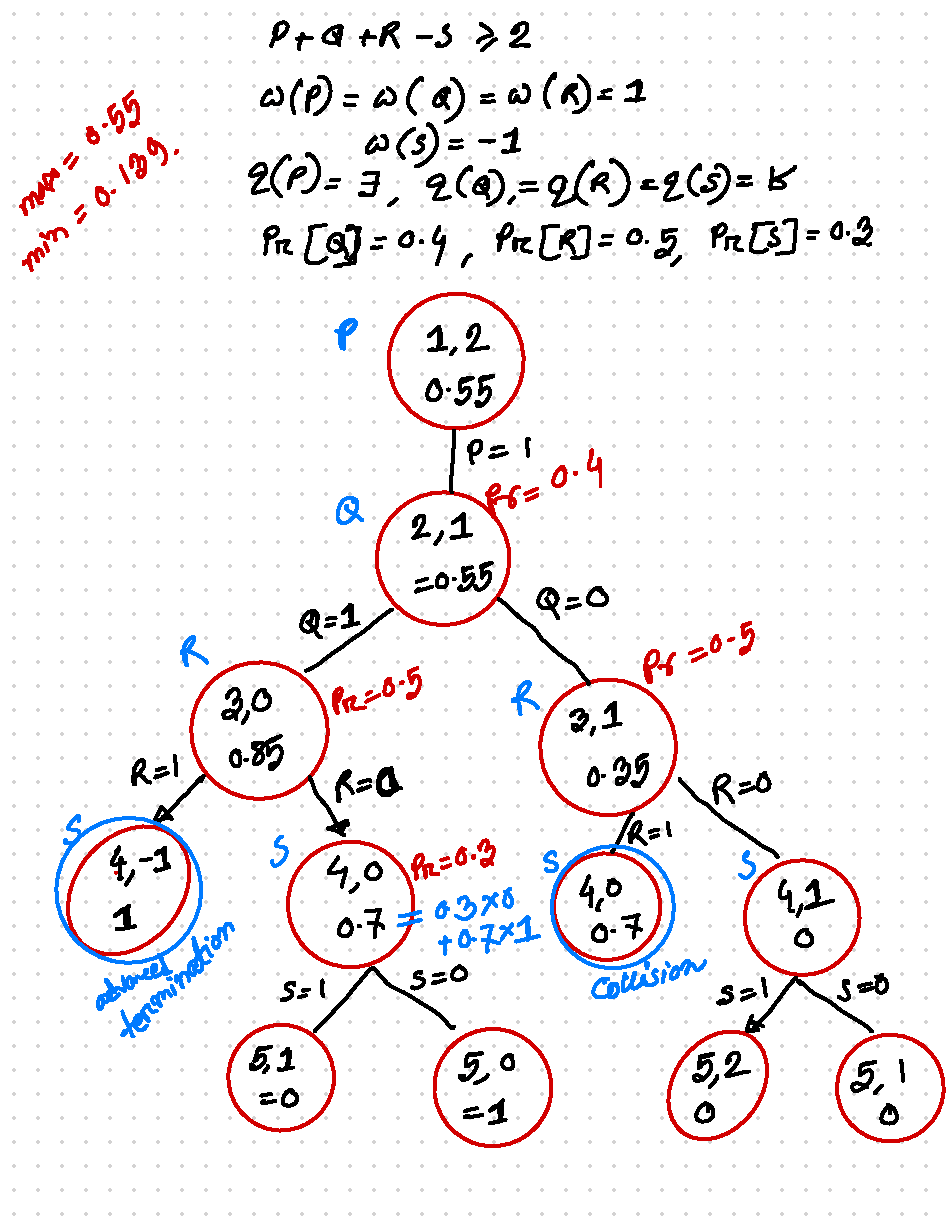
\includegraphics[scale=0.3]{figures/exploration_tree_DP}\label{fvgm_fig:example_dp}}
		\subfloat[Bayesian network]{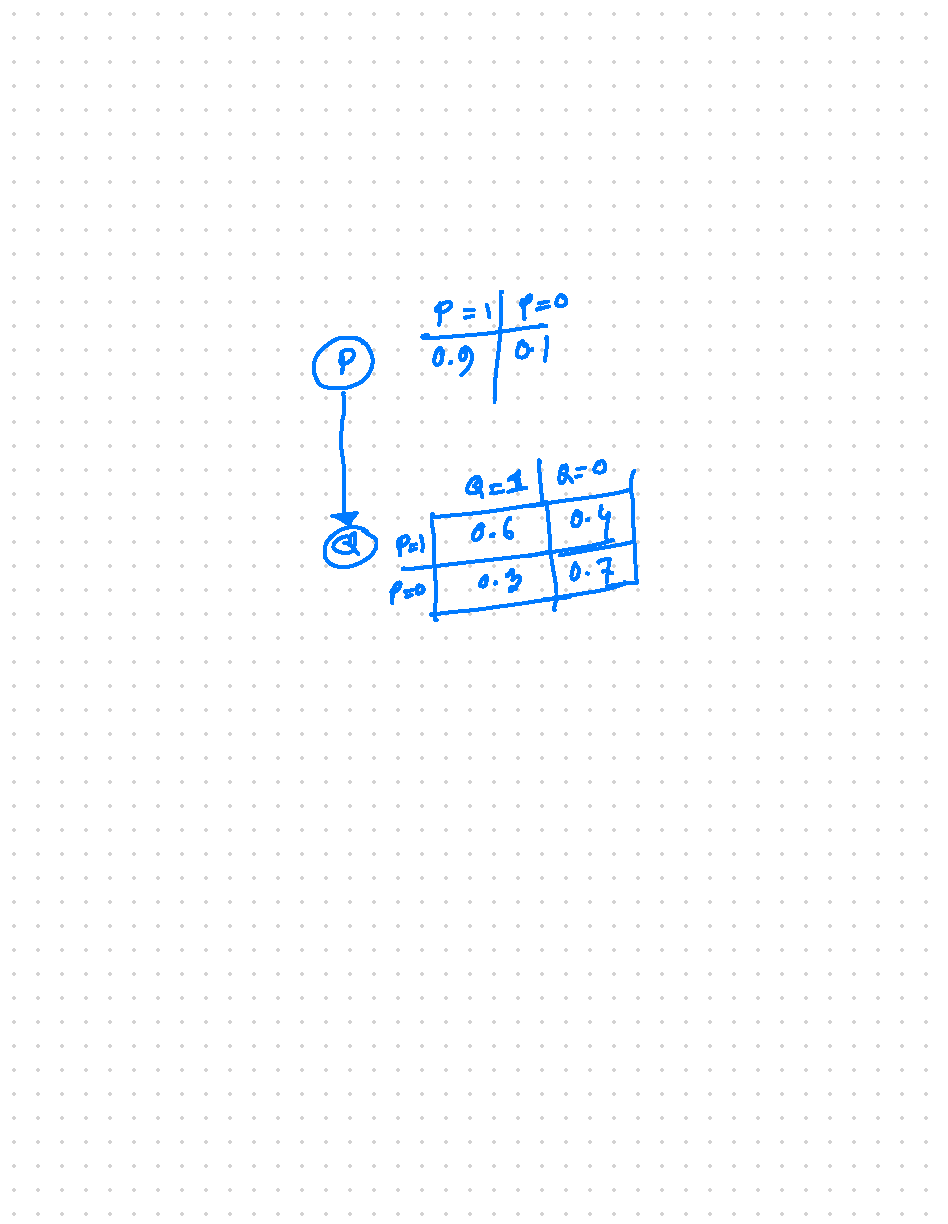
\includegraphics[scale=.4]{figures/example_BN}\label{fvgm_fig:example_BN}}
		\subfloat[Exploration tree of stochastic sub-set sum problem with Bayesian network]{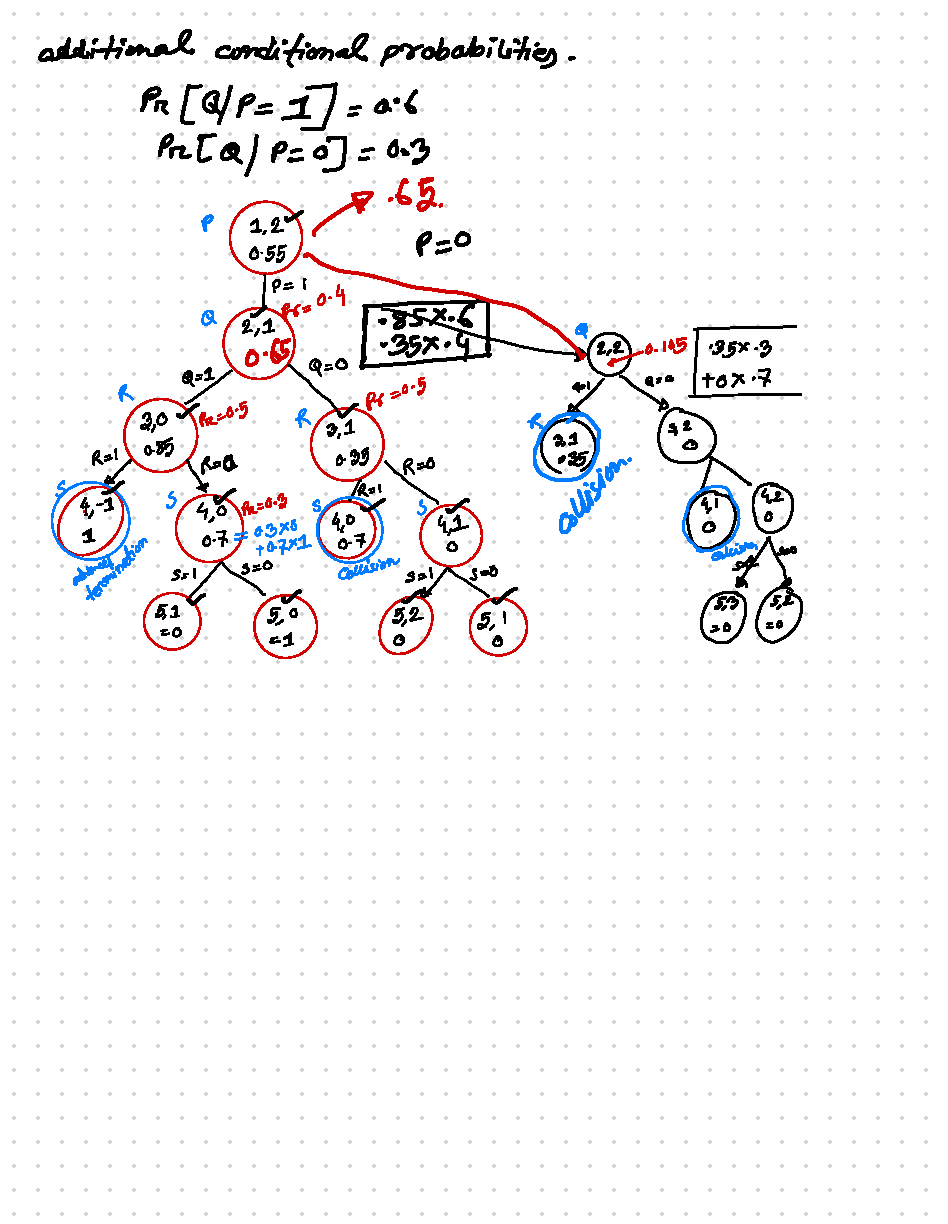
\includegraphics[scale=.4]{figures/exploration_tree_DP_BN}	\label{fvgm_fig:example_dp_BN}
		}
		
	\end{figure}
\end{comment}



				\section{Empirical Performance Analysis}
\label{fvgm_sec:experiments}
In this section, we empirically evaluate the performance of {\fvgm}. We first present the experimental setup and the objective of our experiments, followed by experimental results.
%\footnote{Due to page limit, we present additional experimental results, proof of lemmas, and miscellaneous details in Appendix.}

\begin{figure}[t!]
	\begin{center}		
		\subfloat{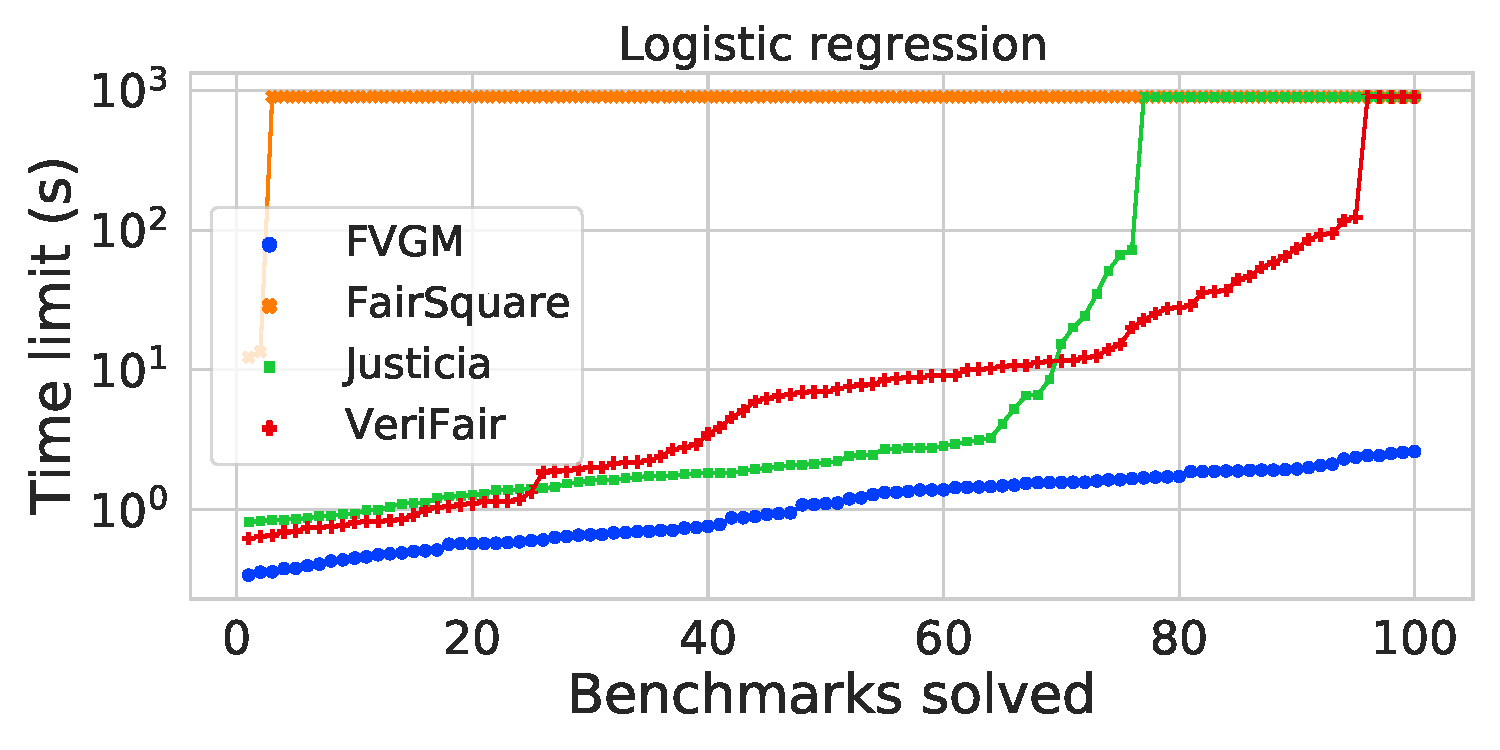
\includegraphics[scale=0.24]{figures/fairness/fvgm/cactus_all_verifiers_LR_time_}}\\
		\subfloat{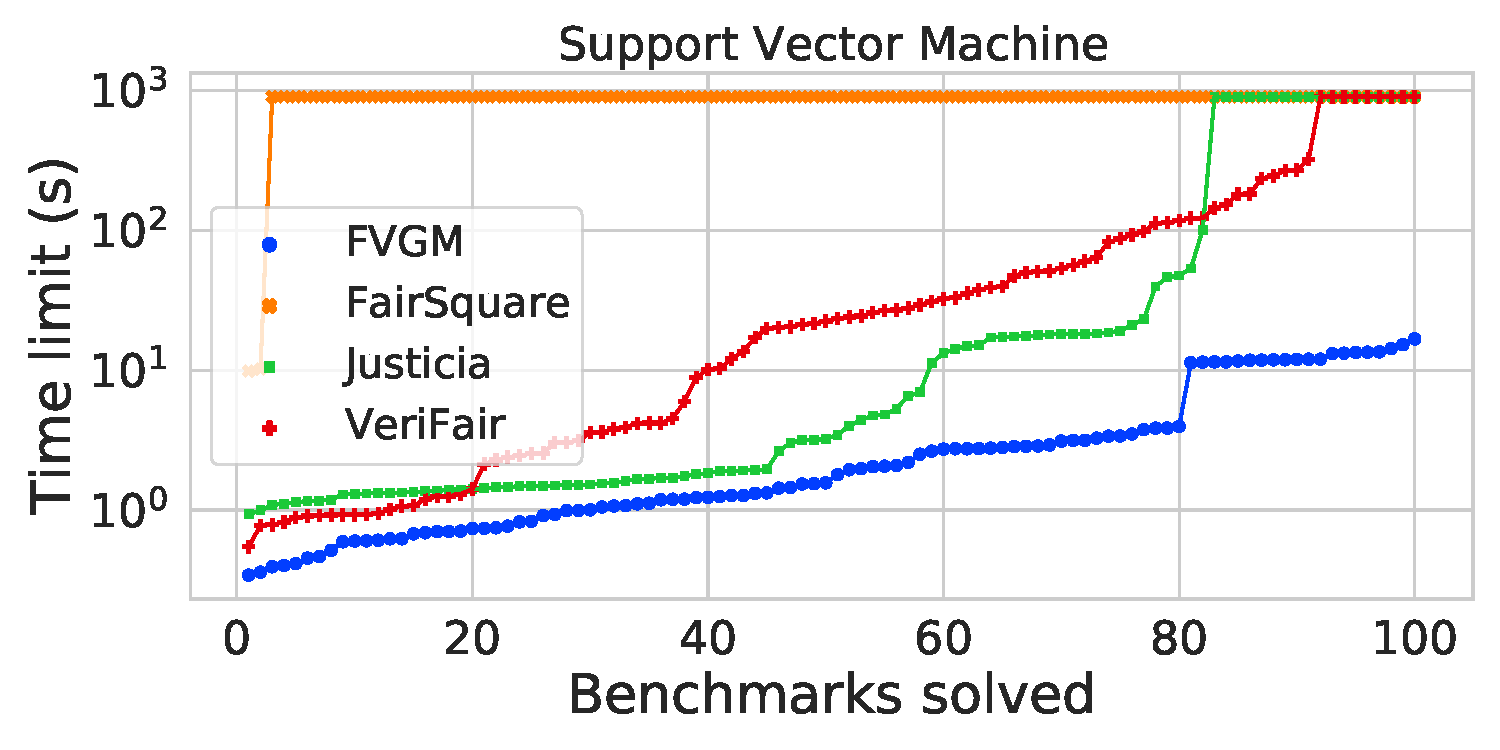
\includegraphics[scale=0.24]{figures/fairness/fvgm/cactus_all_verifiers_SVM_time_}}		
	\end{center}
	%	\vspace{-2ex}
	\caption{A cactus plot to present the scalability of different fairness verifiers. The number of solved benchmarks are on the $ X $-axis and the required time is on the $ Y $-axis; a point $ (x,y) $ implies that a verifier takes less than or equal to $ y $ seconds to compute fairness metrics of $ x $ many benchmarks. We consider $ 100 $ benchmarks generated from $ 5 $ real-world datasets using $ 5 $-fold cross-validation. In each fold, we consider $\{25, 50, 75, 100\} $ percent of non-sensitive features.}\label{fvgm_fig:scalability_exp}
	%	\vspace{-2ex}
\end{figure}

\textbf{Experimental Setup.}
We  implement a  prototype of {\fvgm} in Python (version 3.8).  
We deploy the Scikit-learn library for learning linear classifiers such as Logistic Regression (LR) and Support Vector Machine (SVM) with linear kernels. We perform five-fold cross-validation on a dataset. While the classifier is trained on continuous features, we discretize them to Boolean features to be invoked by {\fvgm}. During discretization, we apply a gird-search to estimate the best bin-size within a maximum bin of $ 10 $. To convert the coefficients of features into integers, we employ another grid-search to choose the best multiplier within $ \{1,2, \dots, 100\} $. For learning a Bayesian network on the converted Boolean data, we deploy the PGMPY library~\cite{ankan2015pgmpy}. For network learning, we apply a Hill-climbing search algorithm that learns a DAG structure by optimizing K2 score~\cite{koller2009probabilistic}. For estimating parameters of the network, we use Maximum Likelihood Estimation (MLE) algorithm. 

We compare {\fvgm} with three existing fairness verifiers: Justicia~\cite{ghosh2020justicia}, FairSquare~\cite{albarghouthi2017fairsquare}, and VeriFair~\cite{bastani2019probabilistic}. 
%Additionally, we have verified two fairness algorithms: reweighing algorithm (RW)~\cite{kamiran2012data} and the optimized pre-processing algorithm (OP)~\cite{calmon2017optimized}, and a fairness poisoning-attack algorithm~\cite{solans2020poisoning}. 


\subsection{Scalability Analysis}
\textbf{Benchmarks.} We perform the scalability analysis on five real-world datasets studied in fair ML literature: UCI Adult, German-credit~\cite{DK2017}, COMPAS~\cite{angwin2016machine}, Ricci~\cite{mcginley2010ricci}, and Titanic (\url{https://www.kaggle.com/c/titanic}). We consider $ 100 $ benchmarks generated from 5 real-world datasets and report the computation times (for DI and SP) of different verifiers.

\textbf{Results.} In Figure~\ref{fvgm_fig:scalability_exp}, we present the scalability results of different verifiers. First, we observe that FairSquare often times out ($ =900 $ seconds) and can solve $ \le 5 $ benchmarks. This indicates that SMT-based reduction for linear classifiers cannot scale. Similarly, SSAT-based verifier Justicia that performs pseudo-Boolean to CNF translation for linear classifiers, times out for around $  20 $ out of $ 100 $ benchmarks. Sampling-based framework, VeriFair, has comparatively better scalability than SMT/SSAT based frameworks and can solve more than $ 90 $ benchmarks. Finally, {\fvgm} achieves impressive scalability by solving all $ 100 $ benchmarks with $ 1 $ to $ 2 $ orders of magnitude runtime improvements than existing verifiers. Therefore,\textit{ {\stochastic}-based framework {\fvgm} proves to be highly scalable in verifying fairness properties of linear classifiers than the state-of-the-art.} 

\begin{figure}[t!]
	\begin{center}	
		\subfloat{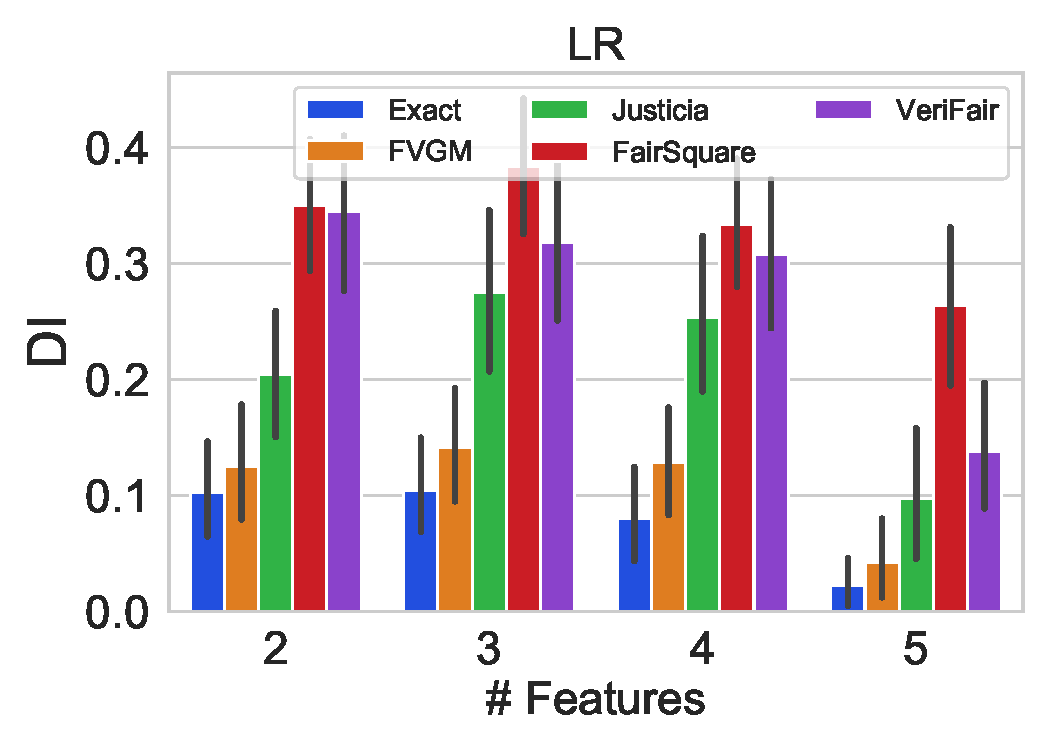
\includegraphics[scale=0.24]{figures/fairness/fvgm/sanity_DI_LR_01}}\\
		\subfloat{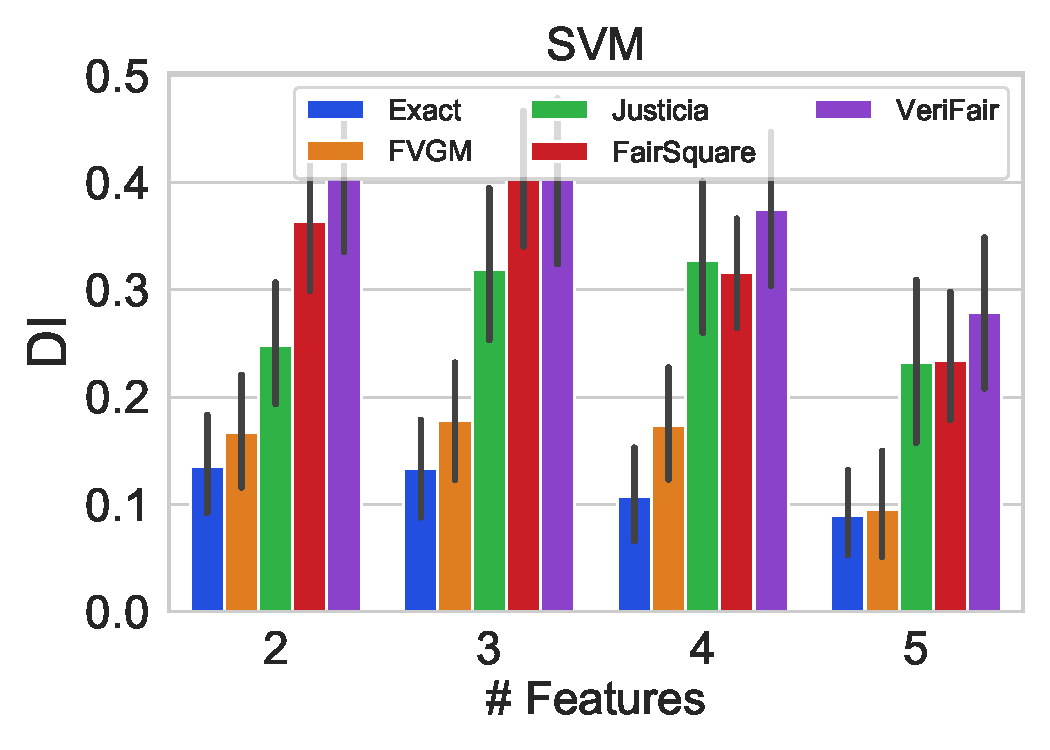
\includegraphics[scale=0.24]{figures/fairness/fvgm/sanity_DI_SVM_01}}		
		%		\subfloat[]{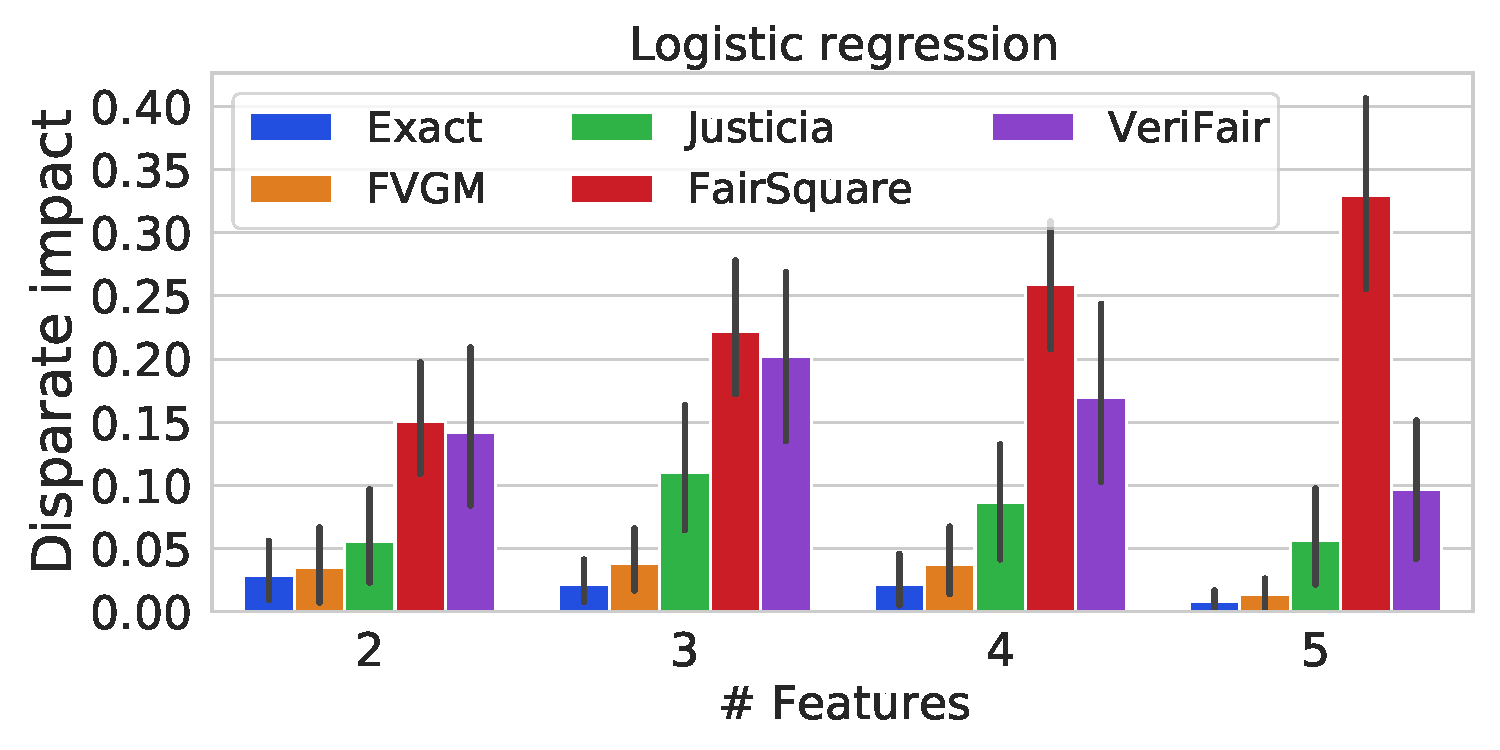
\includegraphics[scale=0.25]{figures/fairness/fvgm/sanity_DI_LR_005}}
		%		\subfloat[]{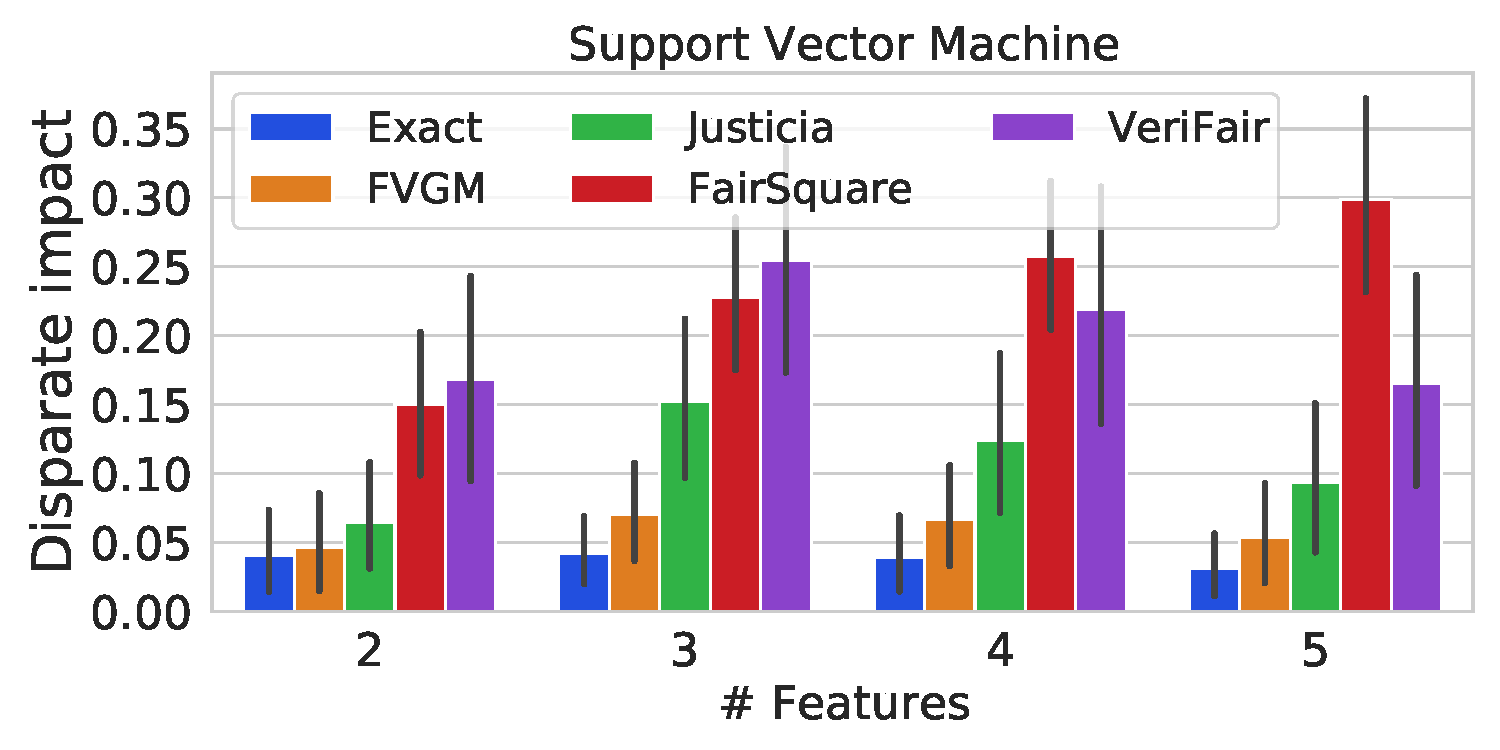
\includegraphics[scale=0.25]{figures/fairness/fvgm/sanity_DI_SVM_005}}
		%				
	\end{center}
	%	\vspace{-2ex}
	\caption{Comparing the average accuracy of different verifiers over 100 synthetic benchmarks while varying the number of features. {\fvgm} yields the closest estimation of the analytically calculated \textit{Exact} values of DI for LR and SVM classifiers.}\label{fvgm_fig:sanity_exp}
	%	\vspace{-2ex}
\end{figure}
\subsection{Accuracy Analysis}
\noindent\textbf{Benchmark Generation.} To perform accuracy analysis, we require the ground truth, which is not available for real-world instances. Therefore, we focus on generating synthetic benchmarks for analytically computing the ground truth of different fairness metrics, such as DI, from the known distribution of features. In each benchmark, we consider $ n \in \{2, 3, 4, 5\} $ features including one Boolean sensitive feature, say $ A $, generated from a Bernoulli distribution with mean $ 0.5 $.  We generate non-sensitive features $ X_i $ from Gaussian distributions such that   $ \Pr[X_i | A = 1] \sim \mathcal{N}(\mu_i, \sigma^2) $ and $ \Pr[X_i | A = 0] \sim \mathcal{N}(\mu_i', \sigma^2) $, where $ \mu_i, \mu_i' \in [0,1] $, $ \sigma = 0.1 $, and $ \mu_i, \mu_i' $ are chosen from a uniform distribution in $ [0,1] $. Finally, we create label $ Y = \mathds{1}[ \sum_{i=1}^{n-1} X_i \ge 0.5 \sum_{i=1}^{n-1} (\mu_i + \mu_i')] $ such that $ Y $ does not directly depend on the sensitive feature. For each $ n $, we generate $ 100 $ random benchmarks, learn LR and SVM classifiers on them, and compute DI\footnote{  
To analytically compute DI, let the coefficients of the classifier be $ w_i $ for $ X_i $ and $ w_A $ for $ A $, and bias be $ \tau $. Since all non-sensitive features are from Gaussian distributions, we compute the probability of the predicted class $ \Pr[\hat{Y} | A = 1]  \sim \mathcal{N}(\sum_{i=1}^{n-1}w_i\mu_i, \sigma_{\hat{Y}}^2) $ and $ \Pr[\hat{Y} | A = 0]  \sim \mathcal{N}(\sum_{i=1}^{n-1}w_i\mu_i', \sigma_{\hat{Y}}^2) $ with $ \sigma_{\hat{Y}}^2 =   (\sum_{i=1}^{n-1}w_i^2)\sigma^2 $. Hence, the PPV of the classifier  is $  1 - \mathsf{CDF}_{\hat{Y}| A =1}(\tau - w_A) $ for $ A = 1 $ and $  1 - \mathsf{CDF}_{\hat{Y}|A=0}(\tau) $ for $ A = 0 $, where $ \mathsf{CDF} $ is the cumulative distribution function. Finally, we compute DI by taking the ratio of the minimum and the maximum of the two PPVs.}
using different verifiers.



\textbf{Results.} 
%\begin{enumerate}[leftmargin=*]
%	\itemsep0em 
%	\item How \textit{accurate} is {\fvgm} w.r.t. existing verifiers?
%	\item How \textit{scalable} is {\fvgm} w.r.t. existing verifiers?
%	%\item Can {\fvgm} be applied to fairness problems such as \textit{verifying} different \textit{fairness metric}s for different \textit{fair ML algorithms} and \textit{fairness attacks}, and also \textit{detecting the sources of bias} due to different subset of features?
%\end{enumerate}
%To summarize our experimental results, {\fvgm} is more accurate and scalable than existing fairness verifiers in verifying linear classifiers on benchmark datasets. %{\fvgm} can verify diverse set of fairness metrics for multiple fairness-enhancing algorithms and depreciation attacks. {\fvgm} also computes fairness influence functions that can detect bias in the level of individual features. 
%\red{Due to limited space, we discuss additional experiments including verification of CNF-based classifiers with feature correlations and performance analysis of encoding Bayesian networks in Appendix.}
 We  assess the accuracy of the competing verifiers in estimating fairness metrics, specifically DI with LR and SVM classifiers. In Figure~\ref{fvgm_fig:sanity_exp}, {\fvgm} computes DI closest to the \textit{Exact} value for different number of features and both type of classifiers. In contrast, Justicia, FairSquare, and VeriFair measure DI far from the \textit{Exact} because of ignoring correlations among the features. For example, for SVM classifier with  $ n = 5 $ (right plot in Figure~\ref{fvgm_fig:sanity_exp}), \textit{Exact} DI is $ 0.089 $ (average over 100 random benchmarks). Here, {\fvgm} computes DI as $ 0.094 $, while all other verifiers compute DI as at least $ 0.233 $. Therefore, \textit{{\fvgm} is more accurate than existing verifiers as it explicitly considers correlations among features}. 








\begin{table}[!t]
		\centering
		
		
		\setlength{\tabcolsep}{0.45em}
		\begin{tabular}{lllrrrrrrrrrrrrr}
			
			\toprule
			Dataset & $ \sensitive $ & Algo. & $ \Delta $DI &  $ \Delta $PCF & $ \Delta $SP & $ \Delta $EO\\
			\midrule
			
			
			\multirow{4}{*}{\rotatebox[origin=c]{0}{Adult}}&\multirow{2}{*}{\rotatebox[origin=c]{0}{race}}&RW&$ \textbf{0.53} $&$ \textbf{-0.06} $&$ \textbf{-0.06} $&$ \textbf{-0.02} $\\
			&&OP&$ \textbf{0.57} $&$ \textbf{-0.07} $&$ \textbf{-0.07} $&$ \textbf{-0.02} $\\
			\cmidrule{2-7}
			&\multirow{2}{*}{\rotatebox[origin=c]{0}{sex}}&RW&$ \textbf{0.96} $&$ \textbf{-0.16} $&$ \textbf{-0.15} $&$ \textbf{-0.08} $\\
			&&OP&$ \textbf{0.43} $&$ \textbf{-0.08} $&$ \textbf{-0.08} $&$ 0.03 $\\
			
			
			\midrule
			\multirow{4}{*}{COMPAS}&\multirow{2}{*}{race}&RW&$ \textbf{0.13} $&$ \textbf{-0.07} $&$ \textbf{-0.07} $&$ \textbf{-0.06} $\\
			&&OP&$ \textbf{0.15} $&$ \textbf{-0.08} $&$ \textbf{-0.08} $&$ \textbf{-0.05} $\\
			\cmidrule{2-7}
			&\multirow{2}{*}{sex}&RW&$ \textbf{0.1} $&$ \textbf{-0.04} $&$ \textbf{-0.04} $&$ 0.04 $\\
			&&OP&$ \textbf{0.09} $&$ \textbf{-0.04} $&$ \textbf{-0.04} $&$ \textbf{-0.03} $\\
			
			\midrule
			\multirow{4}{*}{German}&\multirow{2}{*}{age}&RW&$ \textbf{0.52} $&$ \textbf{-0.53} $&$ \textbf{-0.52} $&$ \textbf{-0.47} $\\
			&&OP&$ \textbf{0.53} $&$ \textbf{-0.53} $&$ \textbf{-0.53} $&$ \textbf{-0.51} $\\
			\cmidrule{2-7}
			&\multirow{2}{*}{sex}&RW&$ -0.06 $&$ 0.06 $&$ 0.06 $&$ 0.02 $\\
			&&OP&$ -0.12 $&$ 0.12 $&$ 0.12 $&$ 0.07 $\\
			
			
			\bottomrule
		\end{tabular}
	
	\caption{Verification of fairness algorithms using {\fvgm}. $ \sensitive $ denotes sensitive features.  RW and OP refer to reweighing and optimized-preprocessing algorithms. Numbers in bold refer to fairness improvement.   }\label{fvgm_tab:fair_algo_verification}
		
		
	
\end{table}









%\begin{table}[!t]
%	\begin{minipage}{0.6\columnwidth}
%		\centering
%		\small
%		
%		\setlength{\tabcolsep}{.25em}
%		
%		\begin{tabular}{lllrrrrrrrrrrrrr}
%			
%			\toprule
%			$\mathbf{D}$ & $ \sensitive $ & Algo. & $ \Delta $DI &  $ \Delta $PCF & $ \Delta $SP & $ \Delta $EO\\
%			\midrule
%			
%			
%			\multirow{4}{*}{\rotatebox[origin=c]{90}{Adult}}&\multirow{2}{*}{\rotatebox[origin=c]{90}{race}}&RW&$ \textbf{0.53} $&$ \textbf{-0.06} $&$ \textbf{-0.06} $&$ \textbf{-0.02} $\\
%			&&OP&$ \textbf{0.57} $&$ \textbf{-0.07} $&$ \textbf{-0.07} $&$ \textbf{-0.02} $\\
%			\cmidrule{2-7}
%			&\multirow{2}{*}{\rotatebox[origin=c]{90}{sex}}&RW&$ \textbf{0.96} $&$ \textbf{-0.16} $&$ \textbf{-0.15} $&$ \textbf{-0.08} $\\
%			&&OP&$ \textbf{0.43} $&$ \textbf{-0.08} $&$ \textbf{-0.08} $&$ 0.03 $\\
%			
%			\bottomrule
%		\end{tabular}
%		
%		\caption{\footnotesize Verification of fairness algorithms using {\fvgm}. $ \mathbf{D} $ and $ \sensitive $ denote dataset and sensitive features.  RW and OP refer to reweighing and optimized-preprocessing algorithms. Numbers in bold refer to fairness improvement.   }\label{fvgm_tab:fair_algo_verification}
%		
%	\end{minipage}\hspace*{1em}
%	\begin{minipage}{0.4\columnwidth}
%		\centering
%		\subfloat{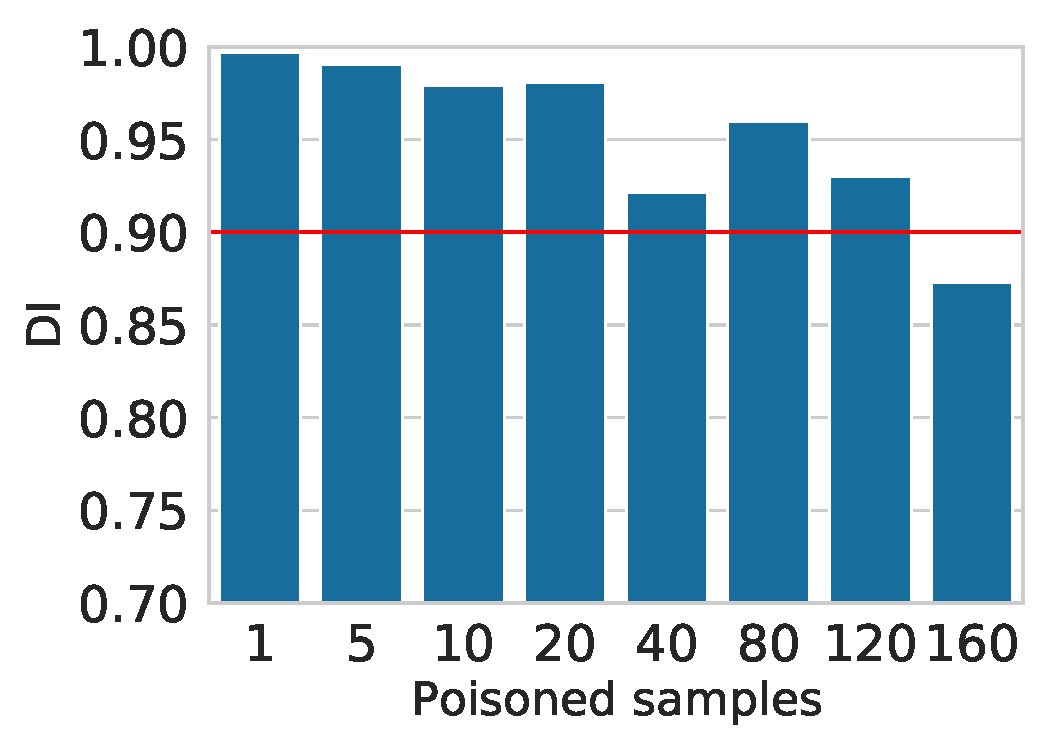
\includegraphics[scale=0.2]{figures/fairness/fvgm/disp_fairness_attack}}
%		\captionof{figure}{\footnotesize Verifying poisoning attack against fairness using {\fvgm}. The red line denotes the safety margin of the ML model against the attack.}\label{fvgm_fig:fairness_attacks}
%	\end{minipage}\hspace*{1em}
%%	\vspace{-2ex}
%	
%\end{table}


				\section{Applications of {\fvgm}}\label{fvgm_sec:applications}
In this section, we apply {\fvgm} for verifying fairness-enhancing algorithms and depreciation attacks. We also demonstrate that {\fvgm} facilitates the computation of fairness influence functions by enabling the shift of bias from the original value due to individual features. 


\iffalse
\begin{figure}[t!]
	%\vspace{-1em}
	
	\centering
	\subfloat{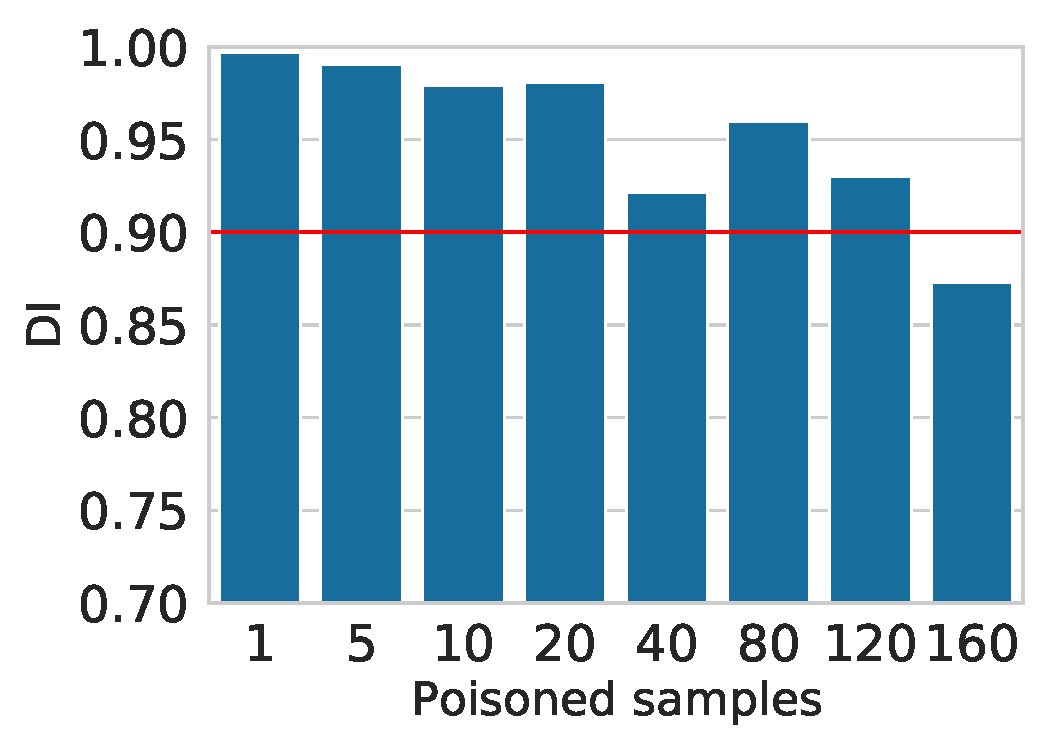
\includegraphics[scale=0.25]{figures/fairness/fvgm/disp_fairness_attack}}
	\subfloat{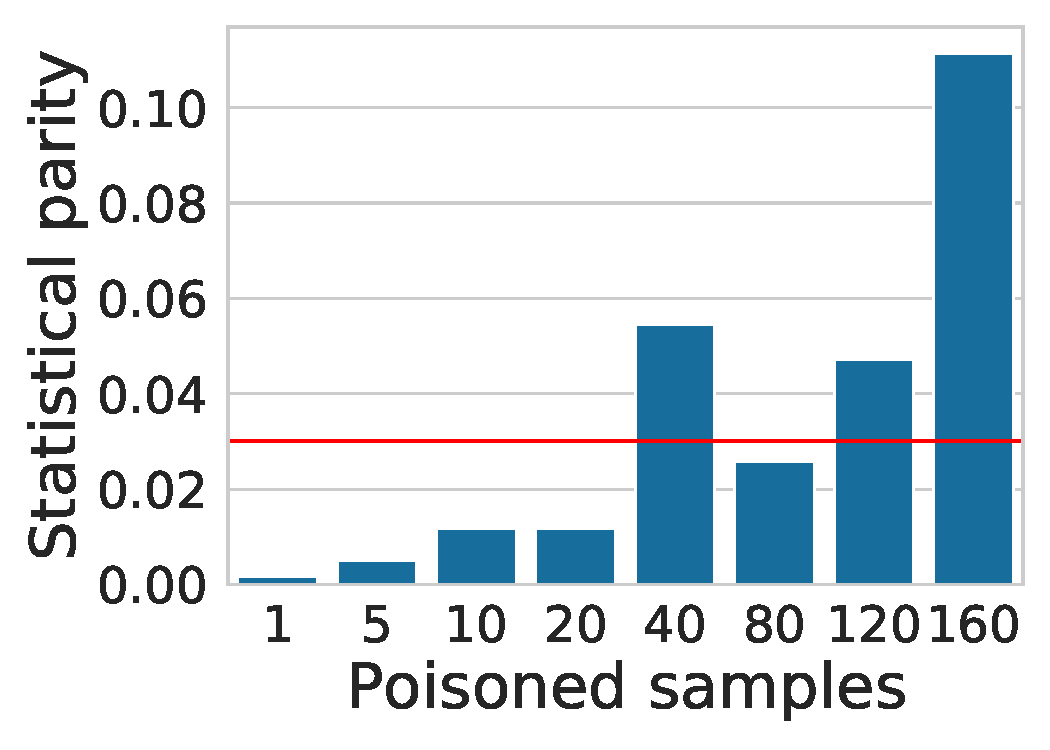
\includegraphics[scale=0.25]{figures/fairness/fvgm/stat_fairness_attack}}
	%\vspace{-0.5em}
	\caption{Verifying poisoning attack against fairness using {\fvgm}. The red line denotes the safety margin of the ML model against the attack.}\label{fvgm_fig:fairness_attacks}
\end{figure}
\fi


\paragraph{Verifying Fairness-enhancing Algorithms.} We deploy {\fvgm} in verifying the effectiveness of fairness-enhancing algorithms designed to ameliorate bias. For example, fairness 
pre-processing algorithms can be validated by applying {\fvgm} on the unprocessed and the processed data separately and comparing different fairness metrics. In Table~\ref{fvgm_tab:fair_algo_verification}, we report the effect of fairness algorithms w.r.t. four fairness metrics: disparate impact ($ \mathsf{DI} $), path-specific causal fairness ($ \mathsf{PCF} $), statistical parity ($ \mathsf{SP} $), and equalized odds ($ \mathsf{EO} $). Note that, fairness is improved if $ \mathsf{DI} $ increases and the rest of the metrics decrease. For instance, in most instances for Adult dataset, reweighing (RW)~\cite{kamiran2012data} and optimized pre-processing (OP)~\cite{calmon2017optimized} algorithms are successful in improving fairness. The exceptional case is the unfairness regarding the sensitive feature `sex', where OP algorithm fails in improving fairness metric $ \mathsf{EO} $. Thus, \textit{{\fvgm} verifies the enhancement and decrement in fairness by  fairness-enhancing algorithms. }



\begin{figure}
	\centering
	\subfloat{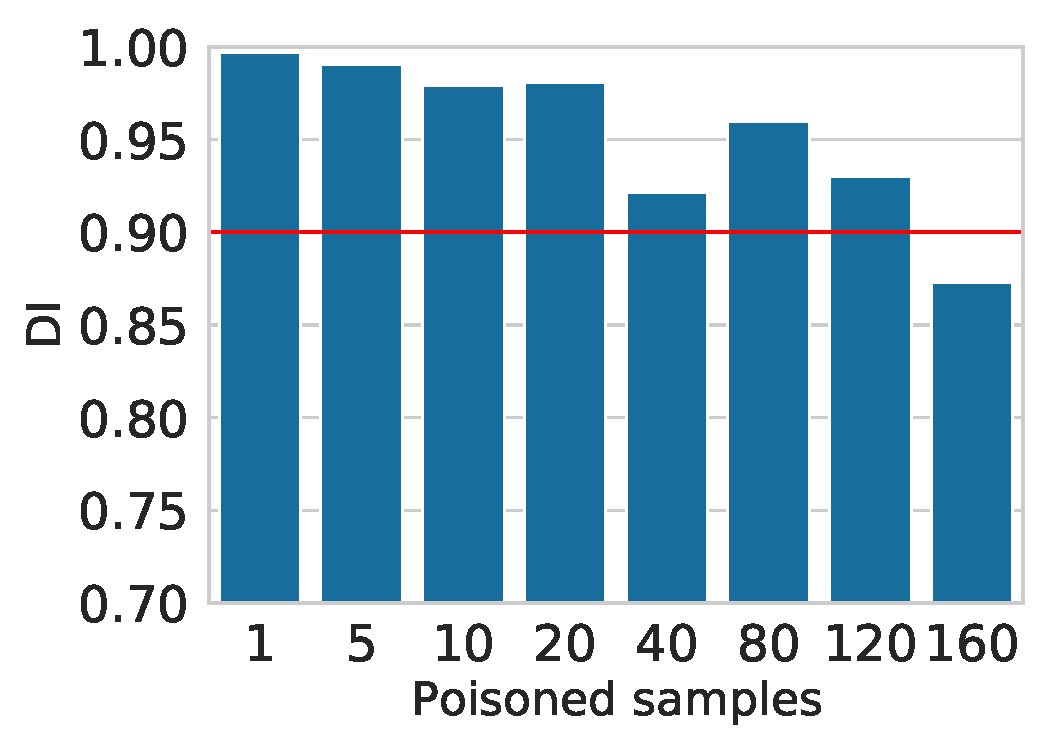
\includegraphics[scale=0.3]{figures/fairness/fvgm/disp_fairness_attack}}
	\subfloat{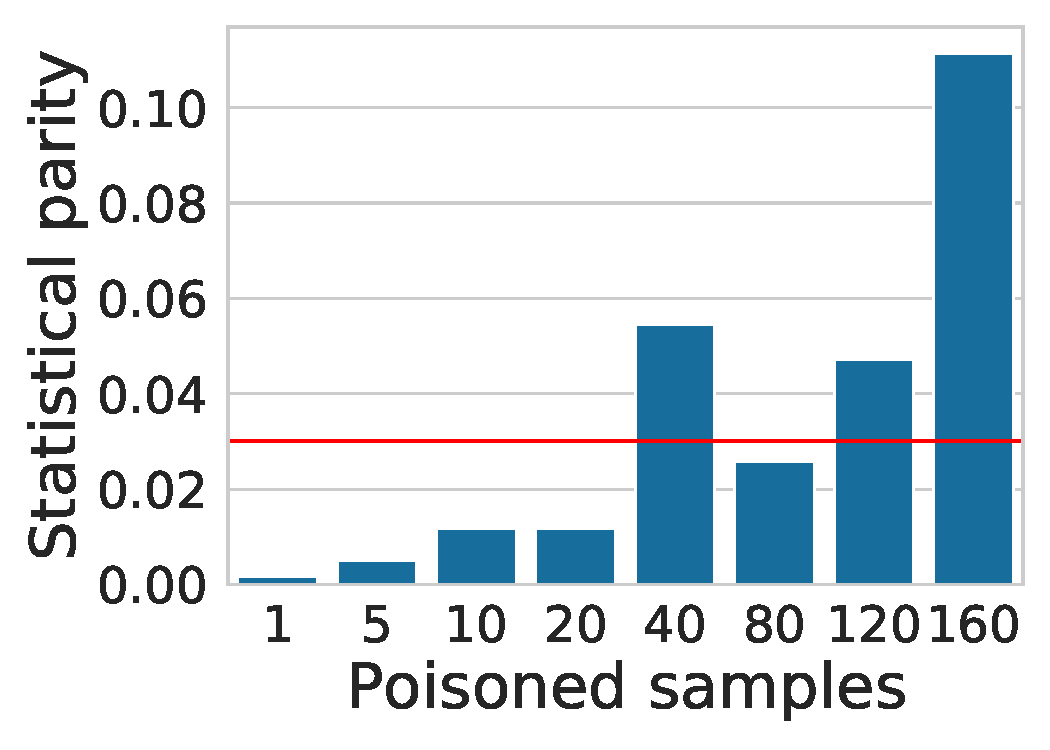
\includegraphics[scale=0.3]{figures/fairness/fvgm/stat_fairness_attack}}
	
	\caption[Verifying fairness attacks]{Verifying poisoning attack against fairness using {\fvgm}. The red line denotes the safety margin of the machine learning model against the attack.}\label{fvgm_fig:fairness_attacks}
\end{figure}


\paragraph{Verifying Fairness Attacks.}
We apply {\fvgm} in verifying a fairness poisoning-attack algorithm. This algorithm injects a small fraction of poisoned samples into the training data such that the classifier becomes relatively unfair~\cite{solans2020poisoning}. We apply this attack to add $\{1, 5, \dots, 160\}$ poisoned samples  and measure the corresponding disparate impact and statistical parity. In Figure~\ref{fvgm_fig:fairness_attacks},  {\fvgm} verifies that the disparate impact of the classifier decreases and statistical parity increases, i.e.\textit{ the classifier becomes more unfair},\textit{ as the number of poisoned samples increases}. Therefore, {\fvgm} shows the potential of being deployed in safety-critical applications to detect fairness attacks. For example, if we set $0.9$ as an acceptable threshold of disparate impact, {\fvgm} can raise an alarm once $160$ poisoned samples are added.


\iffalse
\begin{table}[!t]
	
	\centering
	\small
	\caption{Verification of fairness algorithms using {\fvgm}. Numbers in bold refer to fairness improvement. RW and OP refer to reweighing and optimized-preprocessing algorithms.  }\label{fvgm_tab:fair_algo_verification}
	\setlength{\tabcolsep}{.4em}
	
	\begin{tabular}{lllrrrrrrrrrrrrr}
		
		\toprule
		Dataset & Sensitive & Algo. & $ \Delta $ DI &  $ \Delta $ PCF & $ \Delta $ SP & $ \Delta $ EO\\
		\midrule
		
		
		\multirow{4}{*}{Adult}&\multirow{2}{*}{race}&RW&$ \textbf{0.53} $&$ \textbf{-0.06} $&$ \textbf{-0.06} $&$ \textbf{-0.02} $\\
		&&OP&$ \textbf{0.57} $&$ \textbf{-0.07} $&$ \textbf{-0.07} $&$ \textbf{-0.02} $\\
		\cmidrule{2-7}
		&\multirow{2}{*}{sex}&RW&$ \textbf{0.96} $&$ \textbf{-0.16} $&$ \textbf{-0.15} $&$ \textbf{-0.08} $\\
		&&OP&$ \textbf{0.43} $&$ \textbf{-0.08} $&$ \textbf{-0.08} $&$ 0.03 $\\
		
		\midrule
		\multirow{4}{*}{COMPAS}&\multirow{2}{*}{race}&RW&$ \textbf{0.13} $&$ \textbf{-0.07} $&$ \textbf{-0.07} $&$ \textbf{-0.06} $\\
		&&OP&$ \textbf{0.15} $&$ \textbf{-0.08} $&$ \textbf{-0.08} $&$ \textbf{-0.05} $\\
		\cmidrule{2-7}
		&\multirow{2}{*}{sex}&RW&$ \textbf{0.1} $&$ \textbf{-0.04} $&$ \textbf{-0.04} $&$ 0.04 $\\
		&&OP&$ \textbf{0.09} $&$ \textbf{-0.04} $&$ \textbf{-0.04} $&$ \textbf{-0.03} $\\
		
		\midrule
		\multirow{4}{*}{German}&\multirow{2}{*}{age}&RW&$ \textbf{0.52} $&$ \textbf{-0.53} $&$ \textbf{-0.52} $&$ \textbf{-0.47} $\\
		&&OP&$ \textbf{0.53} $&$ \textbf{-0.53} $&$ \textbf{-0.53} $&$ \textbf{-0.51} $\\
		\cmidrule{2-7}
		&\multirow{2}{*}{sex}&RW&$ -0.06 $&$ 0.06 $&$ 0.06 $&$ 0.02 $\\
		&&OP&$ -0.12 $&$ 0.12 $&$ 0.12 $&$ 0.07 $\\
		
		
		\bottomrule
	\end{tabular}
\end{table}
\fi




\paragraph{Fairness Influence Function (FIF): Tracing Sources of Unfairness.}
Another application of \fvgm{} as a fairness verifier is to quantify the effect of a subset of features on fairness. Thus, we define fairness influence function (FIF)  that computes the effect of a subset of non-sensitive features $\mathbf{S} \subseteq \nonsensitive$ on the probability of positive prediction of a classifier given a specific sensitive group $ \sensitive = \mathbf{a}$,
$
	\mathsf{FIF}(\mathbf{S}) \triangleq \Pr[\hat{Y} = 1 | \sensitive = \mathbf{a}, \mathcal{D}] - \Pr[\hat{Y} = 1 | \sensitive = \mathbf{a},  \mathcal{D}_{-\mathbf{S}}].
$
FIF allows us to explain the sources of unfairness in the classifier. In practice, we compute FIF of $\mathbf{S}$ by replacing the probability distribution of $\mathbf{S}$ with a uniformly random distribution, referred to as  $ \mathcal{D}_{-\mathbf{S}} $, and reporting differences in the conditional probability of positive prediction of the classifier. 

In Figure~\ref{fvgm_fig:influence function}, we compute FIF for all features in COMPAS dataset, separately for two sensitive groups: Female (`sex' $ = 1 $) and Male. This dataset concerns the likelihood of a person of re-offending crimes within the next two years. We first observe that the base values of the probability of positive prediction are different for the two groups ($ 0.46 $ vs $ 0.61 $ for Female and Male), thereby showing Male as more probable to re-offend crimes than Female. Moreover, FIF of the feature `age' is comparatively higher in magnitude for Male than Female. 
This implies that while deciding recidivism the algorithm assumes that Female individuals across different ages re-offend crimes with almost the same probability and the probability of re-offending for Male individuals highly depends on age. Thus, applying {\fvgm} to compute FIF provides us insights about sources of bias and thus, indicators to improve fairness.

\begin{figure}[t!]	
	\centering
	\vspace{-2ex}
	\subfloat{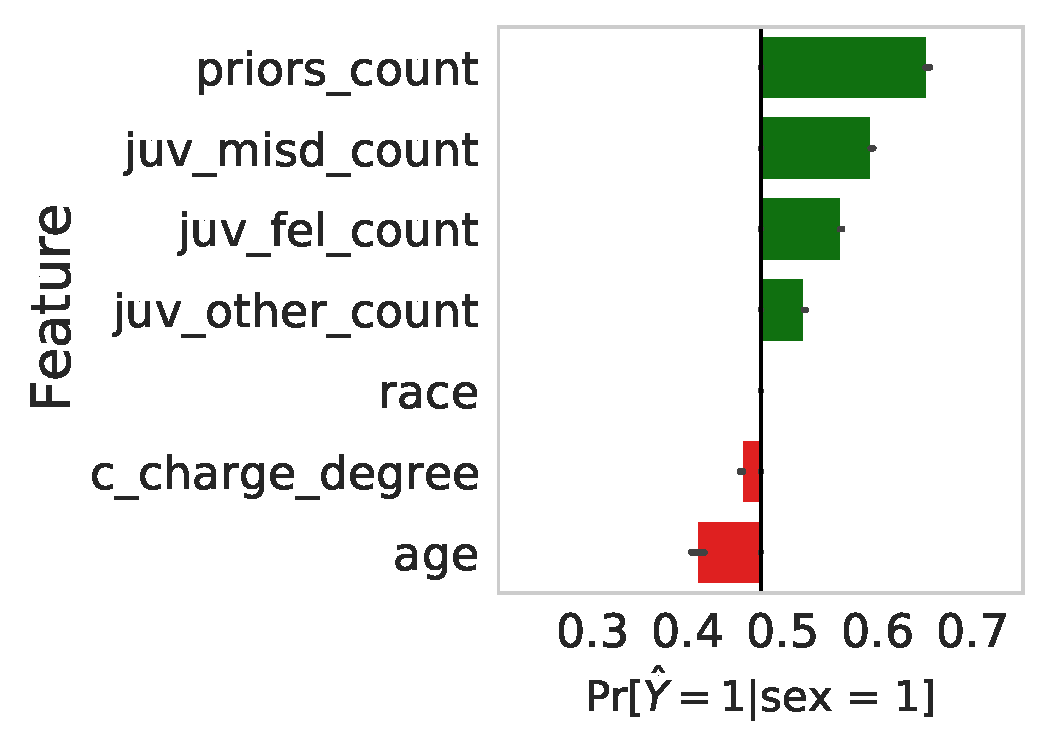
\includegraphics[scale=0.3]{figures/fairness/fvgm/dependency_exp_Learn-dependency_compas_lr_sex_1}}
	\subfloat{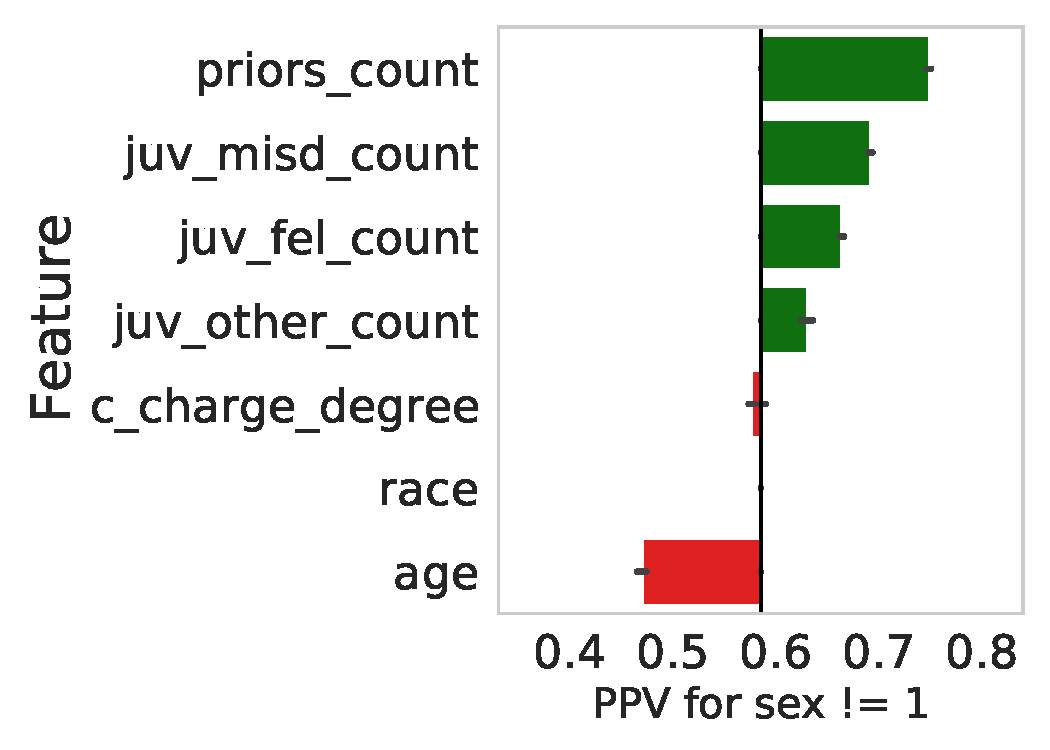
\includegraphics[scale=0.3]{figures/fairness/fvgm/dependency_exp_Learn-dependency_compas_lr_sex_0}}
	%\vspace{-0.5em}
%	\vspace{-2ex}
	\caption[FIF computation using {\fvgm}]{FIF computation for COMPAS dataset. For Female (left plot) and Male (right plot) individuals,  the influence of `age' decreases and the probability of positive prediction of the classifier increases  by different magnitudes.}\label{fvgm_fig:influence function}
%	\vspace{-2ex}
\end{figure}




				\section{Conclusion}
In this paper, we propose {\fvgm}, an efficient fairness verification framework for linear classifiers based on a novel stochastic subset-sum problem. {\fvgm} encodes a graphical model of feature-correlations, represented as a Bayesian Network, and computes multiple group and causal fairness metrics accurately. We experimentally demonstrate that {\fvgm} is not only more accurate and scalable than the existing verifiers but also applicable in practical fairness tasks, such as verifying fairness attacks and enhancing algorithms, and computing the fairness influence functions. 
As a future work, we aim to design fairness-enhancing algorithms certified by fairness verifiers, such as {\fvgm}. %We also investigate a principled approach to detect the sources of bias by computing fairness influence functions (FIF). 
Since {\fvgm} serves as an accurate and scalable fairness verifier for linear classifiers, it will be interesting to design such verifiers for other ML models.




				
				
			
		
			 
	
\bibliographystyle{siamurl}
\bibliography{ref}

\clearpage
\end{document}
